\documentclass{ctexart}%ctex自带中文包,不用再增加CJK

\usepackage{graphicx}
\usepackage{amsmath,amsthm}
\usepackage{amsfonts}
\usepackage{mathrsfs}
\usepackage{geometry}
\usepackage{xypic}
\usepackage{hyperref}
\usepackage{dynkin-diagrams}
\usepackage{tikz}

\usetikzlibrary{fit}
\newcommand\addvmargin[1]{
  \node[fit=(current bounding box),inner ysep=#1,inner xsep=0]{};
}
  
% ----------------------------------------------------------------
% AMS-LaTeX Paper ************************************************
% **** -----------------------------------------------------------
% ----------------------------------------------------------------
\vfuzz2pt % Don't report over-full v-boxes if over-edge is small
\hfuzz2pt % Don't report over-full h-boxes if over-edge is small
% THEOREMS -------------------------------------------------------

\newtheorem{theorem}{定理}
\newtheorem{lemma}{引理}
\newtheorem{proposition}{命题}
\newtheorem{corollary}{推论}
\theoremstyle{definition}
\newtheorem{definition}{定义}
\theoremstyle{remark}
\newtheorem{remark}{注}
%\newtheorem{proof}{证}
%\newtheorem{thm}{Theorem}[section]
%\newtheorem{cor}[thm]{Corollary}
%\newtheorem{lem}[thm]{Lemma}
%\newtheorem{prop}[thm]{Proposition}
%\theoremstyle{definition}
%\newtheorem{defn}[thm]{Definition}
%\theoremstyle{remark}
%\newtheorem{rem}[thm]{Remark}
%\numberwithin{equation}{section}
% MATH -----------------------------------------------------------
%\newcommand{\norm}[1]{\left\Vert#1\right\Vert}
%\newcommand{\abs}[1]{\left\vert#1\right\vert}
%\newcommand{\set}[1]{\left\{#1\right\}}
%\newcommand{\Real}{\mathbb R}
%\newcommand{\eps}{\varepsilon}
%\newcommand{\To}{\longrightarrow}
%\newcommand{\BX}{\mathbf{B}(X)}
%\newcommand{\A}{\mathcal{A}}
% ----------------------------------------------------------------


\DeclareMathOperator{\ad}{ad}
\DeclareMathOperator{\Tr}{Tr}
\DeclareMathOperator{\Rad}{Rad}
\DeclareMathOperator{\End}{End}
\DeclareMathOperator{\Der}{Der}
\DeclareMathOperator{\Hom}{Hom}
\DeclareMathOperator{\Ker}{Ker}
\DeclareMathOperator{\Int}{Int}
\DeclareMathOperator{\Res}{Res}
\DeclareMathOperator{\diag}{diag}

\newcommand{\Mod}[1]{\mathrm{mod}\ #1}


\tikzset{>=latex}


\begin{document}

\title{Lie Groups, Lie Algebras and Representations}

\author{Chunxiao Liu}

\maketitle



\section{一至六节}

$L$是域$\mathsf{F}$上的向量空间. 若在这之上又定义操作$L\times L\rightarrow L\colon (x,y)\mapsto [xy]$, 称为$x$和$y$的\textbf{交换子}, 满足以下性质: (1) 交换子对$x$和$y$为双线性; (2)对任意$x\in L$, $[xx]=0$; (3)对任意$x,y,z\in L$, Yacobi 恒等式成立$[x[yz]]+[y[zx]]+[z[xy]]=0$, 则称$L$为$\mathsf{F}$上的\textbf{李代数}. 注意, 李代数的定义并没有对$x$与$y$的``乘积''\;$xy$给出定义, 而只有``乘积括号''\;$[xy]$的定义. $L$的一个子集$K$称为$L$的子代数若$\forall x,y\in K$, $[xy]\in K$. 显然$K$的子代数自身也是一个李代数(乘法定义由$L$继承得到).

对于$\mathsf{F}$上的向量空间$V$, 定义$\End V$为$V$上的线性变换. 注意$\End V$有加法和乘法两种运算(加法继承向量空间加法; 乘法为复合), 故是一个环,故对$x,y\in \End V$可定义符号$[x,y]=xy-yx$, 使得$\End V$也成为一个李代数, 记为$\mathfrak{gl}(V)$, 称为一般线性李代数; 任何$\mathfrak{gl}(V)$的子代数, 称为线性李代数. 注意, 对线性李代数的交换子都是定义为$[x,y]=xy-yx$: 本书严格区分记号$[xy]$和$[x,y]$: 前者是一种满足(1-3)的抽象操作$L\times L\rightarrow L$, 后者则是特别定义的$xy-yx$; 前者只定义了交换子$[xy]$而没有定义乘法$xy$, 而后者具有事先定义好的乘法$xy$且$[x,y]$的定义基于乘法定义.

李代数$L$的一个\textbf{表示}是一个由(抽象)李代数$L$到线性李代数的同态$\phi\colon L\rightarrow \mathfrak{gl}(V)$, $V$是$\mathsf{F}$上的向量空间. 注意$L$本身也是一个向量空间, 故可谈$L$到$\mathfrak{gl}(L)$的同态. 这其中最重要的一个表示称作\textbf{伴随表示}, 记为$\ad \colon L\rightarrow \mathfrak{gl}(L)$, $x\mapsto \ad x$, 其中$\ad x$为$L$上的自同态, 满足$\ad x\colon L\rightarrow L$, $y\mapsto \ad x(y)\equiv[xy]$. 有时为了强调$\ad x$作用在$L$上, 我们用记号$\ad_L x$. 现在区分几个符号: $\ad$作为一个从李代数$L$到线性李代数$\mathfrak{gl}(L)$的同态, 是李代数的一个表示; $\ad L\subset \mathfrak{gl}(L)$是$L$在表示下的像, 是$L$上一些自同态的集合, 是$\mathfrak{gl}(L)$的一个子集, 从而是一个线性(子)李代数, 且其上的交换运算$[\ad x\,\ad y]$就定义为$[\ad x,\ad y]$(见上方分析). 一个重要的等式: 对于$x,y,z\in L$, 有
\begin{equation}\label{xy}
\begin{aligned}
{}[\ad x,\ad y](z) &= \ad  x \ad  y(z)-\ad  y \ad  x(z)
= \ad  x([yz])-\ad  y([xz])\\
&= [x[yz]]-[y[xz]]=[x[yz]]+[y[zx]]=-[z[xy]]=[[xy]z]=\ad  [xy] (z),
\end{aligned}
\end{equation}
其中用到了Jacobi恒等式. 从而$[\ad x,\ad y]=\ad  [xy]$. 伴随表示在李代数理论中有着举足轻重的地位, 因为它建立了抽象李代数$L$与线性李代数的联系而不借助任何其他额外资料. 注意$\Ker \ad = \{x\in L|\ad L(x)=[Lx]=0\}= Z(L)$, 即李代数$L$的\textbf{中心}. 


$L$是一个李代数, 其子空间$I$称为$L$的一个\textbf{理想}, 如果$x\in L$, $y\in I$导致$[xy]\in I$, 或简写为: $I$为$L$的一个理想如果$[LI]\subset I$. $L$的理想$I$天然是$L$的一个子(李)代数. 除了两个平凡理想$0$和$L^{(0)}:=L$, 还有两个特殊的$L$的理想是$L$的中心$Z(L)$, 和$L$的\textbf{导出李代数}$L^{(1)}:=[LL]$. 显然, $L$为阿贝尔的当且仅当导出子代数为零$[LL]=0$. 若$I$, $J$为李代数$L$的两个理想, 则$I+J:=\{x+y|x\in I, y\in J\}$也为$L$的一个理想($[I+J\,L]=[IL]+[JL]\subset I+J$). 类似地, $[IJ]=\{\sum_i [x_iy_i]|x_i\in I, y_i \in J\}$也为$L$的一个理想($[[xy]L]=-[[yL]x]-[[Lx]y]\subset[Jx]+[Iy]\subset [IJ]$). 在这个意义上$L$的导出李代数$[LL]$只是$[IJ]$的一个特例. 李代数称为\textbf{单的}(simple), 如果其除了$0$和它自身之外没有其他理想, 且同时满足$[LL]\neq0$; 显然$L$是单李代数要求$[LL]=L$且$Z(L)=0$. (后面我们将看到, 半单李代数也满足$[LL]=L$.) 我们进一步定义序列 $L^{(i)}=[L^{(i-1)}L^{(i-1)}]$, 并称$L$是\textbf{可解的}, 如果存在非负整数$n$使$L^{(n)}=0$. 显然阿贝尔李代数可解; 特别地$Z(L)$可解. 设$S$是$L$的一个极大可解理想(即$[LS]\subset S$, 存在$m$使$S^{(m)}=0$, 且没有比$S$大且含$S$的理想), 可证这样的极大可解理想是唯一的 (用下方命题\ref{3.1}证: 若$I$为$L$的任何其他可解理想, 则命题\ref{3.1}(c)表明$S+I$也为$L$的可解理想且含$S$, 故由$S$的定义必有$S+I=S$, 从而$I\subset S$, 唯一性得证), 称为$L$的\textbf{根理想}, 或简称根(Radical), 记为$\Rad  L$. 李代数$L$称为\textbf{半单的}(semisimple), 如果$\Rad L=0$. 显然单李代数是半单的(单李代数只有平凡理想, 且由于单李代数的交换子是它自身故不可解). 显然半单李代数$L$不存在阿贝尔理想; 特别地, 半单李代数$L$的中心$Z(L)=0$. 



设$K$为$L$的一个子代数. 子代数$K$的\textbf{正规化子}定义为$N_L(K)=\{x\in L|[xK]\subset K\}$. 对任意$x,y\in N_L(K)$, 由于$[[xy]z]+[[zx]y]+[[yz]x]=0$ $\forall z \in K$, 可见$[[xy]z]\in K$ 故$[xy]\in N_L(K)$, 从而$N_L(K)$是$L$的一个子代数(但不一定是$L$的理想). 由正规化子定义可见$N_L(K)$是具有理想$K$的$L$的最大的子代数.


定义李代数$L$的一个理想序列: $L^0=L$, $L^1=[LL](=L^{(1)})$,..., $L^i=[LL^{i-1}]$, 称为下降中心序列或下中心序列, $L$称为\textbf{幂零的}, 如果对某个$n$, $L^n=0$. 还可以定义元素在伴随表示下的幂零概念: $L$为一个李代数, 对$x\in L$, $x$是\textbf{$\ad$-幂零的}, 如果存在$n$使$\ad x$为$\mathfrak{gl}(L)$上的幂零自同态(即$(\ad x)^n=0$). 

显然, $\forall i$, $L^{(i)}\subset L^i$, 从而幂零李代数为可解李代数.

\begin{proposition}\label{3.1}$L$是一个李代数. (a)若$L$可解, 则$L$所有的子代数及$L$在任何同态下的像都是幂零的; (b)若$I$是$L$的一个可解理想且使$L/I$可解, 则$L$自身可解; (c)若$I$, $J$都为$L$的可解理想, 则$I+J$也是$L$的可解理想.
\end{proposition}
\begin{proof}
(a): 由定义及对$i$归纳易得, 若$K$是$L$的一个子代数则$K^{(i)}\subset L^{(i)}$, 若$\phi\colon L\rightarrow M$为满射, 则$\phi(L^{(i)})= M^{(i)}$. (b)若$(L/I)^{(n)}=0$, 由(a)对$\pi\colon L\rightarrow L/I$看出$\pi(L^{(n)})=0$, 或$L^{(n)}\subset I=\Ker \pi$现在$I^{(m)}=0$, 则由$(L^{(i)})^{(j)}= L^{(i+j)}$可得 $L^{(n+m)}=0$. (c)由代数同态定理可证$(I+J)/J$和$I/(I\cap J)$同构, 从而$(I+J)/J$可解; 再由(b)可证.
\end{proof}

\begin{proposition}\label{3.2}$L$是一个李代数. (a)若$L$幂零, 则$L$所有的子代数及$L$在任何同态下的像都是幂零的; (b)若$L/Z(L)$幂零, 则$L$也为幂零; (c)若$L$为幂零且非零, 则$Z(L)\neq0$.
\end{proposition}
\begin{proof}
(a): 由定义及对$i$归纳易得, 若$K$是$L$的一个子代数则$K^i\subset L^i$, 若$\phi\colon L\rightarrow M$为满射, 则$\phi(L^i)= M^i$. (b)取任意$x_1,...,x_n,y\in L$, 则由$(L/Z(L))^n=0$, 有$\ad (x_1+Z(L))\cdots \ad (x_n+Z(L))(y+Z(L)) = Z(L)$, 从而 $\ad x_1\cdots \ad x_n(y) \subset Z(L)$, 即 $L^n \subset Z(L)$, 从而$L^{n+1}=[L\,L^n]\subset [L\,Z(L)]=0$. (c)若$L^n=0$, 且$L^{n-1}\neq 0$, 即$[L\, L^{n-1}]=0$, 则$0\neq L^{n-1}\subset Z(L)$.
\end{proof}

\begin{theorem}\label{3.3}$L$为$\mathfrak{gl}(V)$的子代数, $V$有限维. 若$L$的元素均为$V$上的幂零自同态, $V\neq 0$, 则存在$v\in V$, 使$L.v=0$.
\end{theorem}
\begin{proof}
注意现在讨论的是$\mathfrak{gl}(V)$的子代数, 故交换子定义为$[x,y]=xy-yx$. 对$\dim L$归纳: $\dim L = 1$时, $L$由某一个$V$的幂零自同态生成, 这个幂零自同态至少有一个$V$中的特征向量, 且对应特征值0, 故$\dim L = 1$成立. 对任意$\dim L$: 设$K\neq L$为$L$的任何一个子代数, $L$为幂零, 故由上方论断, $\ad_LK$(作为作用在$L$上的诱导表示这个李代数)是幂零的, 同时也可定义$\ad_{L/K}K$. 由于$\dim K <\dim L$, 据归纳假设, 存在$L/K$的元素$x+K\neq K$, 使其在$\ad_{L/K}K$作用下的像(在$\mathfrak{gl}(L/K)$中)为零, 也即对任何$y\in K$ 有 $\ad y (x+K) \subset K$, 或$[xy]\in K$, 即存在$x$使$[xK]\subset K$, 从而$K$属于$K$在$L$中的正规化子$N_L(K)$. 现选$K$为$L$的一个极大真子代数, 则由于$N_L(L)$是$L$的一个极大子代数(见上), 故只能$N_L(K)=L$, 从而$K$为$L$的一个理想. 若$\dim L/K >1$, 则$L/K$中的一个1维子代数在$\ad_{L/K}K$下的原像是一个真包含$K$的真子代数, 这是不可能的, 故必有$\dim L/K=1$, 从而必有$L=K+\mathsf{F}z$, $\forall z\in L\backslash K$. 对$K$用归纳假设, $W=\{v\in V|K.v=0\}$非零. 由于$K$为$L$的理想, $W$满足如下性质: 对$\forall x\in L$, $\forall y\in K$, $\forall w\in W$, 有$yx.w=xy.w-[x,y].w=0$ (后两者都为零: $y\in K$, 且因$x\in L= N_L(K)$故$[x,y]\in K$), 这说明$x.w\in W$, 即$L.W\subset W$. 特别地, $z.W\subset W$, 则$z$在$W$中有一个特征向量, 记为$v$, 对应特征值0, 从而$L.v=0$, 从而对$\dim L$得证.
\end{proof}
\begin{remark}
评注见Engel定理下方.
\end{remark}



\begin{theorem}(Engel) $L$的所有元素都为$\ad$-幂零的当且仅当$L$为幂零的.
\end{theorem}
\begin{proof}
充分性: 如果$L$是幂零的, 则$L$的所有元素都是$\ad$-幂零的: 若$L^n=0$, 则对$\forall x_1,...,x_n,y\in L$, $\ad x_1 \ad x_2...\ad x_n(y)=0$, 特别地, 对$\forall x\in L$, $(\ad x)^n=0$. 必要性: 注意到$\ad L$是$\mathfrak{gl}(L)$的子代数. 故若李代数$L$的所有元素都是$\ad$-幂零的, 那么就满足了定理\ref{3.3}的条件, 从而存在非零的$x \in L$, 使$\ad L(x)=0$, 即$[Lx]=0$, 从而$Z(L)\neq 0$. 因$L$的元素均是$\ad$-幂零的, $L/Z(L)$的元素也均是$\ad$-幂零的, 且$L/Z(L)$的维度严格小于$L$. 这样$L'=L/Z(L)$又符合了定理\ref{3.3}的条件且$\dim L'<\dim L$. 重复此步骤, 必有某个$L^{'\cdots'}=0$则其为幂零的. 再重复利用上方命题\ref{3.2}的(b), 则$L$是幂零的.
\end{proof}
\begin{remark}
Engel定理很大程度上是定理\ref{3.3}的一个自然延伸. 定理\ref{3.3}是线性(李)代数的一个重要结论, 它说明了线性空间上的幂零自同态的集合有公共的特征向量(且该特征向量对应特征值0). 注意, 幂零自同态的集合自然地构成一个李代数.
\end{remark}


\begin{lemma}
设$x\in \mathfrak{gl}(V)$为$V$上的幂零自同态, 则$x$为$\ad$-幂零的.
\end{lemma}
\begin{proof}
注意要证的是$x$为$\ad$-幂零的, 即$\ad x\in\mathfrak{gl}(\mathfrak{gl}(V))$ 作为$\mathfrak{gl}(V)$上的自同态是幂零的. 这个映射当然就写为$\ad x$, 即$\forall y\in \mathfrak{gl}(V)$有$\ad x(y) =[x,y]=xy-yx$, 这样, 可以把$\ad x$看做两个映射的差: $\ad x= \lambda_x-\rho_x$, 这里$\lambda_x(y)=xy$, $\rho_x(y)=yx$. 注意$\rho_x$, $\lambda_x$作为$\mathfrak{gl}(V)$上的自同态都是幂零的($\rho_x^n(y)=yx^n=0$, $\lambda_x^n(y)=x^ny=0$), 而两个幂零映射的和或差都为幂零的(显然$(\rho_x-\lambda_x)^{2n}(y)=0$), 故$x$为$\ad$-幂零的.
\end{proof}

\begin{lemma}\label{3.3l}
设$L$为幂零, $K$为$L$的一个理想. 若$K\neq 0 $, 则$K\cap Z(L)\neq 0$. (特别地, $Z(L)\neq 0$, 即命题\ref{3.2}(c)的内容.)
\end{lemma}
\begin{proof}
$L$在$K$上有伴随表示, 从而定理\ref{3.3}保证存在非零$x\in K$,使$\ad L(x)=0$, 即$[Lx]=0$, 从而$x\in K\cap Z(L)$.
\end{proof}

\begin{remark}
现在有必要梳理一下几个幂零的概念. 首先, 对于一个向量空间$V$, 其上的自同态$x\in \End(V)$有幂零的概念, 即存在某个$n$使$x^n$为$V$上的零自同态. 这个定义源于线性代数, 故并未在此再次定义. 特别地, 选$V$为李代数的伴随表示空间$V=\mathfrak{gl}(L)$, 则李代数的元素$x\in L$在$V=\mathfrak{gl}(L)$上可以定义三个幂零的概念: $\rho_x$幂零, $\lambda_x$幂零, 或$\ad x=\rho_x-\lambda_x$幂零; 最后一个也就是我们之前定义过的$\ad$-幂零的概念. 其次, 我们还定义了李代数$L$是幂零的这一概念, 即存在某个$n$使$L^n=0$, 这里记号$L^n=[LL^{n-1}]$源自下降中心序列. 一个自然的问题是为何不定义$L$中元素$x$为幂零的这一概念. 原因是$x$为幂零的这一条件太强了, 没法很好地利用; 而较弱的条件''$L$是幂零的''则是一个不错的条件, 因为它等价于$L$的所有元素都为$\ad$-幂零的 (即Engel定理). Engel定理叙述了一个$L$的性质与$L$的任意元素都具有的性质之间的等价性, 这是这个定理很有意思的地方. 注意, 到此为止$L$都可以为任意李代数, 而非限制在线性李代数$L\subset \mathfrak{gl}(V)$. 若限制在线性李代数$L\subset \mathfrak{gl}(V)$, 则可考虑$x$作为$V$上自同态的幂零性, 我们也就得到了上述引理, 引理说明了线性李代数的元素的(作为自同态的)幂零性可以推出其$\ad$-幂零性. 但注意, 反之不成立: 如$\mathfrak{gl}(n,\mathsf{F})$中的单位矩阵$1$, 显然有$\ad 1$为零映射($1$与任何$x\in \mathfrak{gl}(n,\mathsf{F})$都交换), 故为幂零映射, 但其作为$\mathsf{F}^n$上的线性变换显然不是幂零映射.
\end{remark}

\begin{theorem}$L$为$\mathfrak{gl}(V)$的一个可解子李代数, $V$是$\mathsf{F}$上的有限维线性空间, $\mathrm{char}\,F =0$. 若$V\neq 0$, 则$V$中存在向量$v$, 它是$L$中所有元素($V$上自同态)的公共特征向量.
\end{theorem}

\begin{corollary}(Lie) $L$为$\mathfrak{gl}(V)$的一个可解子代数, $\dim V=n<\infty$. 则$L$在某组$V$的基下的矩阵为上三角.
\end{corollary}

\begin{corollary}设$L$是任意可解李代数. 则存在$L$的一个理想的链$0=L_0\subset L_1\subset \cdots \subset L_n=L$, 使得$\dim L_i = i$.
\end{corollary}

\begin{corollary}\label{4.1C}
设$L$为任意可解李代数, $x\in [LL]$. 则$\ad_L x$是幂零的; 特别地, $[LL]$是幂零的.
\end{corollary}

现在回忆线性代数中的Jordan-Chevalley分解. 设$V$为一个代数闭域$\mathsf{F}$ (但$\mathrm{char}F$可为任意)上的有限维向量空间, 对任何一个$x\in \End V$, Jordan-Chevalley分解定理表明存在一组基, 在这组基下$x$的矩阵为Jordan标准型. 定义$x\in \End  V$称为\textbf{半单的}, 若其最小多项式(注意, 是最小多项式)在$\mathrm{F}$上的根两两不同(见线性代数中的证明). 换言之, $x$为半单的当且仅当$x$可对角化 (线性代数中称半单为对角化). 进一步地, 两个交换的半单自同态可同时对角化, 从而其和或差也是半单的. 且如果$x$是半单, 且将$V$的子空间$W$映到$W$, 则$x$在$W$上的限制也是半单的. 

\begin{lemma}
若$x,y\in \End V$均为半单(即可对角化), 且$x$与$y$交换, 则$x$, $y$可同时对角化, 从而其和, 差, 积也是半单的.
\end{lemma}
\begin{proof}
证明见线性代数.
\end{proof}

\begin{proposition}\label{4.2}
$V$为$\mathsf{F}$上有限维向量空间, $x\in \End V$.

(a)存在唯一的$x_s,x_n \in \End V$使得$x=x_s+x_n$, 其中$x_s$为半单, $x_n$为幂零, $x_s$和$x_n$交换.

(b)存在单一变元的多项式$p$和$q$, 其常数项均为零, 使$x_s=p(x)$, $x_n=q(x)$. 特别地, $x_s$和$x_n$与$y\in \mathfrak{gl}(V)$交换, 这里$y$是任何与$x$交换的$V$的自同态.

(c)若$A\subset B\subset V$为子空间, 且$x$将$B$映到$A$, 则$x_s$和$x_n$也将$B$映到$A$.
\end{proposition}
满足上面条件的唯一分解$x=x_s+x_n$称为$x$的(加法)\;\textbf{Jordan-Chevalley分解}, 或简称Jordan分解, $x_s,x_n$分解叫做$x$的\textbf{半单部分}和\textbf{幂零部分}. 注意利用$x_s$的可逆性及加法Jordan分解, 也可以写出$x$的乘法Jordan分解.
\begin{proof}
设$a_1,...,a_k$(对应重数为$m_1,...,m_k$)为$x$的两两不同的特征值, 从而特征多项式为$\prod(T-a_i)^{m_i}$, 这里$T$只是一个无定义的符号. 定义$V_i =  \Ker(x-a_i\cdot 1)^{m_i}$, 则$V$可写成所有子空间$V_i$的直和, 且$x$把每个$V_i$映到$V_i$. 在$V_i$上, $x$显然具有特征多项式$(T-a_i)^{m_i}$. 现使用多项式环$\mathsf{F}[T]$上的中国剩余定理, 知存在$p(T)$, 满足对任意的$i$, $p(T)\equiv a_i \,(\Mod (T-a_i)^{m_i})$, 且$p(T)\equiv 0\,(\Mod T)$. 注意最后一个条件$p(T)\equiv 0\,(\Mod T)$: 如果存在一个$a_i=0$则显然存在这样的$p$; 否则, 对所有$(T-a_i)^{m_i}$及$T$用中国剩余定理也存在这样的$p$. 从而令$q(T)=T-p(T)$. 现定义$x_s=p(x), x_n=q(x)$. 由于$x_s,x_n$都为$x$的多项式, 故两者互相交换, 且都与任何其他与$x$交换的$V$的自同态交换, 则(b)得证. 若$x$把某个$V$的子空间映到自身, $x_s,x_n$也如此, 特别地, $x_s, x_n$也都把$V_i$映到$V_i$. 由$p(T)\equiv a_i(\Mod (T-a_i)^{m_i})$可见$x_s-a_i\cdot 1$在$V_i$上是零映射, 从而$x_s$在$V_i$上是对角的, 且有唯一特征值$a_i$. 根据定义, $x_n=x-x_s$为幂零的(从矩阵形式看出). 由于$p(T),q(T)$都没有常数项, 故(c)显然成立. 现只需证(a)中的唯一性: 令$x=s+n$为另一个满足条件的分解, 则$x_s-s=x_n-n$, 由(b), $x_s,s,x_n,n$均两两交换. 由于交换的两个半单(幂零)的$V$的自同态的和或差仍为半单的(幂零的), 故等式两边既幂零又半单, 但只有零映射满足. 从而唯一性得证.
\end{proof}

\begin{lemma}\label{4.2.A}设$x\in \End V$ ($V$有限维), $x=x_s+x_n$为$x$的Jordan分解. 则$\ad x=\ad x_s+\ad x_n$为$\ad x$的Jordan分解.
\end{lemma}
\begin{proof}
由于$x_s,x_n$分别为半单和幂零, 则$\ad x_s$和$\ad x_n$作为$\End V$上的自同态也为半单和幂零(半单: 可视为命题\ref{3.1}(a)作用于单生成元李代数$\langle x_s\rangle$的特殊情形; 幂零, 可用引理\ref{3.2}). 且$\ad x_s$, $\ad  x_n$交换(因$[\ad x_s,\ad x_n] = \ad [x_s,x_n]=0$), 故满足命题\ref{4.2}(a)的结论, 从而$\ad x=\ad x_s+\ad x_n$就是$\ad x$的Jordan分解.
\end{proof}

\begin{lemma}\label{4.3}
$A\subset B$为$\mathfrak{gl}(V)$的两个子空间, $V$有限维.定义$M=\{x\in \mathfrak{gl}(V)|[x,B]\subset A\}$. 设$x\in M$ 满足$\Tr(xy)=0$ $\forall y\in M$, 则 $x$为幂零的.
\end{lemma}
\begin{proof}
设$x=s+n$为$x$的Jordan分解. 选定$V$的一组基$v_1,...,v_m$, 使得在这组基下$s$的矩阵为$\diag(a_1,...,a_m)$ (这里特征值$a_1,...,a_m$中可能有相同的). 定义$E$为素域(prime field)$\mathbf{Q}$上由$a_1,...,a_m$张成的向量空间, 其为$\mathsf{F}$的一个子向量空间. 现要证的是, 对于满足引理条件的那样的$x$, 其半单部分$s=0$, 即证$E=0$. 由于$E$在$\mathbf{Q}$上维数有限维, 故只需证其对偶空间$E^*$为零, 即任何线性函数$f\colon E\rightarrow \mathbf{Q}$必为零. 给定任何一个映射$f\colon E\rightarrow \mathbf{Q}$, 则可找到$y\in\mathfrak{gl}(V)$, 其在基$v_1,...,v_m$上的矩阵为$\diag(f(a_1),...,f(a_m))$. 现设$\mathfrak{gl}(V)$的一组基是$\{e_{ij}\}$, 其中$e_{ij}=\delta_{ij}$是只把$v_j$映到$v_i$, 其他均为零的映射, 则$\ad s(e_{ij})=[s, e_{ij}]=se_{ij}-e_{ij}s = (a_i-a_j)e_{ij}$, 且$\ad y(e_{ij})= (f(a_i)-f(a_j)) e_{ij}$. 现令$r(T)\in \mathsf{F}[T]$为常数项为零的多项式且满足$r(a_i-a_j) = f(a_i)-f(a_j)$对任意$(i,j)$成立; $r$的存在性由Lagrange插值定理可证. 则$\ad y(e_{ij}) = r(a_i-a_j)e_{ij}= r(\ad s)(e_{ij})$, 从而$\ad y=r(\ad s)$. 由于$\ad s$是$\ad x$的半单部分(引理\ref{4.2.A}), 故由上方命题\ref{4.2}的中间结论, $\ad s$可以写为$\ad x$的多项式且不含常数项. 从而$\ad y$也是$\ad x$的一个多项式且不含常数项. 由假设, $\ad x$将$B$映入$A$, 故$\ad y$也将$B$映入$A$, 从而$y\in M$. 再利用假设$\Tr(xy)=0$, 有$\sum a_i f(a_i)=0$, 其左边是$E$中元素的$\mathbf{Q}$-线性组合, 故再用$f$作用一次, 得到$\sum f^2(a_i)=0$, 但$f(a_i)$是有理数, 故所有项都为零, 从而必有$f=0$ (因$a_i$张成$E$).
\end{proof}
\begin{remark}
这个证明看上去有些不直观. 其中的关键是对$\forall y\in M$这个条件的利用: 既然是最后证明$x$的性质, 那么就选$M$中的一些和$x$有关系的$y$, 这样题设条件$\Tr(xy)=0$就变成$x$的某个性质可以进行利用. 具体来说, 对任何$x=s+n$, 这里直接把$s$看成对角矩阵, 那就选$y$为$f(s)$, 这里$f$是任何一个$\mathsf{F}\rightarrow \mathsf{F}'$的函数, 其中$\mathsf{F}'$是某个数域. 接下来首先要证的就是$y$的确属于$M$, 思路如下: 发现可证$\ad y$是$\ad s$的不含常数项的多项式; 而$\ad s$(作为$\ad x$的半单部分)可写成$\ad x$的不含常数项的多项式(命题\ref{4.2}的中间结论), 从而$\ad y$可写成$\ad x$的不含常数项的多项式; 而$x\in M$意味着$\ad x (B)\subset A$, 故$\ad y(B)\subset A$, 即也有$y\in M$. 这之后, 就可以轻易地利用$\Tr(xy)=0$这个条件来证明$f=0$; 最后只需由$f=0$证$s=0$: 由于目前$f\colon \mathsf{F}\rightarrow \mathsf{F}'$是任意函数, 故只需要对$f$及$\mathsf{F}'$加以限制, 就可证; 具体的方法就是讲$\mathsf{F}'$限制为一个素域(即$\mathbf{Q}$), 且令$f$不是$\mathsf{F}$上的函数, 而是$\mathsf{F}$的一个子线性空间$E$上的函数, $E$是由$a_1,...,a_m$张成的$\mathbf{Q}$上的线性空间. 
\end{remark}
\begin{theorem}(Cartan) $L$为 $\mathfrak{gl}(V)$的一个子代数, $V$有限维. 若$\Tr(xy)=0$ $\forall x\in[LL]$及$y\in L$, 则$L$可解.
\end{theorem}
\begin{proof}
我们已有$\forall i$, $L^{(i)}\subset L^i$, 故李代数$L$幂零可推出其可解. 又由$L^1=[LL]$知$[LL]$幂零与$L$幂零等价. 从而, 只要推出$[LL]$幂零, 结论则得证. 现利用引理\ref{4.3}来证幂零: 令$A=[LL]$, $B=L$, 故$M=\{x\in \mathfrak{gl}(V)|[x,L]\subset [LL]\}$. 注意, 当前定理的假设为$x\in [LL]\subset M$满足$\Tr(xy)=0$ $\forall y\in L$; 而引理\ref{4.3}所需要的假设为$x\in M$满足$\Tr(xy)=0$ $\forall y\in M$. 从而我们要证事实上对任何$w\in [LL]$, $z\in M$, 有$\Tr(wz)=0$; 而为证此只需证对任何$[LL]$的生成元$w$此成立. $[LL]$的生成元$w$都具有形式$w=[u,v]$, 从而由$\Tr(wz)=\Tr([u,v]z)=\Tr(uvz-vuz)=\Tr(uvz-uzv)=\Tr(u[v,z])$, 但根据我们的假设等式最右等于零. 从而引理\ref{4.3}的条件满足, $L$可解得证.
\end{proof}

\begin{corollary}$L$为李代数, 且对任何$x\in [LL]$及任何$y\in L$, $\Tr(\ad x \ad y)=0$. 则$L$可解.
\end{corollary}
\begin{proof}
对$L$的伴随表示$\ad L$(为$\mathfrak{gl}(L)$上的李代数)用Cartan定理: 注意$x\in [LL]$推出$\ad x \in \ad [LL]=[\ad L, \ad L]$, 且$\ad y\in \ad L$, 从而Cartan定理的条件满足, 故可得$\ad L$可解. 注意$\ad\colon L\rightarrow \ad L$, 现已证$\ad L$可解, 且显然$\Ker \ad = Z(L)$可解, 故由命题\ref{3.1}B, $L$可解.
\end{proof}

 



$L$是一个李代数, 对$x,y\in L$, 定义 $\kappa(x,y)\equiv \Tr (\ad x\,\ad y)$. $\kappa$是$L$上的一个对称双线性变换, 称为\textbf{Killing型}. 注意, $\ad y$ 是$L$的一个自同态(不一定是线性变换), 故$\ad x\,\ad y$ 也是$L$的一个自同态, 从而可以讨论线性映射的迹(Trace), 即$\Tr (\ad x\,\ad y)$. 有如下关系: $\ad x\,\ad y \in \mathfrak{gl}(L)$, 即$\ad x\,\ad y\colon L\rightarrow L$; $\Tr \colon \mathfrak{gl}(L)\rightarrow \mathsf{F}$. 注意, 迹这个概念讨论的只是同态本身的性质.
%虽然$\ad x\,\ad y$ 作用在$L$上(是$L$的线性变换)但$\Tr (\ad x\,\ad y)$不再作用在任何空间上, 故$\Tr (\ad x\,\ad y)(z)$这样的记号无意义. 
对于迹, 有恒等式$\Tr ([a,b]c)=\Tr (a[b,c])$, 再利用\eqref{xy}式可见有$\kappa([xy],z)=\kappa(x,[yz])$, 即Killing型满足结合律. 对一个对称二次型$\beta(x,y)$, 可以定义其\textbf{根}(Radical) $S=\{x\in L|\beta(x,y)=0\,\forall y\in L\}$. 二次型$\beta$称为\textbf{非退化}的, 如果其根$S$只含有0. $S$事实上为$L$的理想: 对$x\in S,y\in L$, $\beta(x,y)=0$, 那么对任何$y,z\in L$有$\beta(x,[yz])=0$, 由恒等式有$\beta([xy],z)=0$ 从而$[xy] \in S \,\forall y\in L$, 即$S$为$L$的一个理想. 

我们利用$L$的伴随表示$\ad\colon L\rightarrow \mathfrak{gl}(L)$定义了Killing型$\kappa(x,y)=\Tr(\ad x\ad y)$, 并将证明半单李代数等价于Killing型非退化这一重要结论(见下方定理\ref{5.1}). 自然地, 可以设法推广Killing型的概念到任何$L$的表示: 设$L$为半单李代数, $\phi\colon L\rightarrow \mathfrak{gl}(V)$是$L$的一个\textbf{忠实的}(即1-1的)表示, 定义$L$上的对称双线性型$\beta(x,y)=\Tr(\phi(x)\phi(y))$, 同Killing型一样, $\beta$满足结合律: $\beta([xy],z)=\beta(x,[yz])$ (注意到$\phi([xy])=[\phi(x),\phi(y)]$, 且$\Tr([\phi(x),\phi(y)]\phi(z))=\Tr(\phi(x)[\phi(y),\phi(z)])$, 即证). 从而仿照Killing型处的论断, $\beta$的根$S=\{x\in L|\beta(x,y)=0\,\forall y\in L\}$也为$L$的理想.

%一个基本的问题是, 为什么我们的研究对象是半单李代数. 为此我们给出半单李代数的更多性质. 有以下定理:

\begin{proposition}\label{5.0}
$L$是李代数. 则$L$为半单李代数当且仅当$L$不含非零阿贝尔理想.
\end{proposition}
\begin{proof}
必要性: 阿贝尔理想显然都是可解的, 故若非零阿贝尔理想存在, 则必含于$\Rad L$ ($L$的唯一极大可解理想), 导致$L$不可能为半单, 从而$L$为半单则$L$没有非零阿比尔理想; 充分性: 若$L$不为半单, 则存在非零极大可解理想$\Rad L$, 即存在$n$使$(\Rad L)^n=[(\Rad L)^{n-1}(\Rad L)^{n-1}]=0$, 从而$(\Rad L)^{n-1}\neq 0$为一阿贝尔理想, 从而若$L$不存在阿贝尔理想则$L$为半单. 得证. 
\end{proof}

\begin{theorem}\label{5.1}
$L$为李代数. $L$为半单李代数当且仅当其Killing型非退化. 
\end{theorem}
\begin{proof}
必要性: 设$L$半单, 即$\Rad L=0$. 设$S$为$\kappa$的根, 则由其定义, $\Tr(\ad x \ad y)=0$ $\forall x\in S, y\in L$, 特别地, 我们令 $y\in [SS]$. 注意这时 $\ad_LS$为 $\mathfrak{gl}(L)$的一个子代数, $\ad_L x\in \ad_LS$, 且 $\ad_L y \in \ad_L[SS]= [\ad_LS\ad_LS]$. 故由Cartan定理(这里的$\ad x$, $\ad y$, $\ad_L S$为那里的$x,y,L$), $\ad_L S$ 可解. 故$S$可解. 但$S$为$L$的一个理想(见上)故$S\subset \Rad L=0$, 故$\kappa$ 非退化. 充分性: 设$\kappa$的根$S=0$. 为证明$L$半单, 只需证明$K$的每一个$L$的阿贝尔理想都在$S$中(即都为0). 设$x\in I$, $y\in L$, 则$\ad x \ad y$定义了映射链$L\rightarrow L\rightarrow I$, 且$(\ad x\ad y)^2$定义了映射链$L\rightarrow L\rightarrow I\rightarrow I\rightarrow [II]$, 但$I$为阿贝尔理想故$[II]=0$, 则$(\ad x\ad y)^2=0$, 从而$\ad x \ad y$为$L$上的幂零自同态, 则$0=\Tr(\ad x \ad y)=\kappa(x,y)$, 从而$I\subset S=0$. 得证. 
\end{proof}
\begin{remark}
对于对任意忠实表示$\phi\colon L\rightarrow \mathfrak{gl}(V)$所定义的$L$上的对称双线性型$\beta(x,y)=\Tr(\phi(x)\phi(y))$, 利用Cartan判据可以证明类似定理\ref{5.1}的必要性结论: 即$L$为半单李代数时$\beta$非退化. 证明如下: 设$L$半单, 即$\Rad L=0$, 设$S$为$\beta$的根, 则由其定义, $\Tr(\phi(x)\phi(y))=0$ $\forall x\in S,y\in L$, 特别地, 令$y\in [SS]$, 这时$\phi(S)$为$\mathfrak{gl}(V)$的一个子李代数故由Cartan判据可得$\phi(S)$可解, 故$S$(与$\phi(S)$同构)也可解, 但$L$半单故$\Rad L\supset S=0$, 故$\beta$非退化. 但定理\ref{5.1}的充分性结论依赖于交换子与伴随表示的特殊关系, 故对一般的李代数表示$\phi$无法证明. 
\end{remark}
一个\textbf{$\mathsf{F}$-代数}是一个$\mathsf{F}$上的线性空间$U$, 定义有双线性运算$U\times U\rightarrow U$. 该运算一般记为$(a,b)\mapsto ab$; 若该双线性运算为李代数中的乘法则我们总以括号表示$(a,b)\mapsto [ab]$. $U$的一个\textbf{导子}为一个线性映射$\delta\colon U\rightarrow U$, 满足$\delta(ab)=a\delta(b)+\delta(a) b$. 易证所有$U$的导子构成的集合$\Der U$为$\End U$的一个子向量空间, 且两个导子的交换子仍为导子: $[\delta,\delta'](ab)=\delta(a\delta'(b)+\delta'(a) b)-\delta'(a\delta(b)+\delta(a) b) = a \delta\delta'(b)+\delta\delta'(a) b - a \delta'\delta(b)-\delta'\delta(a) b = a[\delta,\delta'](b)+[\delta,\delta'](a)b$. 可见, $\Der U$为$\mathfrak{gl}(U)$的一个子李代数.  

由于李代数满足上述意义上的$\mathsf{F}$-代数(李代数$L$为$\mathsf{F}$上的向量空间; 李代数乘法$L\times :\rightarrow L$, $(x,y)\mapsto [xy]$为双线性), 故也可讨论$L$上的$\Der L$, 且$\Der L$为$\mathfrak{gl}(L)$的子代数. 之前已定义过伴随表示, 其是一个李代数$L$到线性李代数$\mathfrak{gl}(L)$的同态$\ad\colon L\rightarrow \mathfrak{gl}(L)$, 故其像$\ad L\subset \mathfrak{gl}(L)$也为$\mathfrak{gl}(L)$的一个子李代数. 那么一个自然的问题就是$\Der L$和$\ad L$之间的关系. 一个初步的关系是: $\ad L$为$\Der L$的一个理想: 对$x,a,b\in L$, $\delta \in \Der L$, 有$[\delta, \ad x](ab)=\delta\ad x(ab)-\ad x(\delta(ab)) = \delta([x,ab])- [x,a\delta(b)+\delta(a) b] =
\delta(x)ab+x\delta(ab)-\delta(ab)x-ab\delta(x)-x(a\delta(b)+\delta(a)b)+(a\delta(b)+\delta(a)b)x=\delta(x)ab-ab\delta(x) = [\delta(x),ab]=\ad (\delta(x))(ab)$, 即$[\delta,\ad x]=\ad (\delta(x))$, 从而$\ad L$为$\Der L$的一个理想得证. 而下面的定理\ref{5.3}对半单李代数给出了更细致的答案. 为此, 先证几个引理.
\begin{lemma}\label{4.2.B}设$U$为有限维$\mathsf{F}$-代数. 则对$\Der U$中任意元素, 其分解得到的($\End U$中的)幂零和半单部分也都在$\Der U$中.
\end{lemma}
\begin{proof}
对$\delta \in \Der U$, 因$\Der U$为$\End U$的一个子线性空间, 故$\delta \in \End$, 可利用Jordan分解(命题\ref{4.2})写出$\delta=\sigma+\nu$, 其中$\sigma,\nu \in \End U$为$\delta$的半单和幂零的部分. 为证$\sigma,\nu\in \Der U$, 只需证$\sigma \in \Der U$. 对$a\in \mathsf{F}$定义$U_a=\{x\in U| (\delta - a.1)^k x=0\,\text{对某个(依赖于}\,x\,\text{的)}\,k\text{\,成立}\}$, 则$U$可写为一些$U_a$的直和, 其中下标$a$为$\delta$的特征值, 且$\sigma$在$U_a$上的作用等效于数量乘法$x\mapsto a x$. 现可验证, $\forall a,b\in \mathsf{F}$, 有$U_aU_b\subset U_{a+b}$: 只需注意到$(\delta-(a+b).1)^n(xy)= \sum_{i=0}^n(^n_i)((\delta-a.1)^{n-i}x)\cdot ((\delta-b.1)^iy)\,\forall x,y\in U$. 从而考察$\sigma$作用于$xy$上: 由于$xy\in U_{a+b}$故$\sigma(xy)=(a+b)xy$; 另一方面显然$\sigma(x)y+x\sigma(y)=axy+xby=(a+b)xy$, 从而$\sigma(xy)=x\sigma(y)+\sigma(x)y\,\forall x\in U_a, y\in U_b$. 再由$U=\coprod U_a$, 知$\sigma$为$U$上的导子, 得证. 
\end{proof}

\begin{lemma}\label{5.1lemma}$L$为一个李代数, $I$是$L$的一个理想. 若$\kappa$为$L$的Killing型, $\kappa_I$为$I$的Killing型, 则$\kappa_I = \kappa|_{I\times I}$.
\end{lemma}
\begin{proof}
线性代数中有结论: 若$W$为(有限维)向量空间$V$的子空间, $\phi\colon V\rightarrow W$为$V$的一个自同态, 则$\Tr\phi=\Tr(\phi|_W)$ (只需选定$W$的一组基并扩张到$V$的一组基; 看在这组基下$\phi$的矩阵). 现在选定$x,y\in I$, 则$\ad x \ad y\colon L\rightarrow I$为$L$上的自同态, 从而有$\Tr(\ad_I x\ad_I y) = \Tr((\ad x \ad y)|_I)$, 即$\kappa_I= \kappa|_{I\times I}$. 
\end{proof}
\begin{theorem}\label{5.3}
$L$为半单李代数, 则 $\ad L=\Der L$.
\end{theorem}
\begin{proof}
由于$L$为半单的, 故由命题\ref{5.0}知$L$不含非零阿贝尔理想, 特别地, $\Ker \ad = Z(L)=0$, 从而$\ad\colon L\rightarrow \ad L$为李代数的同构. 特别地, $M:= \ad L$上的Killing型是非退化的(由定理\ref{5.1}得). 再定义简化符号$D:= \Der L$. 前面已经证明$\ad L$为$\Der L$的一个理想, 即有$[D,M]\subset M$, 从而$\kappa_M$是$D$的Killing型$\kappa_D$在$M\times M$上的限制(由引理\ref{5.1lemma}得); 特别地, 若$I=M^\perp$为$D$中的与$M$正交的子空间(在二次型$\kappa_D$的意义下), 则$\kappa_M$的非退化性要求$I\cap M=\emptyset$. 由于$I$和$M$都为$D$的理想, 故$[I,M]=0$ (因为$[I,M]\subset M$且$[I,M]\subset I$). 若$\delta \in I$, 则$\ad (\delta(x))=[\delta, \ad x]=0$ $\forall x\in L$, 故由于$\ad$为同构, 由$\delta(x)=0$ $\forall x \in L$, 即$\delta=0$. 从而$I=0$, $\Der L= \ad L$. 
\end{proof}
\begin{remark}\label{zhu6}
可以利用定理\ref{5.3}的结论对任何半单李代数$L$中引入抽象Jordan分解. 引理\ref{4.2.B}表明, 若$U$为$\mathsf{F}$-代数, 则$\Der U$中的任何元素在$\End U$中所分解成的半单部分和幂零部分事实上也都在$\Der U$中, 现定理\ref{5.3}表明$\ad L$与$\Der L$同构, 故对每个$x\in L$, $\ad x \in \ad L =\Der L$可分解为半单和幂零部分, 两部分都属于$\Der L=\ad L$ (引理\ref{4.2.B}), 也即存在$s,n\in L$, 使得$\ad x=\ad s+\ad n$. 据引理\ref{4.2.B}这也就是$\ad x$在$\End L$中的一般Jordan 分解. 由于$L$半单, 故$\Ker \ad = Z(L)=0$ (定理\ref{5.3}), 这意味着$x=s+n$, 且$[sn]=0$ (Jordan分解得到$\ad s$与$\ad n$交换, 故$[sn]=0$), $s$ $\ad$-半单, $n$ $\ad$-幂零. 我们现在把$s$, $n$分别称为$x$的半单部分和幂零部分(原来对抽象李代数$L$的元素是没有这样的分解及定义的). 这样, 我们对任意抽象李代数$L$的元素也定义了半单部分和幂零部分. 我们知道, 对线性李代数, 其元素有事先定义好的半单部分和幂零部分, 那么新的定义和原有定义是否会冲突? 答案是否定的. 这将由下方的定理\ref{6.4}保证. 为此, 需要用到如下概念.
\end{remark}

李代数$L$称为理想$I_1,...,I_t$的\textbf{直和}, 如果$L$是$I_1,...,I_t$作为子向量空间的直和: $L=I_1+...+I_t$, 并记作$L=I_1\oplus \cdots \oplus I_t$. 注意, 这里的加号是对子向量空间的直和, 来源于线性代数, 是事先有定义的, 与先前定义的理想的加法$I+J$不同(那里没有事先要求$I+J$为子向量空间的直和). 因为是子向量空间的直和, 故$i\neq j$时$I_i\cap I_j=0$, 从而$[I_iI_j]\subset I_i\cap I_j =0$, 即$L$可以看成是由$I_i$通过外直和构筑成的向量空间, 其上的李代数乘法分片定义(即在每个$I_i$上定义). 

一个向量空间$V$, 其上定义李代数的作用$L\times V\rightarrow V$, $(x,v)\mapsto x.v$, 称为一个\textbf{$L$-模}, 如果满足一下三条性质: 对任意$x,y\in L$, $v,w\in V$, $a,b\in \mathsf{F}$, (1)$(ax+by).v=a(x.v)+b(y.v)$, (2) $x.(av+bw)=a(x.v)+b(x.w)$, (3) $[xy].v=x.y.v-y.x.v$. 注意前两条是说明李代数的作用对于$L$和$V$都是线性的(与$L$, $V$都为线性空间这一性质适配); 第三条是李代数交换子的适配条件; 注意等式右边表明这里的交换子$[xy]$被具体地定义为$[x,y]$. $L$-模的这套语言可以用来描述李代数的表示: 若$\phi\colon L\rightarrow \mathfrak{gl}(V)$为$L$的一个表示, 则$V$可以看做一个$L$-模, 李代数$L$在$V$上的作用定义为$x.v:= \phi(x)(v)$. 反之, 对任意$L$-模$V$, 该式都定义了一个$L$的表示$\phi\colon L\rightarrow \mathfrak{gl}(V)$. $L$-子模$W$是$V$的一个子向量空间, 使得$W$也为$L$-模. 为证明$W$为$L$-子模, 只需证$L$将$W$映入$W$. 一个$L$-模$V$称为\textbf{不可约的}, 如果$V$只含有两个$L$-子模(即零模和$V$自身); 注意我们不把0维向量空间看作不可约的. $V$称为\textbf{完全可约的}, 如果$V$为不可约$L$-自模的直和, 或等价地, 任何$V$的$L$-自模$W$都有$W'$使$V=W\oplus W'$. 

利用$L$-模的语言, 可以由已知的$L$-模来定义衍生其他的$L$-模: 对$L$-模$V$和$W$, 我们可以将$V$的对偶空间$V^*$, 张量空间$V\otimes W$, 自同态环$\End V$(也即$V^*\otimes V$, 由同构关系$V^*\otimes V\cong \End V$), 及线性映射空间$\Hom(V,W)$(也即$V^*\otimes W$, 由同构关系$V^*\otimes W\cong \Hom(V,W)$)做成$L$-模. 具体定义如下:
\begin{itemize}
\item 设$V$为$L$-模, 则对$f\in V^*$, $v\in V$, $x\in L$, 定义 $(x.f)(v)=-f(x.v)$. 则由
\begin{equation*}
\begin{aligned}
([xy].f)(v)&=-f([xy].v)=-f(x.y.v-y.x.v)=-f(x.y.v)+f(y.x.v)\\
&=(x.f)(y.v)-(y.f)(x.v)=-(y.x.f)(v)+(x.y.f)(v)=((x.y-y.x).f)(v)
\end{aligned}
\end{equation*}
可证李代数交换子的适配条件满足. 同时也看出为什么定义中$(x.f)(v)=-f(x.v)$有一个符号. 在这个定义下, $V^*$为一个$L$-模.
\item
设$V$, $W$为$L$-模, 定义$V\otimes W$为$\mathsf{F}$上的线性空间$V$和$W$的张量空间(见线性代数), 若选定$V$和$W$的基$(v_1,...,v_m)$及$(w_1,...,w_n)$, 则$V\otimes W$为$mn$维向量空间, 一组基为$v_i\otimes w_j$. 定义李代数在$V\otimes W$的生成元$v\otimes w$上的定义为$x.(v\otimes w)=x.v\otimes w+v\otimes x.w$ (注意这与一般的群在张量生成元上的作用稍有不同; 那时一般定义为$g.(v\otimes w)=g.v\otimes g.w$). 则由
\begin{equation*}
\begin{aligned}
{}[xy].(v\otimes w)&=[xy].v\otimes w+v\otimes[xy].w\\
&=(x.y.v-y.x.v)\otimes w+v\otimes(x.y.w-y.x.w)\\
&=(x.y.v\otimes w+v\otimes x.y.w)-(y.x.v\otimes w+v\otimes y.x.w)\\
&=x.y.(v\otimes w)-y.x.(v\otimes w)\\
&=(x.y-y.x).(v\otimes w)
\end{aligned}
\end{equation*}
可证李代数交换子的适配条件满足. 在这个定义下, $V\otimes W$为一个$L$-模.
\item
对任意$\mathsf{F}$上的线性空间$V$, 由标准同态$V^*\otimes V\rightarrow \End V$, $f\otimes v\mapsto f(\cdot)v$, 其中$f(\cdot)v\in \End V$将$w\in V$映到$f(w) v$. 现若$V$为一个$L$-模, 则$V^*$可按定义$(x.f)(v)=-f(x.v)$做成一个$L$-模, $V^*\otimes V$则可做成一个$L$-模. 由$
x.(f\otimes v)=x.f\otimes v+f\otimes x.v$, 再用上面的标准同态, 得到 $x.(f\otimes v) = x.f\otimes v+f\otimes x.v\rightarrow (x.f)(\cdot)v+f(\cdot)x.v$, 这里$\cdot$表$V$中的元. 再用$V^*$上$L$-模的定义得到$(x.f)(\cdot)v+f(\cdot)x.v = -f(x.\cdot)v+f(\cdot)x.v$. 注意, 我们现在想定义的是$L$在$\End V$上的作用, 而现在$f(\cdot)v \in \End$, 故我们定义$g \in \End$满足$g(\cdot)=f(\cdot)v$, 从而$-f(x.\cdot)v+f(\cdot)x.v=-g(x.\cdot)+x.g(\cdot)$, 注意$f(\cdot)x.v = x.(f(\cdot)v)=x.g(\cdot)$因$f(\cdot)\in\mathsf{F}$. 从而可以定义$\End V$上的$L$的作用
\begin{equation}\label{endv}
(x.g)(v):=x.g(v)-g(x.v),\quad x\in L,\; g\in \End V,\; v\in V.
\end{equation}
从而$\End V$做成$L$-模. 注意, 将上式中的$g\in \End V$ 推广为$g\in \Hom (V,W)$, 则可将$\Hom(V,W)$做成$L$-模(其本质用的是$\Hom(V,W)$和$V^*\otimes W$的同构关系). 
\end{itemize}

在定理\ref{5.1}的注中, 我们论证了, 若$L$为半单李代数, 则对$L$的任何一个忠实表示$\phi \colon L\rightarrow \mathfrak{gl}(V)$ (忠实表示即$\phi$是1-1的), 双线性型$\beta(x,y)=\Tr(\phi(x)\phi(y))$非退化. 现在就假设$L$为半单, $\beta$是这样的一个对应忠实表示$\phi$的非退化双线性型. 取$L$的一组基$(x_1,...,x_n)$, 则存在唯一的一组$L$的基$(y_1,...,y_n)$, 满足$\beta(x_i,y_j)=\delta_{ij}$. 现定义$c_\phi(\beta) := \sum_i \phi(x_i)\phi(y_i)\in \End V$ (注意这里的映射乘法为复合, 加法为继承向量空间$V$中的加法, 也即分别是$V$的同态环$\End V$中的运算), 有时也简称$c_\phi=c_\phi(\beta)\subset \End$, 称为\textbf{$\phi$的Casimir元素}. 其有如下性质: (a) $c_\phi(\beta)$为$V$的与所有$\phi(L)$中的元素交换的$V$的同态, 即$\forall x\in L$, $[\phi(x),c_\phi(\beta)]=0$; (b) $\Tr c_\phi = \dim L$; (c)当$\phi$不可约时, 由Schur引理, $c_\phi$为$V$上的标量同态, 标量的值为$\dim L/\dim V$, 从而也可见$\phi$不依赖于$L$的基$(x_1,x_2,...,x_n)$的选取. 为证(a): $[\phi(x),c_\phi(\beta)]=[\phi(x),\sum_i \phi(x_i)\phi(y_i)] = \sum_i \phi(x_i)[\phi(x),\phi(y_i)] + [\phi(x),\phi(x_i)]\phi(y_i)=\sum_i\phi(x_i)\phi([xy_i])+\phi([xx_i])\phi(y_i)$. 注意由于$\beta([xx_i],y_j)=\beta(-[x_ix],y_j)= -\beta(x_i,[xy_j])$ (其中用到李代数的反交换律及$\beta$的结合律), 则若定义展开式$[xx_i]=\sum_k a_{ik}x_k$, $[xy_j]=\sum_i b_{jk}y_k$, 带入上式, 则得$a_{ij}=-b_{ji}$, 从而$\phi([xx_i])=\sum_k a_{ik}\phi(x_k)$, $\phi([xy_i]) = -\sum_k a_{ki}\phi(y_k)$, 带入第一式得$[\phi(x),c_\phi(\beta)]=\sum_i\sum_k -a_{ki}\phi(x_i)\phi(y_k)+a_{ik}\phi(x_k)\phi(y_i)=0$, (a)得证; 为证(b), 注意到加$\Tr$之后恰为双线性型$\beta$的定义: $\Tr c_\phi = \sum_i \Tr \phi(x_i)\phi(y_i) = \sum_i \beta(x_i,y_i)= \dim L$, 得证; 为证(c), 只需运用Schur引理, 且注意$\Tr 1_V = \dim V$, 即证. 我们强调, 当$\phi$不可约时$c_\phi$才为$V$上的标量同态, 且该标量的值与$V$中基的选取无关. 

\begin{theorem}\label{5.2}
$L$为半单李代数. 则存在$L$的单理想$L_1,...,L_t$(每个$L_i$均为李代数), 使$L=L_1\oplus\cdots \oplus L_t$. $L$的任何一个单理想都与某个$L_i$重合; 且$L_i$的Killing型就是$\kappa$在$L_i\times L_i$上的限制.
\end{theorem}
\begin{proof}
设$I$为$L$的一个理想, 则$I^\perp=\{x\in L|\kappa(x,y)=0\,\forall y\in I\}$也为一个理想(利用$\kappa$的结合律: $\forall x\in I^\perp, y\in I, z\in L$, $\kappa([xz],y)=\kappa(x,[zy])=0$故$[xz]\in I^\perp$, 故$I^\perp$为$L$的一个理想). 现在我们想利用Cartan判据(Cartan判据: $L$为$\mathfrak{gl}(V)$的子代数, $V$有限维, $\Tr(xy)=0$ $\forall x\in [LL],y\in L$, 则$L$可解)的推论($\kappa(x,y)=0$ $\forall x\in [LL], y\in L$则$L$可解), 那么就要找到$L$的子代数$I'$使$\kappa(x,y)=0$ $\forall x\in [I'I'], y\in I'$. 现在有只有$I^\perp$涉及到$\kappa(x,y)=0$的这个概念, 故寻求构造$I^\perp$的一个子集满足Cartan判据; 而$I^\perp$中, 令$\kappa(x,y)=0$的$x$在$I^\perp$中, $y$在$I$中, 而我们希望的$x,y$是一个在$I'$中, 一个在$[I'I']$中. 现在假设$I'\subset I$, 那么我们首先考察$I':=I\cap I^\perp$是否符合Cartan判据的条件: 首先由于$I$, $I^\perp$都为$L$的理想, 则$[IL]\subset I$及$[I^\perp L]\subset I^\perp$, 从而不难看出$[I'I']\subset I'$故$I'$确为子(李)代数; 且对任何$x,y,z\in I'$, 有$\kappa([xy],z) = 0$, 故$I'$满足Cartan判据的条件, 从而推出$I'$可解, 但$L$半单, 故只能$I'=0$. 从而由$\dim I+\dim I^\perp = \dim L$(线性代数中的结论, 由$I^\perp$的定义得到), 必有$L=I\oplus I^\perp$.

下对$\dim L$作归纳来得到单理想的直和分解. 若$L$不含有非零真理想, 则$L$本身为单的, 得证; 否则令$L_1$为一个极小非零理想(即它不再含非零真理想; 这时为证$L_1$为单的, 只需再证$[L_1L_1]\neq 0$), 则由上一段, $L=L_1\oplus L_1^\perp$. 特别地, 任何$L_1$的理想也是$L$的理想(由直和保证), 从而$L_1$的极大可解理想也必为$L$的一个可解理想, 但$L$为半单故没有非零可解理想, 故$L_1$也是半单的, 从而$[L_1L_1]\neq 0$ (否则$L_1$为阿贝尔的, 而阿贝尔是可解的, 故推出$L_1$自身可解, 与$L_1$半单矛盾), 从而$L_1$为单的 (推知$[L_1L_1]=L_1$). 同理可知$L_1^\perp$半单. 再由归纳假设知$L_1^\perp$可分解为若干个$L_1^\perp$的单理想的直和, 且这些$L_1^\perp$的理想也为$L$的理想(由直和保证). 从而$L$的单理想直和分解得证.

最后再证这些单理想是唯一的. 若$I$是$L$的任何单理想, 则$[IL]$也为$I$的理想, 且$[IL]$非零(否则存在$x\in I$使$[xL]=0$则$x\in Z(L)$, 但$L$为半单故不含可解理想; 特别地$Z(L)$为阿贝尔理想故可解, 从而$Z(L)=0$, 矛盾), 从而必有$[IL]=I$. 另一方面, $[IL]=[IL_1]\oplus...\oplus[IL_t]$, 故只能有一个非零的直和空间, 例如$[IL_i]=I$, 从而$I\subset L_i$, 推出$I=L_i$(因$L_i$为单).

Killing型的论断由引理\ref{5.1}即证. 
\end{proof}
\begin{remark}
这个定理刻画了半单李代数的结构: 半单李代数是若干个单李代数的直和.
\end{remark}

\begin{corollary}
若$L$为半单李代数, 则$L=[LL]$, 且$L$的所有理想及所有同态像均为半单的; $L$的每个理想都是$L$的某些单理想之和.
\end{corollary}
\begin{proof}
由定理\ref{5.2}可直接推出: $L=[LL]$源于$L$的直和性及单代数的性质; 同态保直和; $I$为$L$的一个理想, 则其每个元素必在某个单理想$L_i$中; 再用直和即证.
\end{proof}


\begin{lemma}(Schur) 设$\phi\colon L\rightarrow \mathfrak{gl}(V)$不可约. 则$V$的唯一与所有$\phi(x)$ ($\forall x\in L$)都交换的自同态为标量同态.
\end{lemma}

$\mathfrak{gl}(V)$: 线性代数; $\mathfrak{sl}(V)$: 特殊线性代数. $\mathfrak{sl}(V)$是$\mathfrak{gl}(V)$的导出李代数, 即有$\mathfrak{sl}(V)=[\mathfrak{gl}(V),\mathfrak{gl}(V)]$ (见Humphreys 第I章习题7).

\begin{lemma}\label{6.3}
设$\phi\colon L\rightarrow \mathfrak{gl}(V)$为半单李代数$L$的表示, 则$\phi(L)\subset \mathfrak{sl}(V)$. 特别地, $L$在任何1维$L$-模上的作用都是平凡的.
\end{lemma}
\begin{proof}
$L$为半单李代数故$L=[LL]$, 从而$L$在$V$上的作用必为平凡的. 注意$[LL]$为$L$的导出李代数而$\mathfrak{sl}(V)$也为$\mathfrak{gl}(V)$的导出李代数, 故$\phi(L)\subset \mathfrak{sl}(V)$.
\end{proof}

\begin{theorem}\label{weyl}
(Weyl) 设$\phi\colon L\rightarrow \mathfrak{gl}(V)$ 为半单李代数$L$的有限维表示, 则$\phi$完全可约.
\end{theorem}
\begin{proof}
先看如下特殊情形: 若$V$有一个$L$-子模$W$, $W$比$V$仅少1维. 由引理\ref{6.3}, $L$在$V/W\cong \mathsf{F}$上的作用是平凡的. 可用短整合序列描述$V,W,\mathsf{F}$的关系: $0\rightarrow W\rightarrow V\rightarrow \mathsf{F}\rightarrow 0$. 对$\dim W$归纳地证明$V$存在一维子模且与$W$互补从而可以归结于$W$为不可约$L$-模的情形. 归纳如下: 取$W'$为$W$的真子模, 从而产生短正合序列$0\rightarrow W/W'\rightarrow V/W'\rightarrow \mathsf{F}\rightarrow 0$. 由归纳假设, 存在$L$-子模$V/W'$, 不妨称为$\widetilde{W}/W'$, 其与$W/W'$互补, 故我们得到另一个正合序列$0\rightarrow W'\rightarrow \widetilde{W}\rightarrow \mathsf{F}\rightarrow 0$. 这就回到了原先的情形, 且$\dim W'<\dim W$, 故由归纳假设, 在$\widetilde{W}$中存在1维子模$X$, 其与$W'$互补: $\widetilde{W}=W'\oplus X$. 但$V/W'=W/W'\oplus \widetilde{W}/W'$, 从而$V=W\oplus X$(因$W$和$X$的维数加起来为$V$的维数, 且$W\cap X=0$), 即$V$也存在1维子模$X$与$W$互补, 归纳得证. 现可以设$W$为不可约; 且可不失一般性假设$L$在$V$上的作用是忠实的. 设$c=c_\phi$为$\phi$的Casimir同态, 由于$c$与$\phi(L)$交换, 故$c$为$V$上的一个$L$-模自同态, 特别地, $c(W)\subset W$, 且$\Ker c$为$V$的一个$L$-子模. 由于$L$在$V/W$上作用是平凡的, 故$c$在$V/W$上作用也是平凡的, 故$c$在$V/W$上的迹为零; 另一方面, 由Schur引理, $c$在$L$的不可约子模$W$上为标量同态, 此标量不能为零, 否则$\Tr_V(c)=\dim L/\dim V=0$矛盾. 从而$\Ker c$为$V$的一个1维$L$子模, 且与$W$的交只有零元. $\Ker c$即为$W$在$V$中的补. 

下面可以证明一般情形. 设$W$为$V$的一个非零子模: $0\rightarrow W\rightarrow V\rightarrow V/W\rightarrow 0$. 令$\Hom(V,W)$为$V$到$W$的线性映射的空间, 并将其看作$L$-模($\Hom(V,W)$可看作$L$-模, 原因见前). 令$\mathscr{V}$为$\Hom(V,W)$的子空间, 其含有所有在$W$上的限制为标量的映射, $\mathscr{V}$实为一个$L$-模: 设$f\in \mathscr{V}$满足$f|_W=a\cdot1|_W$, $a\in\mathsf{F}$, 则对$x\in L$, $w\in W$, $(x.f)(w)=x.f(w)-f(x.w) = a(x.w)-a(x.w) = 0$ (注: 为何$L$在$\Hom(V,W)$上的作用形如$(x.f)(w)=x.f(w)-f(x.w)$, 见\eqref{endv}式), 故$x.f|_W=0$, 故$\mathscr{V}$为$L$-模. 令$\mathscr{W}$为$\mathscr{V}$的子空间, 其元素在在$W$上的限制为零映射, 则由刚证得的结论$x.f|_W=0$知$\mathscr{W}$也为$L$-模,  且$L$将$\mathscr{V}$映到$\mathscr{W}$. 并且$\mathscr{V}/\mathscr{W}$维数为1, 因任何$f\in \mathscr{V}$都由标量$f|_W$决定. 从而有$0\rightarrow \mathscr{W}\rightarrow \mathscr{V}\rightarrow \mathsf{F}\rightarrow 0$. 根据之前所证, $\mathscr{V}$有一个1维$L$-子模, 其为$\mathscr{W}$的补. 令$f\colon V\rightarrow W$张成这个1维子空间, 故可选$f$满足$f|_W=1_W$. 由引理\ref{6.3}, $L$在此1维子模上的作用是平凡的, 即$(x.f)(v)=0$ $\forall v \in V$, 由定义, 也即由$x.f(v)-f(x.v)=0$. 现选定$v\in\Ker f$, 则由$f(x.v)=0$,即$f(x.v)=0$, 从而$x.v\in \Ker f$, 也即$\Ker f$为$V$的$L$-子模. 这样, 我们有$V=W\oplus \Ker f$,  $W$和$\Ker f$均为$L$-子模, 且两者的交只有0(因为$f$在$W$上是$1_W$, 故交只能是0). 得证.
\end{proof}
\begin{remark}
Weyl定理指出的是表示空间$V$(作为$L$-模)当$L$为半单时存在直和分解(即完全可约); 而定理\ref{5.2}指出了半单李代数$L$(作为半单代数)本身的直和分解(即完全可约). 两者都可以并入模理论的框架中. 
\end{remark}

\begin{theorem}\label{6.4}
设$L\subset \mathfrak{gl}(V)$为一个半单线性李代数($V$有限维). 则$L$中的任意元素在$\mathfrak{g}(V)$中可分解为半单和幂零的部分, 事实上这两部分都在$L$中. 特别地, 抽象Jordan分解和一般意义下的(即线性映射的) Jordan分解在$L$中是重合的.
\end{theorem}
\begin{proof}
回忆: 一般意义下的Jordan分解是$L$中元素作为$V$上自同态的Jordan分解, 见定理\ref{4.2}; 而抽象Jordan分解是考察$L$上的伴随表示的像$\ad x$作为$L$上自同态的Jordan分解$\ad x=\ad s+\ad n$, 且根据定理\ref{5.3}可证$x=s+n$且$s,n\in L$, 从而把$s$和$n$也叫做半单和幂零部分. 我们已经提出了疑问, 对线性李代数的子李代数, 这两个概念都存在, 不应当混淆. 而这里要证的就是它们是一样的.

设$x\in L$为任意元, 其有$\mathfrak{gl}(V)$中的Jordan分解$x=x_s+x_n$. 现要证$x_s, x_n\in L$. 由于$\ad x(L)=[x,L]\subset L$, 故由命题\ref{4.2}(c), $\ad x_s(L)\subset L$, 且$\ad x_n(L)\subset L$, 其中$\ad = \ad_{\mathfrak{gl}(V)}$, 换言之, $x_s,x_n$为$L$在$\mathfrak{gl}(V)$中的正规化子, 或记为$x_s,x_n \in N_{\mathfrak{gl}(V)}(L):=N$. $N$是具有理想$L$的$\mathfrak{gl}(V)$的最大子代数(见正规化子的定义). 如果能证$L=N$则最好, 然而有反例说明$L\neq N$: 由于$L\subset \mathfrak{sl}(V)$, 标量映射在$N$中但不在$L$中. 从而, 我们希望定义一个包含$x_s, x_n$的比$N$小的子代数并证其等于$L$. 设$W$是$V$的任何$L$-子模, 定义$L_W=\{y\in \mathfrak{gl}(V)|y(W)\subset W\text{ 且}\,\Tr(y|_W)=0\}$, 例如我们有$L_V=\mathfrak{sl}(V)$. 由于$L$半单, 故$L=[L,L]$, 从而$L$是每个这样的$L_W$的子集($W$为$L$-子模故$L(W)\subset W$; 且由$L=[L,L]$知迹为零). 故定义$L'$为$N$与所有$L_W$的交. 显然$L'$为$N$的一个子代数(只需证若$x,y\in N$且在所有$L_W$中, 则$[x,y]$也在所有的$L_W$中, 这是显然的), 且$L$为其一个理想(因$L$在所有的$L_W$中且$L$为$L$的正规化子故$L\subset N$). 且由于$x\in L$, 故$x_s, x_n\in L_W$, 从而$x_s,x_n\in L'$.

只需再证$L=L'$. 由于$L'$为一个有限维的$L$-模, 故由Weyl定理知, 可以存在$L$-子模$M$使$L'=L+M$, 且此加号为直和. 但由于$[L,L']\subset L$(因$L'\subset N$), 故$L$在$M$上的作用是平凡的. 令$W$为$V$的任意不可约$L$-子模, 若$y\in M$, 则$\ad L(y)=[L,y]=0$, 故Schur引理表明$y$在$W$上的作用为标量. 另一方面因为$y\in L_W$, 故$\Tr(y|_W)=0$, 从而$y$在$W$上为零同态. 由Weyl定理$V$可以写为若干不可约$L$-子模的直和, 从而$y$在$V$上为零同态, 从而$M=0$, 即$L=L'$.
\end{proof}

\begin{corollary}\label{6.4c}
$L$为一个半单李代数, $\phi\colon L\rightarrow \mathfrak{gl}(V)$为$L$的一个有限维表示. 若$x=s+n$为$x$在$L$中的抽象Jordan分解, 则$\phi(x)=\phi(s)+\phi(n)$为$\phi(x)$在$\mathfrak{gl}(V)$中的通常意义下的Jordan分解.
\end{corollary}
\begin{proof}
李代数$\phi(L)$由$\ad_{\phi(L)} \phi(s)$的特征向量张成(因$L$由$\ad s$张成), 故$\ad_{\phi(L)}\phi(s)$为半单. 类似地, $\ad_{\phi(L)}\phi(n)$为幂零, 且与$\ad_{\phi(L)}\phi(s)$交换. 从而$\phi(x)=\phi(s)+\phi(n)$为$\phi(x)$在半单李代数$\phi(L)$(作为线性李代数$\mathfrak{gl}(V)$的子代数)中的抽象Jordan分解. 再由定理\ref{6.4}, 即得证.
\end{proof}
\begin{remark}
我们通过一番努力证明了不同意义下的Jordan分解是重合的: 对于李代数$L$的一个有限维表示$\phi\colon L\rightarrow \mathfrak{gl}(V)$, 可以在$L$和$\phi(L)$定义两个抽象意义下的Jordan分解, 它们分别是通过各自的伴随表示定义的, 即通过线性李代数$\ad_LL$和$\ad_{\phi(L)}\phi(L)$的通常意义下的Jordan分解来定义的. 其次, $\phi(L)$作为线性李代数$\mathfrak{gl}(V)$的子代数可以定义通常意义下的Jordan分解. $\phi(L)$的抽象和通常意义的Jordan分解的一致性由定理\ref{6.4}保证, 而$L$与$\phi(L)$的抽象Jordan分解的一致性由映射$\phi$来保证. 注意, 前一个一致性的保证, 即定理\ref{6.4}, 要用到Weyl定理. 
\end{remark}

\section*{第七节\quad$\mathfrak{sl}(2,\mathsf{F})$的表示}
记$L:=\mathfrak{sl}(2,\mathsf{F})$, 所有的$L$-模都为$\mathsf{F}$上的有限维向量空间. 并记$L$的标准基为
$$x = \left(\begin{array}{cc} 0 & 1 \\ 0 & 0 \end{array}\right),\quad y = \left(\begin{array}{cc} 0 & 0 \\ 1 & 0 \end{array}\right),\quad h = \left(\begin{array}{cc} 1 & 0 \\ 0 & -1 \end{array}\right).$$
有 $[hx]=2x$, $[hy]=-2y$, $[xy]=h$ (对线性李代数交换子$[xy]$的定义就是$[x,y]=xy-yx$). 可见$\ad h(x)=2x$, $\ad h(y) = -2y$, $\ad h(h)=0$, 故$\ad h$作为$\ad L$的元素有特征值$2$, $-2$和$0$, 由于$\mathrm{char}\,\mathsf{F}\neq 2$, 故这些特征值都为不同的, 则其在$\ad L$的一般Jordan分解意义下为半单的(注意, 现在我们还没有定义$L$上的抽象Jordan分解: 根据注\ref{zhu6}, 需先证$L$为半单后才能引入$L$上的抽象Jordan分解). 取$L$的一个非零理想$I\neq 0$, 由理想定义$[LI]\subset I$, 则令$z=ax+by+ch$为$I$中任何非零元, 有$\ad x(z)=[xz]\in I$, 即$-2bx \in I$, 类似由$\ad y(z) =[yz] \in I$得 $-2ay \in I$, 故从而若$a$或$b$非零, 则$I$含$y$或$x$ ($\mathrm{char}\,\mathsf{F}\neq 2$), 从而$I=L$; 若$a=b=0$, 则$c\neq 0$, 则$0\neq ch\in I$, 即$h\in I$, 从而$\ad x(h)=[xh]=-2x\in I$且$\ad y(h) = [yh]=2y \in I$, 从而$I=L$. 从而$L$为单的. 从而$L$也为半单的. 设$V$为任意$L$-模. 这样, 根据推论\ref{6.4c}, 元素$h$作为抽象Jordan分解意义下的半单性保证了其作为$V$的线性自同态的半单性($\mathsf{F}$为代数闭的保证了所有用到的特征值都在$\mathsf{F}$中), 用线性代数的话来说, $h$可对角化, 也就是存在一组$V$的基, 在这组基下$h$是对角的, 即存在$V$的直和分解$V_\lambda = \{v\in V|h.v=\lambda v\}$, $\lambda \in \mathsf{F}$. 对不是$h$特征值的那些$\lambda \in \mathsf{F}$, 我们再定义记号$V_\lambda = 0$, 这样$V_\lambda$对任何$\lambda \in \mathsf{F}$都有了意义. 当$V_\lambda \neq 0$, 我们称$\lambda$为$h$在$V$中的一个\textbf{权}, $V_\lambda$为其对应的\textbf{权空间}. 

\begin{lemma} 若$v\in V_\lambda$, 则$x.v\in V_{\lambda+2}$, $y.v\in V_{\lambda-2}$.
\end{lemma}
\begin{proof} $h.(x.v)=[h,x].v+x.h.v=2x.v+\lambda x.v = (\lambda+2)x.v$, 对$y$类似.
\end{proof}
\begin{remark}
该引理表明$x$, $y$在$V$上的表示元为$V$的幂零自同态 (因$V$有限维, 故取任意权$\lambda$, 对$v\in V_\lambda$有$x^n.v \in V_{\lambda+2n}=0$, 当$n$足够大时; 从而存在$N$使$x^N.V=0$; 对$y$类似). 当然, 这也可以从$x$, $y$为抽象Jordan分解中的幂零元看出: 显然$\ad x^2 (h) = \ad x ([xh]) = \ad x(-2x) = 0$, 及$(\ad x)^3(y) = (\ad x)^2 ([xy]) = (\ad x)^2(h) = 0$, 类似得$y$为幂零元, 从而再由定理\ref{6.4}知$x$, $y$在$V$上的表示元为$V$的幂零自同态. 

注意, 上方隐含了, 由于$\dim V<\infty$, 且$V=\coprod_{\lambda \in \mathsf{F}} V_\lambda$为直和, 故必存在$V_\lambda \neq 0$, 使$V_{\lambda+2}=0$, 从而对这个$V_\lambda$中的任意向量$v$, 有$x.v=0$. 一般地, 任何$V_\lambda$中的被$x$``湮灭''的非零向称为具有权$\lambda$的\textbf{最大向量}. 
\end{remark}



\begin{lemma}\label{7.2l}
设$V$为不可约$L$-模. 选取一个极大向量, 如$v_0\in V_\lambda$, 定义$v_{-1}=0$, $v_i= (1/i!) y^i.v_0$ ($i\geq 0$). 则有: (a) $h.v_i = (\lambda-2i)v_i$, (b) $y.v_i = (i+1) v_{i+1}$, (c) $x.v_i = (\lambda-i+1)v_{i-1}$.
\end{lemma}
\begin{proof}
(a)易证; (b)是定义. 只证(c), 用归纳法: $i=0$ 显然成立(利用定义$v_{-1}=0$); 利用 $ix.v_i = x.(i v_i)=x.(y.v_{i-1}) = [x,y].v_{i-1} + y.x.v_{i-1} = h.v_{i-1}+y.x.v_{i-1} + (\lambda-2(i-1))v_{i-1} + (\lambda-i+2)y.v_{i-2}$ [ 第一项用到(a), 第二项用到归纳假设 ] $=(\lambda-2i+2)v_{i-1} +(i-1)(\lambda-i+2) v_{i-1} = i(\lambda-i+1)v_{i-1}$, 得证.
\end{proof}
\begin{remark}
这个引理的具有很重要的意义: (a)说明了非零向量$v_i$均线性独立; 但由于$\dim V <\infty$,  故设$m$是使$v_m\neq 0$且$v_{m+1}=0$的最小整数, 则可推出$v_{m+i}=0$ $\forall i>0$. 再由(a)-(c), 看到$V$的由$(v_0,v_1,...,v_m)$张成的子空间为一个非零的$L$-子模. 由于$V$不可约, 故此$V$的非零子空间必为其自身. 同时, $x$, $y$, 和$h$在$V$上的表示元在有序的一组基$(v_0,v_1,...,v_m)$下的矩阵可以显写出来: 显然$h$的表示元在这组基下的矩阵是对角矩阵, 而$x$和$y$的表示元在这组基下的矩阵分别为上三角和下三角幂零矩阵. 进一步地, 从(c)可以推出: 对$i=m+1$, 由于(c)的等式左边为零, 而右边为$(\lambda-m)v_m$; 由于$v_m$非零, 故只能$\lambda=m$. 可见: 最大向量的权为一个非负整数, 且在数值上比$\dim V$少$1$. 自此, 我们称$V$的极大向量的权为$V$的\textbf{最高权}. 此外, 由(a)知, 任何权$\mu$的重数都为$1$(即$\dim V_\mu = 1$ 若$V_\mu\neq 0$); 特别地, 由于$V$唯一地确定最高权$\lambda$($=\dim V-1$), 故极大向量$v_0$在$V$中也是唯一的(在模掉数乘的意义下). 这样, 我们证明了如下定理:
\end{remark}
\begin{theorem}\label{7.2}
设$V$为$L=\mathfrak{sl}(2,\mathsf{F})$的不可约模. 
\begin{itemize}
\item (a)对于$h$, $V$为权空间$V_\mu$的直和, 这里$\mu=m,m-2,...,-(m-2), -m$且有$m+1 = \dim V$, $\dim V_\mu=1$ $\forall \mu$;
\item (b) $V$ (在模掉数量乘法的意义下)有唯一的极大向量, 其具有权(称为$V$的最高权)$m$;
(c) 在$V$的基按上方$v_0,v_1,...,v_m$有序选出的情况下, $L$在$V$上的作用由上方三式显写出; 特别地, 在任意一个维度$m+1$ ($m\geq 0$), 做多只有一个不可约$L$-模(在同态的意义下).
\end{itemize}
\end{theorem}
\begin{remark}
再做一点个人总结: 注意, 在李代数$\mathfrak{sl}(2,\mathsf{F})$的作用下, $V$变成了一个分级(Graded)向量空间, $x$和$y$在不同级的子空间之间转换, 用量子力学的语言来讲, 可以将$x$称为降算符, $y$称为升算符. $m$的最初定义是使$v_m\neq 0$但$v_{m+1}=0$的最小整数, 进而推出了$v_{m+i}=0$ $\forall i>0$ 故$m+1$为$V$的维度; 进一步由最大向量在降算符$x$的作用推出了最高权就为$m$, 且由于权按2的间隔升降, 故推出所有的权为$m,m-2,...,-(m-2)$. 

上述定理证明了在任何一个维度$\dim V=m+1$下最多只有一个不可约$L$-模, 但没有指出存在性. 在低维度, 这样的不可约$L$-模可列举得到: 1维有平凡$L$-模; 2维有线性李代数的自然表示; 3维则有李代数$\mathfrak{sl}(2,\mathsf{F})$的伴随表示. 对于高维的不可约子模, 事实上定理\ref{7.2}恰恰给出了这样的构造. 为了验证定理\ref{7.2}给出的的确是一个$\mathfrak{sl}(2,\mathsf{F})$的$m+1$维表示, 只需验证按上述构造写出的对应于$x,y,h$的矩阵的确满足$\mathfrak{sl}(2,\mathsf{F})$的李代数交换子规律. 这只需验证即证, 过程略.  
\end{remark}

\begin{corollary}\label{7.2c}
设$V$为任何有限维$L$-模, $L=\mathfrak{sl}(2,\mathsf{F})$. 则$h$在$V$上的特征值均为整数, 且每个特征值出现的次数与其相反数作为特征值出现的次数相同. 此外, 对$V$的任何直和分解, 所得到的的不可约子模的数目恰为$\dim V_0+ \dim V_1$.
\end{corollary}
\begin{proof}
若$V=0$, 结论成立. 否则, 利用Weyl定理\ref{weyl}将$V$写为不可约子模的直和, 每一个不可约子模可用定理\ref{7.2}得到前半段的论断. 为证后半段论断, 只需注意到任何一个不可约子模必有$V_0$和$V_1$中的其一且不可能两者都有(因$h$的特征值以2的间隔存在).
\end{proof}


\section*{第八节}

$L$为一个(非零)半单李代数. 若$L$所有元素都为幂零元(即$\ad$-幂零的), 则$L$为幂零的(Engel定理). 否则, 则存在$L$中的分解$x=x_s+x_n$, $x,x_s,x_n\in L$ (抽象Jordan分解), 其中的半单部分$x_s$非零, 从而$L$存在全部由半单元素构成的非零子代数. 这样的子代数称为\textbf{环面的}(Toral). 本节中所有的李代数$L$都假设为半单的.

在上一节中我们以$\mathfrak{sl}(2,\mathsf{F})$这个三维李代数为例, 研究了其表示, 在过程中引入了权, 权空间, 最高权等概念. 理解透这个例子对下面学习半单李代数的分类有着重要的意义, 可以说后面的好多思想都已蕴含于该例子中. 回顾总结如下: $\mathfrak{sl}(2,\mathsf{F})$的生成元$h,x,y$中, $h$为半单的(即可对角化), $x$和$y$为幂零的(注意由抽象Jordan分解和一般Jordan分解术语的一致性, 我们无需再区分半单和幂零是对诱导表示还是线性表示而言). 则在使$h$为对角矩阵的基下, 向量空间可以被分成子空间的直和; 半单元$h$就像``掌柜的'', 其悉知并保管各个分级子空间的钥匙(即特征值), 而幂零元就像``伙计'', 负责跑腿, 在不同分级空间中来回升降, 按掌柜的命令进行操作. 这其中, 精要之处就在于向量空间从子空间的直和到分级子空间的直和的跨越: 将向量空间写成子空间的直和, 有了半单元就可以做到; 但将这些子空间做成一个分级空间, 则要求从操作上存在把一个分级空间映到另一个分级空间的映射(即``升降''), 这是有了幂零元后, 由幂零元和半单元的李交换子保证的. 有了这个分级结构, 李代数表示的结构也就清晰多了.

现在我们要用这个思想来研究半单李代数自身. 那么很自然地, 线性李代数的表示应由李代数在其自身上的诱导表示替代; 表示空间的分级则应该由李代数本身(作为向量空间)的分级替代. 在$\mathfrak{sl}(2,\mathsf{F})$的例子中, 半单元只有$h$一个, 而单一半单元$h$可以轻易对角化, 通过对角化也就找到了分级子空间; 而在一个一般的(半单)李代数中, 半单元有若干个(它们的集合也就是我们刚刚定义了的环面子代数), 类比可知, 我们现在希望找到李代数的一组基, 使得所有半单元的诱导表示在这组基下的矩阵都是对角化的(即可同时对角化); 而所有半单元的诱导表示可同时对角化当且仅当所有半单元的诱导表示都交换, 即若$x$, $y$为$L$中的半单元, 则需证$[\ad x, \ad y]=0$; 再注意到我们有\eqref{xy}式, 即$[\ad x, \ad y](z)=\ad [xy](z)$对任意$x,y\in H$和任意$z\in L$成立, 故只需证$[xy]=0$ 对任意$L$中的半单元$x$和$y$成立. 经过这一系列的转换, 我们发现, 为证明所有半单元的诱导表示可同时对角化, 只需证半单元是交换的. 下面我们就证明这一结论.


\begin{lemma}\label{8.1}
$L$为半单李代数, 则其环面子代数均为阿贝尔的.
\end{lemma}
\begin{proof}
选定$L$的环面子代数$T$, 只需证对任何$x\in T$, $\ad _Tx=0$. 由于$x$为半单, 即$\ad x$为$L$上的半单自同态, 即$\ad x$(作为$L$上的半单自同态)可对角化(这还要用到$\mathsf{F}$为代数闭, 我们认为总成立), 从而问题转化为证明$\ad_Tx$无非零特征值. 假设存在非零$y\in T$, $\ad x(y)=[xy]=ay$, 其中$a\neq 0$. 注意到$y\in T$也为半单, 故$\ad_T y$的特征向量张成$T$, 从而$x$可写为$\ad_T y$的特征向量的线性组合, 将此线性组合带入$[xy]=ay$替换掉$x$, 发现等式左边得到的是$\ad_T y$的对应非零特征值的特征向量的线性组合, 而等式右边的$ay$是$\ad_T y$的对应着特征值0的特征向量, 故矛盾, 故只能$a=0$, 从而$T$为阿贝尔的.
\end{proof}
\begin{remark}
这个引理的证明不太直观, 但可见证明的关键就是$T$中任意元的诱导表示都是对角的(根据$T$的定义), 从而其特征向量张成$T$本身.
从这个引理看出, $L$的非零环面子代数不可能为$L$的理想(否则由$L$半单推出其不含非零可解理想, 但环面子代数为阿贝尔的, 故可解, 故若为理想只能为平凡).
\end{remark}
选定一个\textbf{极大环面子代数}$H$(即一个环面子代数, 其不真包含于任何一个环面子代数中), $H$为阿贝尔的(引理\ref{8.1}), 则$\ad _LH$为$L$的一族两两交换的半单自同态(用到\eqref{xy}式), 故由线性代数的标准结论, $\ad _LH$ 可同时对角化, 从而$L$可以写为子空间族$L_\alpha=\{x\in L| \ad h(x)=[hx]=\alpha(h)x,\forall h\in H\}$的直和, 这里$\alpha$是$H$到$\mathsf{F}$的线性映射(线性性源于李交换子的线性性), 故属于$H$的对偶空间$H^*=\{\alpha|\alpha:H\rightarrow \mathsf{F}\}$. 这里的$L_\alpha$直接类比于上一节的权空间$V_\lambda$; 那里的下标$\lambda$是$h$的特征值($h$为单一半单元), 而这里的$\alpha$是一系列$h$的特征值的集合, 因为$H$中可以有若干半单元. 若$H$中元素的诱导表示下的特征值没有重根, 则所有的$L_\alpha$就都是一维子空间. 虽然$\alpha\in H^*$是$H$到$\mathsf{F}$的函数, 但仍不妨类比$V_\lambda$, 将$\alpha$ 等同于$\mathsf{F}$中的特征值. 对于零映射$\alpha=0$, 即$\alpha(h)=0$ $\forall h\in H$, 对应的$L_0$恰为$H$在$L$中的中心化子$C_L(H)$(据中心化子定义), 且由于$H$为阿贝尔的, $H\subset C_L(H)$. 再定义由所有使得$L_\alpha$非平凡的非零映射所构成的集合$\Phi=\{ \alpha \in H^*| \alpha\neq 0\text{且}\, L_\alpha \neq 0\}$. $\Phi$的元素称为$L$相对于$H$的\textbf{根}. 注意, $\Phi$为一个有限集(其中元素只有有限多个); 且对$\Phi$中的任意映射$\alpha$, $\alpha$在$H$下的像给出了一组$H$的本征值, $L_\alpha$则是这组本征值对应的$L$中的本征向量的集合. 注意, 根的概念与权的概念密切相关: 权是研究李代数表示引入的概念, 而根是利用李代数的诱导表示来分类李代数时引入的概念; 由于$H$有多个元素, 故根是一个映射$\alpha \colon H\rightarrow \mathsf{F}$, 而权是一个数$\lambda$. 两者的密切关系将在后面研究$\mathfrak{sl}(2,\mathsf{F})$的嵌入时体现出来. 这样, 我们利用极大环面子代数$H$给$L$引入了\textbf{根空间分解}, 或称作\textbf{Cartan分解}
$$L = C_L(H)\oplus \coprod_{\alpha \in \Phi}L_\alpha.$$
为了赋予右边的直和以分级的意义, 需要引入$L$上的诱导变换, 其可以在不同$L_\alpha$间转换. 根据我们从上一节$\mathfrak{sl}(2,\mathsf{F})$得到的经验, 我们不难推测, 这样的诱导变换$\ad x$是由$L$的幂零元$x$诱导出的; $x$是幂零而非半单, 故$x$只能存在于$\coprod_{\alpha \in\Phi} L_\alpha$, 换句话说, 所有$L_\alpha$ ($\alpha \neq 0$)应该都是由幂零元构成的; $\ad x$ 应该可以将$L_\alpha$升(或降)到另某一个$L_\beta$, 从而赋予$L$分级的意义. 下面的几个定理则是对这种猜测的印证和严格化. 

\begin{proposition}\label{8.1p}
对所有$\alpha,\beta \in H^*$, $[L_\alpha L_\beta]\subset L_{\alpha+\beta}$. 若$x\in L_\alpha$, $\alpha \neq0$, 则$\ad x$为幂零的. 若$\alpha,\beta\in H^*$且$\alpha+\beta \neq 0$, 则$L_\alpha$与$L_\beta$正交(在$L$的Killing型$\kappa$的意义下).
\end{proposition}
\begin{proof}
对$x\in L_\alpha$, $y\in L_y$, 现要证$[xy]\in L_{\alpha+\beta}$, 即证$\forall h\in H$, $
\ad h([xy])=[h[xy]]=(\alpha+\beta)(h)[xy]$. 由Jacobi恒等式有$[h[xy]]=-[y[hx]]-[x[yh]]=-[y\,\alpha(h)x]+[x\,\beta(h)y] = (\alpha(h)+\beta(h))[xy]$, 故$[L_\alpha L_\beta]\subset L_{\alpha+\beta}$. 若$x\in L_\alpha$, $\alpha \neq0$, 则对任意$y\in L_\beta$, $\ad x(y)\in [L_\alpha L_\beta]\subset L_{\alpha+\beta}$, 以此类推, 有$(\ad x)^n(y) \in L_{n\alpha+\beta}$, 由于$H^*$为有限集, 故存在正整数$n_\beta$(依赖于$\beta$)使$(\ad x)^n(y)\in L_{n_\beta\alpha+\beta}=0$, 从而 $(\ad x)^n_\beta|_{L_\beta}=0$, 取$\{n_\beta\}$中最大的那个记为$N$, 则有$(\ad_L x)^N=0$, 即$x$为$\ad$-幂零的. 

因$\alpha+\beta\neq 0$, 故存在$h\in H$使$(\alpha+\beta)(h)\neq0$, 从而对$x\in L_\alpha$, $y\in L_\beta$, 由$\kappa([hx],y)=-\kappa([xh],y)=-\kappa(x,[hy])$, 或$\alpha(h)\kappa(x,y)=-\beta(h)\kappa(x,y)$, 或$(\alpha+\beta)(h)\kappa(x,y)=0$, 则$\kappa(x,y)=0$, 即$L_\alpha$与$L_\beta$正交.
\end{proof}

\begin{corollary}\label{8.1c}
Killing型在$L_0=C_L(H)$上的限制非退化.
\end{corollary}
\begin{proof}
由定理\ref{5.1}知, 由于$L$半单, 故$\kappa$在$L$上非退化. 另一方面, $L_0$与所有$L_\alpha$ ($\alpha\in \Phi$)都正交(上方命题\ref{8.1p}保证), 故若$z\in L_0$使$\kappa(z,L_0)=0$, 则有$\kappa(z,L)=0$, 从而$z=0$.
\end{proof}

\begin{lemma}\label{8.2l}
若$x,y$为有限维向量空间的两个互相交换的自同态, 且$y$为幂零的, 则$xy$也是幂零的, 且$\Tr(xy)=0$.
\end{lemma}
\begin{proof}
因$y$幂零, 故存在正整数$n$使$y^n=0$, 而$x$与$y$交换, 故$(xy)^n=x^ny^n=0$. 幂零矩阵的特征值全为零, 故也就有$\Tr(xy)=0$.
\end{proof}

\begin{proposition}\label{8.2}
$H$为$L$的一个极大环面子代数. 则$H=C_L(H)$.
\end{proposition}
\begin{proof}
记$C:=C_L(H)$. 按如下步骤证明:
(1)$C$中元素Jordan分解得到的半单部分和幂零部分也都在$C$中. 按定义, $x\in C_L(H)$, 则$\ad H(x)=0$, 此也即$\ad x(H)=0$, 即$\ad x$将$H$映到0. 由命题\ref{4.2}, $(\ad x)_s$和$(\ad x)_n$也有同样的性质(特别地, 他们也都在$C$中); 再由推论\ref{6.4c}, 有$(\ad x)_s=\ad x_s$, $(\ad x)_n=\ad x_n$.

(2)所有$C$的半单元素都在$H$中. 若$x \in C$为半单, 由定义$\ad H(x)=\ad x(H)=0$即$x$使$H$中心化, 则显然$H+\mathsf{F}x$也是环面的: 因交换的半单元素的和也为半单的(此源于线性代数中的结论: 两个可对角化的线性映射若交换, 则它们可同时对角化, 从而其和, 差, 积都可对角化. 注意, 半单也即可对角化. 这在回顾线性映射的半单定义时已提到过). 故再由$H$的极大性, 必有$H+\mathsf{F}x=H$, 故$x\in H$.

(3)$\kappa$在$H$上的限制非退化. 对$h\in H$, 令$\kappa(h,H)=0$, 往证$h=0$. 若$x\in C$为幂零的, 则$\ad x$为幂零的, 再由$[xH]=0$ (因$x\in C_L(H)$), 故$x$与$H$中任意元素交换, 从而由引理\ref{8.2l}知$\Tr(\ad x \ad y)=0$ $\forall y\in H$, 即$\kappa(x,H)=0$, 从而$\kappa(x,h)=0$. 这样, 对任意$y\in C$, 设$y=y_s+y_n$为半单-幂零分解, 则由(1)知$y_s, y_n$都在$C$中, 且由(2)知$y_s$在$H$中, 从而$\kappa(h,y)=\kappa(h,y_s+y_n)=\kappa(h,y_s)+\kappa(h,y_n)=0$, 其中$\kappa(h,y_s)=0$是因为$y_s\in H$而$\kappa(h,H)=0$; $\kappa(h,y_n)=0$是因为我们刚刚用引理\ref{8.2l}证明了对任何$C$中的幂零元素$x$有$\kappa(h,x)=0$. 从而有$\kappa(h,C)=0$, 再由推论\ref{8.1c} 知$h=0$ (注意$h\in H\subset C$).

(4)$C$为幂零的. 若$x\in C$为半单的, 则根据(2), 有$x\in H$, 那么$\ad_C x=0$ (因对任何$y\in C$, $\ad x(y)=[xy]=-\ad y(x)$, 但$x\in H$, $y\in C$是$H$的中心化子, 故$\ad y(x)=\ad x(y)=0$ $\forall y\in C$, 从而$\ad x=0$), 故$x$本身显然幂零. 现令$x\in C$为任意元, $x=x_s+x_n$, 由(1)知$x_s,x_n$都在$C$中, 故$\ad_C x=\ad_C x_s+\ad_C x_n = 0+\ad_C x_n$, 显然为幂零的. 故由Engel定理知$C$为幂零. 

(5)$H\cap[CC]=0$. 这是因为$\kappa$的结合性及$[HC]=0$ ($[HC]=0$是因$C$为$H$的中心化子故$[HC]=\ad C(H)=0$), 故$\kappa(H,[CC])=\kappa([HC],C)=\kappa(0,C)=0$, 而根据(3), $\kappa$在$H$上非退化, 则必有$[CC]\cap H=0$.

(6)$C$为阿贝尔的. 否则, $[CC]\neq 0$, 又由于$C$为幂零的(见(4)), 从而由引理\ref{3.3l}, $Z(C)\cap [CC]\neq 0$. 取$z\in Z(C)\cap[CC]$, 由(5)及(2), 知$z$不可能为半单, 故$z$的幂零部分$n$非零且在$C$中(由(1)得), 且由于$z\in Z(C)$, $n\in Z(C)$(由命题\ref{4.2}可知), 从而$\kappa(n,C)=\Tr(\ad n\ad C)=0$(根据引理{8.2l}), 但这又与$\kappa$在$C$上的限制非退化(即推论\ref{8.1c})矛盾, 从而必有$[CC]=0$, 即$C$为阿贝尔的.

(7) $C=H$. 否则, 由(1), (2), $C$含有非零幂零元$x$. 由引理\ref{8.2l}及(6), 由$\kappa(x,y)=\Tr(\ad x\ad y)=0$ $\forall y\in C$, 与推论\ref{8.1c}矛盾. 从而$H=C$.
\end{proof}
\begin{remark}
该定理的证明用到很多以前的结论, 是很好的回顾之处.
\end{remark}

\begin{corollary}\label{8.2p}
$\kappa$在$H$上的限制是非退化的.
\end{corollary}
\begin{proof}
证明见定理\ref{8.2}(3).
\end{proof}
\begin{remark}
由于$\kappa$在$H$上的限制非退化, 故我们可以将$H$与$H^*$等同起来: 对$\phi\in H^*$ (其为$H$上的线性映射), 存在唯一的$t_\phi\in H$, 满足$\phi(h)=\kappa(t_\phi,h)$ $\forall h\in H$. 这就是线性代数中学过的向量空间$H$与其对偶空间$H^*$(在有限维时)的等同, 前提是向量空间上有一个非退化的二次型: 只需选取$H$的一组正交归一基$e_i$(在二次型$\kappa$的意义下), 记$\phi(e_i)=a_i$, 则只需定义$t_\phi = \sum_i a_i e_i$. 物理上这些结论是用指标升降的语言来描述的: 向量空间上若定义有二次型$g^{\mu\nu}$(物理上叫度轨), 则$H$中的向量$h$可由指标升降$\widetilde{h}^\mu=g^{\mu\nu} h_\nu$得到一个对偶空间的向量$\widetilde{h}\in H^*$ (物理上省略``$\widetilde{\,\,\,\,}$''的记号,而用分量$h^\mu$, $h_\mu$区分对偶空间和空间). 特别地, $\Phi$对应于$H$的子集$\{t_\alpha;\alpha\in\Phi\}$. 
\end{remark}

\begin{proposition}\label{8.3}
(a) $\Phi$ 张成$H^*$; 

(b) 若$\alpha \in \Phi$, 则$-\alpha \in \Phi$; 

(c) 令$\alpha \in \Phi$, $x\in L_\alpha$, $y\in L_{-\alpha}$. 则$[xy]=\kappa(x,y)t_\alpha$; 

(d) 若$\alpha \in \Phi$, 则$[L_\alpha L_{-\alpha}]$维数为1, 以$t_\alpha$为基; 

(e) 对$\alpha \in \Phi$, $\alpha(t_\alpha)=\kappa(t_\alpha,t_\alpha)\neq 0$; 

(f) 若$\alpha \in \Phi$, $x_\alpha$是$L_\alpha$的任意非零元, 则存在$y_\alpha \in L_{-\alpha}$, 使得$x_\alpha$, $y_\alpha$, $h_\alpha=[x_\alpha y_\alpha]$张成一个$L$的3维单子代数, 其与$\mathfrak{sl}(2,\mathsf{F})$同构:
$$x_\alpha\mapsto\left(\begin{array}{cc}0 & 1\\0 & 0 \end{array}\right),\quad
y_\alpha\mapsto \left(\begin{array}{cc}0&0\\1&0\end{array}\right),\quad
h_\alpha\mapsto \left(\begin{array}{cc}1&0\\0&-1\end{array}\right).
$$

(g) $h_\alpha = \frac{2t_\alpha}{\kappa(t_\alpha,t_\alpha)}$; $\alpha(h_\alpha)=2$; $h_\alpha = - h_{-\alpha}$.
\end{proposition}
\begin{proof}
(a) 若$\Phi$未张成$H^*$, 则由对偶性, 存在非零$h\in H$, 使$\alpha(h)=0\,\,\forall \alpha\in \Phi$ (设$e^i\in\Phi$为$\Phi$的一组基, 在二次型下对应$e_i\in H$, 且有$e^i(e_j)=\delta_{ij}$. 因$\Phi$未张成$H^*$, 故由对偶性, $\{e_i\}$未张成$H$, 故可将$\{e_i\}$扩充成$H$的一组基, 设$e_\ell$为扩充元之一, 则由$e^i(e_\ell)=0$ $\forall i$), 但这表明存在$h\in H$使$[h,L_\alpha]=0$对所有$\alpha \in \Phi$成立, 再由$[hH]=0$ (由引理\ref{8.1}知$H$为阿贝尔), 故推出$[hL]=0$, 从而$h\in Z(L)$. 但$L$为半单故$Z(L)=0$, 从而$h=0$, 矛盾. 故$\Phi$张成$H^*$.

(b)取$\alpha \in \Phi$, 若$-\alpha \notin \Phi$ (即$L_{-\alpha}=0$), 则由命题\ref{8.1p}, $\kappa(L_\alpha,L_\beta)=0$ $\forall \beta \in H^*$, 从而$\kappa(L_\alpha,L)=0$, 与$\kappa$非退化矛盾. 故$\alpha\in \Phi\Rightarrow -\alpha \in \Phi$.

(c)取$\alpha \in\Phi$, $x\in L_\alpha$, $y\in L_{-\alpha}$, 令$h\in H$为任意元. 由$\kappa$的结合性有$\kappa(h,[xy])=\kappa([hx],y)=\alpha(h)\kappa(x,y) = \kappa(t_\alpha,h)\kappa(x,y)=\kappa(\kappa(x,y)t_\alpha,h)=\kappa(h,\kappa(x,y)t_\alpha)$, 从而看出$h$与$[xy]-\kappa(x,y)t_\alpha$正交. 注意$[xy]\in H$(命题\ref{8.1p})且$t_\alpha \in H$($t_\alpha$定义), 故$[xy]-\kappa(x,y)t_\alpha\in H$, 故由推论\ref{8.2p}有$[xy]=\kappa(x,y)t_\alpha$.

(d)$当[L_\alpha L_{-\alpha}]\neq0$时, 上方(c)意味着$t_\alpha$张成$[L_\alpha L_{-\alpha}]$. 故下面就是要证明$[L_\alpha L_{-\alpha}]\neq 0$. 令$0\neq x\in L_\alpha$, 若$\kappa(x,L_{-\alpha})=0$, 则由正交性知$\kappa(x,L)=0$, 与$\kappa$在$L$上非退化矛盾. 故存在$0\neq y\in L_{-\alpha}$使$\kappa(x,y)\neq 0$, 由(c)知$[xy]\neq 0$. 故(d)得证.

(e) 按$t_\alpha$定义, 有$\alpha(t_\alpha)=\kappa(t_\alpha,t_\alpha)$. 现设$\alpha(t_\alpha)=0$, 则$[t_\alpha x]=\alpha(t_\alpha)x=0=[t_\alpha y]=\alpha(t_\alpha)y$ (此为$L_\alpha$的定义) $\forall x\in L_\alpha, y\in L_{-\alpha}$. 仿(d), 可找到$x,y$使$\kappa(x,y)\neq 0$, 且不妨设$\kappa(x,y)=1$. 从而$[xy]=\kappa(x,y)t_\alpha=t_\alpha$ (由(c)得). 这样, 由$x,y,t_\alpha$张成的$L$的子空间$S$为一个3维可解子代数(可解是因为由$[t_\alpha x]=0=[t_\alpha y]=0$及$[xy]=t_\alpha$不难验证$L^{(2)}=0$), $S\cong \ad_L S\subset \mathfrak{gl}(L)$. 特别地, $\ad_L s$为幂零 $\forall s \in [SS]$ (推论\ref{4.1C}可证), 从而$\ad_Lt_\alpha$ 既半单(因$t_\alpha \in H$)且幂零, 从而$\ad_L t_\alpha=0$. 从而$t_\alpha \in Z(L)=0$, 与$t_\alpha$ 的选取矛盾. 故$\alpha(t_\alpha)=\kappa(t_\alpha,t_\alpha)\neq 0$.

(f)给定$0\neq x_\alpha \in L_\alpha$, 找到$y_\alpha \in L_{-\alpha}$使$\kappa(x_\alpha,y_\alpha) = \frac{2}{\kappa(t_\alpha,t_\alpha)}$; $y_\alpha$的存在性由(e)及$\kappa(x_\alpha,L_{-\alpha})\neq 0$ (因为$\kappa(x,y)t_\alpha=[xy]$生成$[L_\alpha L_{-\alpha}]$). 从而定义$h_\alpha=2t_\alpha/\kappa(t_\alpha,t_\alpha)$, 则由(c), $[x_\alpha y_\alpha]=h_\alpha$, 并且由$L_\alpha$的定义, $[h_\alpha x_\alpha] = \frac{2}{\kappa(t_\alpha,t_\alpha)}[t_\alpha x_\alpha] =  \frac{2}{\alpha(t_\alpha)} \alpha(t_\alpha) x_\alpha= 2 x_\alpha$, 类似可得$[h_\alpha y_\alpha] = - 2 y_\alpha$, 故$x_a,y_a,h_a$张成$L$的3维子代数, 其乘法表和$\mathfrak{sl}(2,\mathsf{F})$相同. 

(g)$t_\alpha$由$\alpha(h)=\kappa(t_\alpha,h)$ $\forall h\in H$定义, 从而$-\alpha(h)=\kappa(t_{-\alpha},h)$, 从而$t_\alpha=-t_{-\alpha}$, 从而$h_\alpha=-h_{-\alpha}$, 以及由(e), $\alpha(h_\alpha)=\frac{2}{\kappa(t_\alpha,t_\alpha)}\alpha(t_\alpha)=2$. 
\end{proof}

\begin{remark}
在(a)的证明中用到了若$\Phi$未张成$H^*$, 则存在非零$h\in H$使$\Phi(h)=0$, 以及半单李代数的中心为零的条件. 注意, $\Phi(h)=0$等价于$[h\,\coprod_{\alpha\in\Phi}L_\alpha]=0$, 从而只需再用到两点: 一是半单李代数则$[hH]=0$, 从而推出$[hL]=0$即$h\in Z(L)$, 二是$L$的中心是平凡的(这由$L$半单可推出). 因为这里两次用到半单李代数的条件, 故如何将该结论$\Phi$张成$H^*$非半单李代数并不显然.
\end{remark}


对任何一对根$\alpha$, $-\alpha$(由命题\ref{8.3}(b)它们总正负成对出现), 定义$S_\alpha\cong \mathfrak{sl}(2,\mathsf{F})$为由命题\ref{8.3}(f)构造得到的一个$L$的子代数. 则Weyl定理\ref{weyl}和定理\ref{7.2}联合保证了我们对$S_\alpha$的所有(有限维)模有完整描述; 特别地, 我们可以考察$\ad_L S_\alpha$. 

选定$\alpha \in \Phi$. 考察$L$的这样的一个子空间$M_\alpha$, 简记为$M$: 它由$H$和所有形如$L_{c\alpha}$的子空间张成, 这里$c\in F^*$为$F$的任意非零元. 根据命题\ref{8.1p}, $M$为一个$L$的$S_\alpha$-子模; $h_\alpha$在$M$上的权只可能取$0$(因$H\subset M$)或$c\alpha(h_\alpha)=2c$ (注意到由命题\ref{8.3}(f)有$\alpha(h_\alpha)=2$), 这里$c$是使$L_{c\alpha}\neq 0$的任何$\mathsf{F}$中的数. 再由$\mathfrak{sl}(2,\mathsf{F})$的不可约模的完全分解定理\ref{7.2}, 所有这里出现的$c$都必须是$1/2$的整数倍. 现注意到$\alpha$是$H$到$\mathsf{F}$的映射, $\dim \Ker \alpha = \dim H - \dim \mathsf{F} = \dim H -1$, $\alpha$在$\Ker \alpha$上的作用是平凡的(从而$\Ker \alpha$可分解为$M$上$\dim H - 1$个1维平凡$S_\alpha$0模); 而只在$h_\alpha \mathsf{F}\subset H$这一1维子空间上的作用非平凡, 而$h_\alpha \in S_\alpha$, 且$S_\alpha\subset H$自身也为一个$M$的不可约$S_\alpha$-子模(具有权$0$, $\pm 2$), 从而$M$上$h_\alpha$的权为0的不可约表示空间全部在$\Ker \alpha$($\dim H -1$个一维平凡$S_\alpha$-模)和$S_\alpha$中. 这样, $M$中的偶数权能且只能为$0$和$\pm 2$. 这表明, 如果$\alpha \in H^*$为一个根, 则$2\alpha$不可能为根(因若$\alpha$为根则存在$h_\alpha$使$\alpha(h_\alpha)=2$, 但$2\alpha(h_\alpha)=4$不可能为权因偶数权只可能为$0$和$\pm 2$), 换言之, 两倍的根自身不可能为根. 进而, $(1/2)\alpha$不可能为根(否则$(1/2)\alpha$及$\alpha$都为根, 与两倍的根的自身不能为根矛盾), 从而$h_\alpha$在$M$中不可能含有权为1的不可约子表示空间. 这样, 推论\ref{7.2c}表明$M=H+S_\alpha$, 特别地, $\dim L_\alpha = 1$(故当$\alpha$取不同根时可得出所有根空间$L_\beta$都是1维的), 故$S_\alpha$是由$L_\alpha$和$L_{-\alpha}$唯一生成的$L$的子代数, 且若$\alpha$为根, 则$\alpha$的倍数$c\alpha$中, 唯一可能出现的根只能是$\pm \alpha$.

在上面我们展示了用$S_\alpha = \mathfrak{sl}(2,\mathsf{F})$来研究$L$的方法: 命题\ref{8.3}已证, 选定一个根$\alpha\in \Phi$, 就可从$L$的极大环面子代数$H$中选出$h_\alpha$, 并将其扩充成一个嵌入$\mathfrak{sl}(2,\mathsf{F})$子代数. 我们进而考察由所有形如$L_{c\alpha}$ ($c=0$时就是$L_0=H$)张成的子空间$M$, $M$是一个$S_\alpha$-模. 下面的要点在于, 利用表示论可以完全确定$M$的不可约分解: 一方面我们有$\mathfrak{sl}(2,\mathsf{F})$的不可约分解定理\ref{7.2}, 另一方面可以完全确定$h_\alpha$在哪些子空间上的权为零: 只在$\Ker \alpha \subset H\backslash \langle h_\alpha\rangle$ 和 $S_\alpha\subset M$(作为不可约表示空间)自身之上. 再稍加论证就可得出结论$M=H+S_\alpha$.

下面再看$S_\alpha$如何作用于其它根空间$L_\beta$这里$\beta \neq \pm \alpha$. 定义$K = \sum_{i \in \mathbf{Z}} L_{\beta+ i \alpha}$. 上面已论证所有的根空间都为1维, 且$\beta+i\alpha\neq 0$ $\forall i\in \mathbf{Z}$. 故$K$是$L$的一个$S_\alpha$-子模, 由1维权空间张成, 且权$\beta(h_\alpha)+2i$均不同($i$使得$\beta+i\alpha \in \Phi$). 显然, 权$0$和$1$不可能同时出现, 这些条件及定理\ref{7.2}表明$K$不可约; 其中的最高(最低)权记为$\beta(h_\alpha)+2q$($\beta(h_\alpha)-2r$), 其中$q$($r$)为使得$\beta+q\alpha$($\beta-r\alpha$)为根的最大整数. 此外由定理\ref{7.2}, $K$的权构成差为2的等差数列, 称权$\beta+i\alpha$构成\textbf{经$\beta$处的$\alpha$-串}, $\beta-r\alpha,...,\beta,...,\beta+q\alpha$. 且注意到$(\beta-r\alpha)(h_\alpha) = - (\beta+q\alpha)(h_\alpha)$, 即$\beta(h_\alpha) = r-q$. 最后, 注意到若$\alpha,\beta,\alpha+\beta\in \Phi$, 则$\ad L_\alpha$ 将$L_\beta$映到$L_{\alpha+\beta}$ (引理\ref{7.2l}), 即$[L_\alpha L_\beta]=L_{\alpha+\beta}$. 总结这些, 得到如下命题:

\begin{proposition}\label{8.4}
(a) $\alpha \in \Phi$蕴含$\dim L_\alpha = 1$. 特别地, $S_\alpha = L_\alpha + L_{-\alpha} + H_\alpha$ (这里$H_\alpha = [L_\alpha L_{-\alpha}]$), 且对给定的$x_\alpha \in L_\alpha$, 存在唯一的$y_\alpha \in L_{-\alpha}$, 使得 $[x_\alpha y_\alpha] = h_\alpha$.

(b) 若$\alpha \in \Phi$, 则唯一形如$c\alpha$ ($c\in \mathsf{F}$)的根为$\alpha$和$-\alpha$.

(c) 若$\alpha, \beta\in \Phi$, 则$\beta(h_\alpha) \in \mathbf{Z}$, 且$\beta-\beta(h_\alpha)\alpha \in \Phi$. ($\beta(h_\alpha) \in \mathsf{F}$称为Cartan整数.)

(d) 若$\alpha,\beta,\alpha+\beta \in \Phi$, 则$[L_\alpha L_\beta] = L_{\alpha+\beta}$.

(e) 设$\alpha,\beta \in \Phi$, $\beta \neq \pm \alpha$. 令$q$, $r$为最大的使得$\beta+q\alpha$, $\beta-r\alpha$为根的整数, 则所有$\beta+i\alpha \in \Phi$ ($-r\leq i\leq q$), 且$\beta(h_\alpha) = r-q$.

(f) $L$(作为李代数)由根空间$L_\alpha$生成.
\end{proposition}

$L$ 为一个特征为0的代数闭域$\mathsf{F}$上的半单李代数, $H$为其的一个极大环面子代数, $\Phi\subset H^*$为$L$(相对于$H$的)根的集合, $L=H+\coprod_{\alpha\in \Phi}L_\alpha$为一个根空间分解.

由于Killing型在$H$上的限制非退化, 故可将Killing型转移到$H^*$. 对任意$\gamma,\delta\in H^*$, 定义$g(\gamma,\delta)\equiv \kappa(t_\gamma,t_\delta)$. 由于已知$\Phi$张成$H^*$, 故可选$H^*$中的根$\alpha_1,...,\alpha_l$构成$H^*$的一组基. 若$\beta\in \Phi$, 则$\beta$有唯一分解$\beta=\sum_{i=1}^\ell c_i\alpha_i$, $c_i\in\mathsf{F}$. 有以下论断: (1) $c_i\in \mathbf{Q}$, (2)$c_i$ 被唯一确定, (3) 得到的二次型为$\mathsf{E}_{\mathbf{Q}}$上的正定二次型. 我们来分别说明: 对每个$j=1,...,\ell$, $(\beta,\alpha_j) = \sum_{i=1}^\ell c_i(\alpha_i,\alpha_j)$, 故两边同乘以$2/(\alpha_j,\alpha_j)$, 有$2(\beta,\alpha_j)/(\alpha_j,\alpha_j) = \sum_{i=1}^\ell 2(\alpha_i,\alpha_j)/(\alpha_j,\alpha_j) c_i$. 可将此看作关于$c_i$的$\ell$元一次线性方程组, 其系数都是整数(注意我们之前已经论证: 对任意$\phi \in H^*$, 由$H$和$H^*$的对应关系, 存在唯一$t_\phi \in H$, 满足对任意$h\in H$有$\phi(h) = \kappa(t_\phi,h)$. 从而对$\beta\in \Phi\subset H^*$, 存在$t_\beta \in H$使$(\beta,\alpha_j) = \kappa(t_\beta,t_{\alpha_j})=\beta(t_{\alpha_j})$, 从而由命题\ref{8.4}(c), $2(\beta,\alpha_j)/(\alpha_j,\alpha_j)=2\beta(t_{\alpha_j})/\kappa(t_{\alpha_j},t_{\alpha_j}) = \beta(h_{\alpha_j})$ 为整数; 限制$\beta$为$\alpha_i$得到$2(\alpha_i,\alpha_j)/(\alpha_j,\alpha_j)$也为整数). 再由于$(\alpha_1,...,\alpha_\ell)$为$H^*$的一组基, 且二次型非退化, 从而矩阵$((\alpha_i,\alpha_j))_{1\leq i,j\leq \ell}$ 非奇异, 故上述线性方程组的系数矩阵也非奇异, 从而其在有理数域$\mathbf{Q}$上有唯一解.

上一段说明了$H^*$上的由所有根张成的$\mathbf{Q}$-子空间$E_{\mathbf{Q}}$具有$\mathbf{Q}$维度$\ell = \dim_{\mathsf{F}} H^*$. 进而, 对$\lambda,\mu \in H^*$, 有$(\lambda,\mu)=\kappa(t_\lambda,t_\mu)=\sum_{\alpha\in \Phi} \alpha(t_\lambda)\alpha(t_\mu) = \sum_{\alpha\in \Phi}(\alpha,\lambda)(\alpha,\mu)$ (因为按Killing型的定义, $\kappa(t_\lambda,t_\mu) = \mathrm{Tr}(\ad_L {t_\lambda}\ad_L {t_\mu})$; 考察$\ad_L t_\mu$在$L$上的作用: 我们已有了$L$的Cartan分解$L=H\oplus \coprod_{\alpha \in \Phi} L_\alpha$, $L_\alpha$均为一维子空间, 且知$\ad_L t_\mu$在$H$上作用得零, 在一维子空间$L_\alpha$上作用都是对角的, 特征值为$\alpha(t_\mu)$, 对$\ad_L t_\lambda$同理, 从而有$\kappa(t_\lambda,t_\mu) = \sum_{\alpha \in \Phi} \alpha(t_\lambda) \alpha (t_\nu)$), 特别地, 对$\beta\in \Phi$, 有$(\beta,\beta) =\sum_{\alpha\in\Phi}(\alpha,\beta)^2$, 从而由$2(\alpha,\beta)/(\beta,\beta)\in\mathbf{Z}$(命题\ref{8.4}(c))得到$\sum_{\alpha\in\Phi}(\alpha,\beta)^2\in\mathbf{Q}$, 从而$1/(\beta,\beta)\in\mathbf{Q}$, 从而$(\beta,\beta)\in\mathbf{Q}$, 进而$(\alpha,\beta)\in\mathbf{Q}$. 从而, 所有$\mathsf{E}_{\mathbf{Q}}$中向量的内积都为有理数, 从而我们证明了二次型为$E_{\mathbf{Q}}$上的非退化二次型. 从而$(\lambda,\lambda)=\sum_{\alpha\in\Phi}(\alpha,\lambda)^2$, 故对$\lambda \in\mathsf{E}_{\mathbf{Q}}$, $(\lambda,\lambda)$为有理数平方之和, 从而为正(除非$\lambda=0$). 可见$\mathsf{E}_{\mathbf{Q}}$上的二次型为正定的.


现令$\mathsf{E}$为一个实向量空间, 其由$\mathrm{E}_{\mathbf{Q}}$通过扩张域$\mathbf{Q}\rightarrow \mathbf{R}$得到, 即$\mathsf{E}=\mathbf{R}\otimes_{\mathbf{Q}}\mathsf{E}_{\mathbf{Q}}$. 这样二次型$g$也正则地扩张到$\mathsf{E}$上, 且也为正定的, 这表明$\mathsf{E}$为一个欧式空间. $\Phi$含有$\mathsf{E}$的一组基, 且$\dim_{\mathbf{Q}}\mathsf{E}=\ell$. 对$\Phi$, 我们有如下定理对其性质作总结:

\begin{theorem} $L$, $H$, $\Phi$, $\mathsf{E}$定义如上. 则:

(a) $\Phi$张成$\mathsf{E}$, 且$0$不含于$\Phi$中.

(b) 若$\alpha \in \Phi$, 则$-\alpha \in\Phi$, 且任何其他$\alpha$的数乘倍数不可能为根.

(c) 若$\alpha, \beta \in \Phi$, 则$\beta- \frac{2(\beta,\alpha)}{(\alpha,\alpha)}\alpha \in \Phi$.

(d) 若$\alpha,\beta\in \Phi$, 则$\frac{2(\beta,\alpha)}{(\alpha,\alpha)}\in\mathbf{Z}$.
\end{theorem}

按下一章的语言, 满足上面定理的$\Phi$将被称为实欧式空间$\mathsf{E}$中的一个\textbf{根系统}. 通过上面若干步骤, 我们确立了从李代数到根系统的对应$(L,H)\mapsto (\Phi,\mathsf{E})$. 下面我们的主要目的是完全分类$(\Phi,\mathsf{E})$(第三章), 并说明这个对应关系是1\---1的, 且$\Phi$对于$H$的依赖关系并非实质性的(第四, 五章).



\section{根系统与分类定理}

设$\mathsf{E}$为欧式空间, 即其为$\mathbf{R}$上的有限维线性空间, 且定义有正定对称双线性型$(\alpha,\beta)$. 定义$\alpha^{\mathsf{v}}= 2\alpha/(\alpha,\alpha)$ 以及$\langle \beta,\alpha \rangle = (\beta,\alpha^{\mathsf{v}}) = 2(\beta,\alpha)/(\alpha,\alpha)$. 当$\alpha$非零时, 总有$\langle \alpha,\alpha\rangle = 2$. 任何非零向量$\alpha$都定义了反射操作$\sigma_\alpha$: 其将$\beta$映到其关于超平面$P_\alpha$镜面对称的像
, 这里$P_\alpha$是以$\alpha$为法向量的超平面, $P_\alpha=\{\gamma\in\mathsf{E}|(\gamma,\alpha)=0\}$. 依照刚定义的记号, 有$\sigma_\alpha(\beta) = \beta-\alpha\cdot 2(\beta,\alpha)/(\alpha,\alpha) = \beta - \alpha(\beta, \alpha^{\mathsf{v}}) = \beta-\alpha\langle\beta,\alpha\rangle$. 给定$\alpha$, $\beta$, 还可以定义另一操作, 即关于向量$\alpha$的反射$\widetilde{\sigma}_\alpha$: 因$\beta$和$\alpha$不线性相关, 故由$\beta$和$\alpha$确定了二维平面, 则$\beta$关于$\alpha$的反射即$\beta$在该平面内关于$\alpha$反射得到的像. 显然这一操作不过是$P_\alpha$操作后取中心反射, 即$\widetilde{\sigma}_\alpha = - \sigma_\alpha$.


欧式空间$\mathsf{E}$的子集$\Phi$称为$\mathsf{E}$的一个根系统, 若满足如下公理:

(R1) $\Phi$有限, 张成$\mathsf{E}$, 且不含$0$.

(R2) 若$\alpha \in \Phi$, 则$\Phi$中唯一的形如数乘$\alpha$的元为$\pm \alpha$(两者均在).

(R3) 若$\alpha \in \Phi$, 则反射操作$\sigma_\alpha$保$\Phi$不变.

(R4) 若$\alpha$, $\beta \in \Phi$, 则$\langle \beta,\alpha\rangle \in \mathbf{Z}$.

注意, (R3)事实上可以推出(R2), 因$\sigma_\alpha(\alpha) = \alpha-\alpha \langle\alpha,\alpha\rangle = -\alpha$.

设$\Phi$为$\mathsf{E}$的一个根系统, 记$GL(\mathsf{E})$中由反射$\sigma_\alpha$($\alpha \in\Phi$)生成的子群为$\mathscr{W}$, 由(R3), $\mathscr{W}$为作用在有限集$\Phi$上的一个群, 故为$\Phi$的对称群的一个子群; 特别地, $\mathscr{W}$有限. 称$\mathscr{W}$为$\Phi$的\textbf{Weyl 群}. 称$\Phi^{\mathsf{v}} = \{\alpha^{\mathsf{v}}|\alpha\in\Phi\}$为$\Phi$的\textbf{对偶}, $\Phi^{\mathsf{v}}$事实上也为$\mathsf{E}$中的一个根系统, 且其Weyl群和与$\mathscr{W}$自然同构. 注: 对李代数来说, $\alpha$对应于$t_\alpha$, 而利用Killing型导致的$H^*$与$H$的同构, 可将$\alpha^{\mathsf{v}}$对应于$h_\alpha=2t_\alpha/(t_\alpha,t_\alpha)$. 

根系统公理中的(R4)对根系统做了很强限制: 有$\langle \beta,\alpha\rangle = 2(\beta,\alpha)/(\alpha,\alpha)= 2\cos \theta||\beta||/||\alpha||$, 这里$\theta$为$\alpha$和$\beta$的夹角, 故$\langle \alpha,\beta\rangle\langle\beta,\alpha\rangle = 4 \cos^2\theta$, 从而$\cos^2\theta$只能取值$0,1/4,1/2,3/4$(无法取$1$因$\alpha \neq \pm \beta$), 对应$\cos \theta=0,\pm1/2,\pm1/\sqrt{2},\pm \sqrt{3}/2$, 这里的正负号只是对应$\cos \theta$与$\cos(\pi-\theta)=-\cos\theta$, 即$\langle \alpha,\beta\rangle$与$\langle \alpha,\sigma_\alpha(\beta)\rangle$的情形(验证: $\langle \alpha,\sigma_\alpha(\beta)\rangle
=  2(\alpha, \sigma_\alpha(\beta))/(\sigma_\alpha(\beta),\sigma_\alpha(\beta)) =
2(\alpha,\beta-\frac{2(\beta,\alpha)}{(\alpha,\alpha)}\alpha)/(\beta,\beta)
= 2\frac{(\alpha,\beta)}{(\beta,\beta)}-4\frac{(\beta,\alpha)(\alpha,\alpha)}{(\alpha,\alpha)(\beta,\beta)}=-2\frac{(\alpha,\beta)}{(\beta,\beta)} = -\langle \alpha, \beta\rangle$, 故由于根系统的(R3)公理, 两者只需考虑一者, 故只需考虑$\cos\theta=0,1/2,1/\sqrt{2},\sqrt{3}/2$. 从而得到下表\footnote{为了考察由$\alpha$和$\beta$张成的, 满足(R1-R4)的最小根系统的所有可能类型, 只需再将$-\alpha$, $-\beta$, 以及所有可能的反射向量(按反射$\sigma$ 或$\widetilde{\sigma}$)计入在内即可. 我们依次分析:
\begin{itemize}
\item 情形一: 这时可以通过伸缩调节使得$||\alpha||=||\beta||$. 这时计入$\pm \alpha,\pm \beta$得到十字形, 可以验证已经是一个根系统, 记为$\mathsf{A}_1\times \mathsf{A}_1$.
\item 情形二: 这时只有单一长度, 计入$\pm \alpha, \pm\beta$及所有反射, 可以验证得到六角星形已为一个根系统, 记为$\mathsf{A}_2$.
\item 情形三: 这时$\beta$与$\alpha$长度比为$\sqrt{2}:1$, 将$\pm \alpha, \pm \beta$及所有反射都计入后得到米字形, 可以验证是一个根系统, 记为$\mathsf{B}_2$.
\item 情形四: 这时$\beta$与$\alpha$长度比为$\sqrt{3}:1$. 按反射追一圈后得根系统为一个由两个同心六角星形合成的系统, 两者差$\pi/6$旋转, 且长度大小比为$\sqrt{3}:1$.
\end{itemize}}(注: 事实上该表给出了$\ell=\dim \mathsf{E}\leq 2$时所有的根系统分类):
\begin{table}[!thb]
\centering
\caption{$\ell=\dim \mathsf{E}\leq 2$时所有的根系统分类. 注意我们选取了夹钝角的$\alpha$和$\beta$($\langle\alpha,\beta\rangle$与$\langle\beta,\alpha\rangle$都为负), 从而使得选取的$\alpha$和$\beta$恰为单根(且$\beta$为长根), 即构成$\Phi$的基$\Delta$; Cartan矩阵所选的基为有序对$(\alpha,\beta)$. 最后所示为Coxeter(Dynkin)图(Dynkin图只不过在给$\langle \alpha_i,\alpha_j\rangle>1$时加上了方向).}\label{t1}
\begin{tabular}{cccccccc}
\hline
名称 & $\langle \alpha,\beta\rangle$ & $\langle \beta,\alpha\rangle$ & $\theta$ & $||\beta||^2/||\alpha||^2$ & 图示及单根$\Delta$ & Cartan矩阵& Dynkin图\\
\hline
$\mathsf{A}_1$ &$-1$  & $-1$ &$\pi           $ & 1   & 
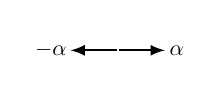
\begin{tikzpicture}[baseline=0]
     \draw[->,black,thick] (0.01,0) -- (0:0.6cm);
     \draw[->,black,thick] (-0.01,0) -- (180:0.6cm);
    \node[scale=0.8] at (-0.85,0) {$-\alpha$};
    \node[scale=0.8] at (0.75,0) {$\alpha$};
    \addvmargin{1mm}  
   \end{tikzpicture} & $\left(\begin{array}{c}2\end{array}\right)$ & \dynkin{A}{1}\\
$\mathsf{A}_1\times\mathsf{A}_1$ &  $0 $  & $0 $& $\frac{\pi}{2} $ & 未定 &  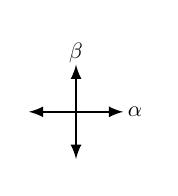
\begin{tikzpicture}[baseline=0]
    \foreach\ang in {0,90,180,270}{
     \draw[->,black,thick] (0,0) -- (\ang:0.6cm);}
    \node[scale=0.8] at (0.75,0) {$\alpha$};
    \node[scale=0.8] at (0,0.75) {$\beta$};
    \addvmargin{1mm}  
   \end{tikzpicture} & $\left(\begin{array}{cc} 2&0\\0&2\end{array}\right)$ & \dynkin{A}{1} \dynkin{A}{1}\\
 $\mathsf{A}_2$ &$-1 $  & $-1 $& $\frac{2\pi}{3} $ & 1 &
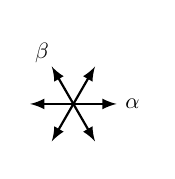
\begin{tikzpicture}[baseline=0]
    \foreach\ang in {0,60,...,300}{
     \draw[->,black,thick] (0,0) -- (\ang:0.55cm);}
    \node[scale=0.8] at (0.75,0) {$\alpha$};
    \node[scale=0.8] at (-0.4,0.65) {$\beta$};
    \addvmargin{1mm}
  \end{tikzpicture} & $\left(\begin{array}{cc} 2&-1\\-1&2\end{array}\right)$ & \dynkin{A}{2}\\
$\mathsf{B}_2$ &$-1 $  & $-2 $& $\frac{3\pi}{4} $ & 2 & 
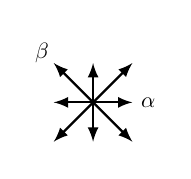
\begin{tikzpicture}[baseline=0]
    \foreach\ang in {0,90,180,270}{
     \draw[->,black,thick] (0,0) -- (\ang:0.5cm);}
    \foreach\ang in {45,135,225,315}{
     \draw[->,black,thick] (0,0) -- (\ang:0.70710678cm);}
    \node[scale=0.8] at (0.7,0) {$\alpha$};
    \node[scale=0.8] at (-0.65,0.63) {$\beta$};
    \addvmargin{1mm}
  \end{tikzpicture} & $\left(\begin{array}{cc} 2&-1\\-2&2\end{array}\right)$ & \dynkin{B}{2}\\
$\mathsf{G}_2$ &$-1 $  & $-3 $& $\frac{5\pi}{6} $ & 3 & 
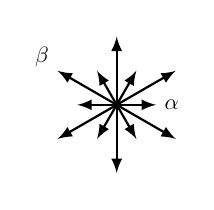
\begin{tikzpicture}[baseline=0]
    \foreach\ang in {0,60,...,300}{
     \draw[->,black,thick] (0,0) -- (\ang:0.5cm);}
    \foreach\ang in {30,90,...,330}{
     \draw[->,black,thick] (0,0) -- (\ang:0.8660254cm);}
    \node[scale=0.8] at (0.7,0) {$\alpha$};
    \node[scale=0.8] at (-0.95,0.61) {$\beta$};
    \addvmargin{1mm}
  \end{tikzpicture} & $\left(\begin{array}{cc} 2&-1\\-3&2\end{array}\right)$ & \dynkin{G}{2}\\
%五&$-1$  & $-1$ & $\frac{2\pi}{3}$ & 1\\
%六&$-1$  & $-2$ & $\frac{3\pi}{4}$ & 2\\
%七&$-1$  & $-3$ & $\frac{5\pi}{6}$ & 3\\
\hline
\end{tabular}
\end{table}


\begin{lemma}\label{9.2}
令$\Phi$为$\mathsf{E}$的一个根系统, 对应 Weyl 群$\mathscr{W}$. 若$\sigma\in GL(\mathsf{E})$保$\Phi$不变, 则对任何$\alpha\in \Phi$ 有$\sigma \sigma_{\alpha} \sigma^{-1} =\sigma_{\sigma(\alpha)}$, 且对所有$\alpha,\beta\in \Phi$, 有$\langle \beta,\alpha\rangle=\langle \sigma(\beta),\sigma(\alpha)\rangle$.
\end{lemma}

\begin{lemma}\label{9.4}设$\alpha$, $\beta$为线性无关的根. 若$(\alpha,\beta)>0$, 则$\alpha-\beta$为根. 若$(\alpha,\beta)<0$, 则$\alpha+\beta$为根.
\end{lemma}
\begin{proof}
第二个论断从第一个可得(只需作替换$\beta\rightarrow-\beta$). 由于$(\alpha,\beta)$与$\langle \alpha,\beta\rangle$同号, 故表\ref{t1}可见, 当它们都为正时, 总有$\langle \alpha,\beta\rangle$或$\langle \beta,\alpha\rangle$其中一者等于1. 若$\langle\alpha,\beta\rangle=1$, 则$\sigma_\beta(\alpha) = \alpha-\beta\in \Phi$; 否则若$\langle \beta,\alpha\rangle = 1$, 则$\beta-\alpha\in \Phi$, 从而$\alpha-\beta=\sigma_{\beta-\alpha}(\beta-\alpha)\in \Phi$. 即证.
\end{proof}

对线性无关的两个根$\alpha$, $\beta$, 考察所有形如经$\beta$处的$\alpha$-串$\beta+i\alpha$($i\in \mathbf{Z}$)的根: 设$r,q\in \mathbf{Z}^+$为使$\beta-r\alpha$, $\beta+q\alpha\in\Phi$的最大整数; 若某个$\beta+i\alpha\neq \Phi$ ($-r\leq i\leq q$), 则存在$p<s$使$\beta+p\alpha\in\Phi$, $\beta+(p+1)\neq \Phi$, $\beta+(s-1)\alpha\neq \Phi$, $\beta+s\alpha\in\Phi$, 从而由引理\ref{9.4}表明$(\alpha,\beta+p\alpha)>0$, $(\alpha,\beta+s\alpha)<0$, 但这与$p<s$矛盾(注意到$(\alpha,\alpha)>0$). 可见, \emph{经$\beta$处的$\alpha$-串从$\beta-r\alpha$到$\beta+q\alpha$是不间断的}. 因$\sigma_\alpha$作用在这些根上只是加上或减去若干$\alpha$的倍数, 故该$\alpha$-串在$\sigma_\alpha$下是不变的; 几何上来看显然$\sigma_\alpha$只是将该串收尾对调, 特别地$\sigma_\alpha(\beta+q\alpha) = \beta-r\alpha$, 故$\beta+q\alpha-\langle \beta+q\alpha,\alpha\rangle \alpha = \beta-r\alpha$, 即$\beta-\langle \beta,\alpha\rangle \alpha -q\alpha = \beta-r\alpha$, 从而$\langle \beta,\alpha\rangle = r-q$. 由于对于线性无关的两个根$\langle \beta,\alpha\rangle\leq3$, 故$r-q\leq 3$. 由于根串的节点个数为$r-q+1$, 故可见: \emph{根串的长度最多为4}.

$\Phi$的子集$\Delta$称为$\Phi$的一组基, 若满足如下条件:

(B1) $\Delta$ 是$\mathsf{E}$的一组基,

(B2) 任何根$\beta$都可写为$\beta=\sum k_\alpha \alpha$ ($\alpha\in \Delta$), 且系数$k_\alpha$均为非负整数和均为非正整数.

$\Delta$中的根称为\textbf{单根}. 由(B1)知$\mathrm{Card}\,\Delta = \ell$且$\beta$在$\Delta$上的展开系数是唯一的. 从而可以定义一个根(相对于$\Delta$)的\textbf{高度}: $\mathrm{ht}\,\beta = \sum_{\alpha\in\Delta} k_\alpha$. 若所有$k_\alpha \geq0$ ($k_\alpha\leq 0$), 则称$\beta$为正(负), 记为$\beta \succ 0$($\beta\prec 0$). 正, 负根(相对于$\Delta$)的集合记为$\Phi^+$和$\Phi^{-}$ (有$\Phi^-=-\Phi^+$). 若$\alpha$和$\beta$均为正根, 且$\alpha+\beta$也为根, 则显然$\alpha+\beta$也为正根. 从而$\Delta$定义了$\mathsf{E}$上的一个偏序: 定义$\mu\prec \lambda$ 若$\lambda-\mu$为正根之和或$\mu=\lambda$. $\Delta$的定义未保证其存在性, 其存在性将由定理\ref{10.1}保证.
\begin{lemma}\label{10.1l}
若$\Delta$为$\Phi$的基, 则对$\alpha \neq \beta \in \Delta$, 有$(\alpha,\beta)\leq 0$, 且$\alpha-\beta$不为根.
\end{lemma}
\begin{proof}
由基定义的(B2), 对任何$\alpha\neq \beta\in \Delta$, $\alpha-\beta$不能为根(因$\alpha,\beta\in\Delta$前的系数一正一负). 假设$(\alpha,\beta)>0$, 则由$\alpha\neq \beta$(假设), 且显然$\alpha \neq -\beta$, 故引理\ref{9.4}表明$\alpha-\beta$为根, 矛盾. 故只能$(\alpha,\beta)<0$.
\end{proof}



对任意$\mathsf{E}$中的向量$\gamma$, 定义$\Phi^+(\gamma) = \{\alpha\in \Phi|(\gamma,\alpha)>0\}$为那些与$\gamma$夹锐角的根的集合. 显然$\mathsf{E}-\cup_{\alpha \in\Phi} P_\alpha$非空, 故称$\gamma\in \mathsf{E}$为正常的, 若$\gamma\in \mathsf{E}-\cup_{\alpha \in\Phi} P_\alpha$, 否者称其为奇异的. 当$\gamma$为正常时,显然有$\Phi=\Phi^+(\gamma)\cup(-\Phi^\dag(\gamma))$. 称$\alpha\in\Phi^+(\gamma)$为可分解的, 若存在$\beta_1,\beta_2\in\Phi^+(\gamma)$使$\alpha=\beta_1+\beta_2$, ,否则称其为不可分解的. 有如下定理:

\begin{theorem} \label{10.1}设$\gamma\in\mathsf{E}$为正常的. 则所有$\Phi^+(\gamma)$中的所有不可分解根的集合, 记为$\Delta(\gamma)$, 为$\Phi$的一个基, 且任何基都可由此得到.
\end{theorem}

\begin{proof}
分如下步骤:

(1) $\Phi^+(\gamma)$中的每个根都为$\Delta(\gamma)$中向量的非负$\mathbf{Z}$线性组合. 否则, 存在$\alpha\in \Phi^+(\gamma)$不满足条件; 则选使得$(\gamma,\alpha)$尽可能小的$\alpha$. 显然$\alpha\notin \Delta(\gamma)$, 即$\alpha \in \Phi^+(\gamma)$不是不可分解根, 从而其为可分解根, 则按定义存在$\beta_1,\beta_2\in\Phi^+(\gamma)$使得$\alpha=\beta_1+\beta_2$, 故$(\gamma,\alpha)=(\gamma,\beta_1)+(\gamma,\beta_2)$. 但由$\Phi^+(\gamma)$定义每个$(\gamma,\beta_i)$都为正, 且比$(\gamma,\alpha)$小, 为了不与$\alpha$的选取矛盾, 故只能$\beta_1$和$\beta_2$都能写为$\Delta(\gamma)$中元素的非负$\mathbf{Z}$-线性组合, 但这也推出$\alpha$也可以, 仍与$\alpha$的选取矛盾.

(2) 若$\alpha,\beta\in\Delta(\gamma)$, 则$(\alpha,\beta)\leq 0$, 否则$\alpha=\beta$. (注意该命题与引理\ref{10.1l}的不同之处; 但证明类似.) 否则, $(\alpha,\beta)>0$, 从而由引理\ref{9.4}, $\alpha-\beta$为一个根. 由于显然$\beta\neq -\alpha$, 故$\alpha-\beta$或$\beta-\alpha$中有一者在$\Phi^+(\gamma)$中, 则利用$\alpha=\beta+(\alpha-\beta)$ 或$\beta=\alpha+(\beta-\alpha)$, 可见$\alpha$或$\beta$为可分解的, 与$\alpha$, $\beta$的选取矛盾.

(3) $\Delta(\gamma)$中的元素均线性独立. 设$\sum r_\alpha \alpha = 0$ ($\alpha\in \Delta
(\gamma)$, $r_\alpha\in\mathbf{R}$), 将系数$r_\alpha$分为大于零和小于零的两组得到$\sum s_\alpha \alpha = \sum t_\beta \beta$ (这里$s_\alpha,t_\alpha >0$, 且$\alpha$和$\beta$指标集不交), 并记等式两边都等于$\varepsilon$. 则根据(2), $(\varepsilon,\varepsilon) = \sum_{\alpha,\beta} s_\alpha t_\beta (\alpha,\beta) \leq 0$, 使得只能$\varepsilon=0$, 从而$0=(\gamma,\varepsilon) = \sum s_\alpha(\gamma,\alpha)$, 且$\alpha\in \Delta(\gamma)\subset \Phi^+(\gamma)$故$(\gamma,\alpha)>0$, 故所有$s_\alpha=0$; 同理所有$t_\beta=0$. (注: 这一部分事实上还证明了: 若有若干向量都处于某超平面$P_\gamma$的同一侧, 且它们两两夹钝角, 则它们必线性无关.)

(4) $\Delta(\gamma)$为$\Phi$的一个基. 由于$\Phi=\Phi^+(\gamma)\cup -\Phi^+(\gamma)$, (B2)已由(1)保证, 且由(1)知$\Delta(\gamma)$张成$\Phi^+(\gamma)$, 也即张成$\mathsf{E}$, 再由(3)知(B1)满足. 故$\Delta(\gamma)$为$\Phi$的一个基. 

(5)  $\Phi$的每个基$\Delta$都形如$\Delta(\gamma)$, 这里$\gamma\in \mathsf{E}$是某个正常向量. 给定$\Delta$, 选取$\gamma\in\mathsf{E}$使$(\gamma,\alpha)>0$ $\forall \alpha\in \Delta$(这总可以做到). 由(B2), $\gamma$为正常的, 且$\Phi^\pm \subset \pm \Phi^\pm(\gamma)$, 故只能有$\Phi^\pm = \pm \Phi^\pm(\gamma)$, $\Delta$显然只能由不可分解根构成(否则设$\alpha\in\Delta$为可分解根, 则有$\alpha=\beta_1+\beta_2$, 这里$\beta_1,\beta_2\in \Phi^+(\gamma) = \Phi^+$故都为正根, 但$\alpha$在$\Delta$上的展开是唯一的, 只能为$\alpha$, 矛盾), 从而$\Delta\subset \Delta(\gamma)$; 但有$\Delta=\mathrm{Card}\,\Delta(\gamma)=\ell$故$\Delta=\Delta(\gamma)$.
\end{proof}

%\begin{theorem}\label{10.1}
%$\Phi$总有一组基.
%\end{theorem}

$P_\alpha(\alpha\in\Phi)$将$\mathsf{E}$分为有限各区域: $\mathsf{E}-\cup_{\alpha \in\Phi} P_\alpha$中的连通分支称为$\mathsf{E}$的(开)\textbf{Weyl室}, 记为$\mathfrak{C}(\gamma)$. 式子$\mathfrak{C}(\gamma)=\mathfrak{C}(\gamma')$等价于说$\gamma$, $\gamma'$在超平面$P_\alpha(\alpha\in\Phi)$的同一侧. 可见Weyl室与基有自然的一一对应关系. 若$\Delta=\Delta(\gamma)$, 则记$\mathfrak{C}(\Delta)=\mathfrak{\gamma}$, 并称$\mathfrak{C}(\Delta)$为\textbf{相对于$\Delta$的基本Weyl室}.


\begin{theorem}\label{10.3}设$\Delta$为$\Phi$的一组基.

(a) 若$\gamma\in\mathsf{E}$, 则存在$\sigma\in\mathscr{W}$, 使$(\sigma(\gamma),\alpha)>0$对所有$\alpha\in \Delta$成立(故$\mathscr{W}$遍历地作用于Weyl室).

(b) 若$\Delta'$为$\Phi$的另一组基, 则存在$\sigma\in\mathscr{W}$使$\sigma(\Delta')=\Delta$(故$\mathscr{W}$遍历地作用于不同的基之间).

(c) 若$\alpha$为任何根, 则存在$\sigma\in\mathscr{W}$使$\sigma(\alpha)\in \Delta$.

(d) $\mathscr{W}$由$\sigma_\alpha$ ($\alpha\in\Delta$) 生成.

(e) 若$\sigma(\Delta)=\Delta$, $\sigma\in \mathscr{W}$, 则$\sigma=1$ (故$\mathscr{W}$在不同基间的作用是单遍历的).
\end{theorem}


称$\Phi$为\textbf{不可约的}, 若其不可能被划分为两个真子集的并, 满足第一个真子集中的任意向量都正交于第二个真子集中的任意向量. 有如下引理:
\begin{lemma}\label{10.4}
设$\Phi$不可约.

(a)在偏序$\prec$的意义下, 存在唯一的极大根$\beta$(特别地, 对所有$\alpha\in\Phi$, $\alpha\neq \beta$蕴含$\mathrm{ht}\,\alpha < \mathrm{ht}\,\beta$, 且$(\beta,\alpha)\geq 0$, $\forall \alpha \in \Delta)$. 若$\beta=\sum k_\alpha \alpha (\alpha\in \Delta)$, 则 所有$k_\alpha>0$.

(b)$\mathscr{W}$在$\mathsf{E}$上的作用不可约. 特别地, 一个根$\alpha$在$\mathscr{W}$作用下的轨道张成$\mathsf{E}$.

(c) $\Phi$中最多有两种根长(从而定义了长根和短根), 且所有有同一长度的根在$\mathscr{W}$下共轭.

(d) 唯一极大根$\beta$为长根.
\end{lemma}

选定单根的一组排序$(\alpha_1,...,\alpha_\ell)$, 则矩阵$(\langle \alpha_i,\alpha_j\rangle)$称为$\Phi$的\textbf{Cartan矩阵}, 其矩阵元称为\textbf{Cartan整数}.

\begin{proposition} 令$\Phi'\subset \mathsf{E}'$为另一个根系统, 其有一组基为$\Delta'=\{\alpha'_1,...,\alpha'_\ell\}$. 若$\langle \alpha_i,\alpha_j\rangle = \langle \alpha'_i,\alpha'_j\rangle$ 对$1\leq i,j\leq \ell$成立, 则双射$\alpha_i\mapsto \alpha'_i$可唯一地扩张到同构$\phi\colon\mathsf{E}\rightarrow\mathsf{E}'$, 且$\phi$将$\Phi$映到$\Phi'$, 且满足$\langle \phi(\alpha),\phi(\beta)\rangle = \langle \alpha,\beta\rangle$ 对任何$\alpha,\beta\in \Phi$成立. 从而, $\Phi$的Cartan矩阵(在相差一个同构的意义下)决定了$\Phi$.
\end{proposition}

\dynkin{A}{}

\dynkin{B}{}

\dynkin{C}{}

\dynkin{D}{}

\dynkin{E}{6}

\dynkin{E}{7}

\dynkin{E}{8}

\dynkin{F}{4}

\dynkin{G}{2}


\section{同构和共轭定理}

\begin{proposition} 设$L$为一个单李代数, $H$为$L$的一个极大环面子代数, $\Phi\subset H^*$为$L$相对于$H$的根的集合. 则$\Phi$为一个不可约根系统.
\end{proposition}

\begin{proof}否则, 有分解$\Phi=\Phi_1\cup \Phi_2$, 这里$\Phi_1$与$\Phi_2$正交. 若取$\alpha\in\Phi_1$, $\beta\in\Phi_2$, 则$(\alpha+\beta,\alpha)\neq 0$且$(\alpha+\beta,\beta)\neq 0$, 故$\alpha+\beta$不可能在$\Phi_1$或$\Phi_2$中, 故不可能为根, 从而由命题\ref{8.1p}, $[L_\alpha L_\beta]\subset L_{\alpha+\beta}=0$, 故对于$L$的由所有$L_\alpha$ ($\alpha\in \Phi_1$)生成的子代数$K$, 其中心化子包含所有的$L_\beta$ ($\beta\in\Phi_2$); 特别地, 由于$Z(L)=0$, 故$K$为$L$的一个真子代数. 并且$K$的正规化子包含所有$L_\alpha$ ($\alpha\in \Phi_1$), 故$K$的正规化子包含所有$L_\alpha$ ($\alpha\in \Phi$), 从而利用命题\ref{8.4}(f)($L$由根空间$L_\alpha$生成)知$K$的正规化子为$L$, 从而$K$为$L$的一个不为零的真理想, 与$L$为单矛盾.
\end{proof}

下面再考察$L$为任意半单李代数时的情况: 此时由定理\ref{5.2}, $L$可被唯一写为直和$L_1\oplus\cdots \oplus L_t$, 这里的$L_i$均为单理想. 若$H$为$L$的一个极大环面子代数, 则$H=H_1\oplus...H_t$, 这里$H_i=L_i\cap H$(见练习5.8). 显然每个$H_i$都为$L_i$的环面子代数, 且事实上也为极大环面的: 任何$L_i$的比$H_i$大的环面子代数自然地为$L$中的环面子代数, 将所有$H_j, j\neq i$正规化, 且与$H_j$生成一个$L$的比$H$大的环面子代数, 故矛盾. 下面令$\Phi_i$为$L_i$相对于$H_i$的在欧式空间$\mathsf{E}_i$中的根系统. 若$\alpha\in \Phi_i$, 则通过对$j\neq i$时补充定义$\alpha(H_j)=0$则可将$\alpha$视为$H$上的线性函数, 可见$\alpha$为$L$相对$H$的一个根, 且$L_\alpha \in L_i$. 另一方面, 若$\alpha \in \Phi$, 则存在某个$i$, $[H_iL_\alpha]\neq 0$ (否则$H$将$L_\alpha$中心化), 故$L_\alpha\subset L_i$, 故$\alpha|_{H_i}$为$L_i$的一个相对于$H_i$的根. 从而可见$\Phi$可分解为$\Phi_1\cup...\cup \Phi_t$, 对应$\mathsf{E}\cong \mathsf{E}_1\oplus...\oplus \mathsf{E}_t$. 从而证明了以下推论:

\begin{corollary}
设$L$为一个半单李代数, 有极大环面子代数$H$及根系统$\Phi$. 若$L=L_1\oplus...\oplus L_t$为$L$的单理想分解, 则$H_i=H\cap L_i$为$L_i$的极大环面子代数, 且对应的(不可约)根系统$\Phi_i$可自然地视为$\Phi$的子系统, 这里$\Phi=\Phi_1\cup...\cup\Phi_t$将$\Phi$分解为不可约部分.
\end{corollary}

一个李代数$L$的\textbf{Cartan子代数}(简称为$\mathsf{CSA}$)为$L$中的一个幂零子代数, 且满足其等于其在$L$中的正规化子. 注意这个定义并没有保证$\mathsf{CSA}$的存在性. 但若$L$为半单李代数($\mathrm{char}\, \mathsf{F}=0$), 则$L$的一个极大环面子代数$H$为阿贝尔的(从而为幂零的), 且$N_L(H)=H$ (因为$L=H+\coprod_{\alpha\in \Phi} L_\alpha$, 且对$\alpha\in\Phi$有$[H L_\alpha]=L_\alpha$). 因而对半单李代数, 其$\mathsf{CSA}$总存在.

有如下定理:
\begin{theorem}
令$H$为李代数$L$的一个子代数. 则$H$为$L$的一个$\mathsf{CSA}$当且仅当$H$为一个极小Engel子代数(特别地, $\mathsf{CSA}$存在).
\end{theorem}

\begin{corollary}
$L$为半单的($\mathrm{char}\,\mathsf{F}=0$). 则$L$的(若干)$\mathsf{CSA}$恰为$L$的(若干)极大环面子代数.
\end{corollary}

设$\mathsf{F}$为特征为0的代数闭域. 则我们将证明, 对$\mathsf{F}$上的任意李代数$L$, 其所有$\mathsf{CSA}$都在内自同态$\Int L$的意义下共轭, 这里内自同态$\Int L$为所有由形如$\exp \ad x$ 生成的自同态群, $x\in L$为$\ad$-幂零元. 对于$L$半单的情形, 这表明所有极大环面子代数都共轭, 从而$L$被任何一个极大环面子代数的根系统完全确定(至多差一个同构). 注意这里$\mathsf{F}$为特征为零的代数闭域这一条件是关键的, 为利用这一定理, 我们常选$\mathsf{F}$为复数域$\mathbf{C}$而不选实数域$\mathbf{R}$.

\section{泛包络代数}

本节中对$\mathsf{F}$不作限制. 引入泛包络代数的概念, 是为了给任何$\mathsf{F}$上的李代数$L$配备一个含单位元1的结合代数(以后称为单位结合代数); ``泛''的意思是说这个结合代数是与$L$的交换子结构适配的``最大''代数.

选定一个$\mathsf{F}$上的有限维向量空间$V$. 定义$T^0V=\mathsf{F}$, $T^1V=V$, $T^2V=V\otimes V$,...,$T^mV= V\otimes\cdots\otimes V$(乘$m$次). 定义$\mathfrak{T}(V)=\coprod_{i=0}^\infty T^iV$并定义结合乘法: 对$\mathfrak{T}(V)$上的生成元(均为$V$的基的张量组合的形式)有$(v_1\otimes \cdots v_k)(w_1\otimes\cdots w_m) = v_1\otimes\cdots\otimes v_k \otimes w_1\otimes\cdots \otimes w_m\in T^{k+m}V$. 这样$\mathfrak{T}(V)$称为一个单位结合分级代数, 其由$1\in\mathsf{F}$及$V$的任一组基生成. 称其为$V$上的\textbf{张量代数}. $\mathfrak{T}(V)$在如下意义上为$n$个生成元($n=\dim V$)的泛结合代数: 给定任何$\mathsf{F}$-线性映射$\phi\colon V\rightarrow \mathfrak{U}$($\mathfrak{U}$是$\mathsf{F}$上具有单位元$1$的结合代数), 存在唯一的$\mathsf{F}$-代数的同态$\psi\colon \mathfrak{T}(V)\rightarrow \mathfrak{U}$, 满足$\psi(1)=1$,且使如下图交换($i$为嵌入映射):
$$
\xymatrix{ V\ar[dr]_\phi\ar[r]^i& \mathfrak{T}(V)\ar@{-->}[d]^{\exists \psi}\\
 & \mathfrak{U}}
$$
再令$I$为$\mathfrak{T}(V)$的由所有$x\otimes y-y\otimes x$生成的(双)理想, 称$\mathfrak{S}=\mathfrak{T}/I$为$V$上的对称代数, 记$\sigma\colon\mathcal{T}(V)\rightarrow\mathfrak{S}(V)$为自然映射. 注意到$I$的生成元在$T^2V$中, 故有$I=(I\cap T^2V)\oplus(I\cap T^3V)\oplus\cdots$. 从而$\sigma$在$T^0V=\mathsf{F}$和$T^1V=V$上为单射, 且$\mathfrak{S}(V)$从$\mathfrak{T}(V)$中继承了一个分级结构: $\mathfrak{S}(V)=\coprod_{i=0}^\infty S^iV$. 模掉$I$的作用就是使$V$中的元素交换, 故$\mathfrak{S}(V)$对于$V$到交换结合$\mathsf{F}$-代数(具有单位元1)的映射来说是泛交换结合代数. 且, 若固定$(x_1,...,x_n)$为$V$的一组基, 则$\mathfrak{S}(V)$与$\mathsf{F}$上的$n$变量多项式代数自然同构, 基为$1$和所有形如$x_{i(1)}...x_{i(t)}$, 这里$t\geq 1$, $1\leq i(1)\leq ...\leq i(t)\leq n$. 对无限维的$V$, 这样构造的$\mathfrak{T}(V)$和$\mathfrak{S}(V)$仍然有效.

对任意李代数$L$(可以为无限维), $L$的\textbf{泛包络代数}为$(\mathfrak{U},i)$, 这里$\mathfrak{U}$为$\mathsf{F}$上的一个单位结合代数(以后称为, $i\colon L\rightarrow\mathfrak{U}$为一个线性映射, 满足对任意$x,y\in L$, 有$i([xy])=i(x)i(y)-i(y)i(x)$. 这样定义的泛包络代数有如下范畴性质: 对任何单位结合$\mathsf{F}$-代数$\mathfrak{U}'$及任何满足上式的线性映射$j\colon L\rightarrow \mathfrak{U}'$, 存在唯一的代数单位同态$\phi\colon \mathfrak{U}\rightarrow \mathfrak{U}'$(单位同态意为$1\rightarrow 1$), 满足$\phi\circ i = j$. 为证该性质, 要证明唯一性和存在性; 在存在性中定义了$\mathfrak{U}(L)=\mathfrak{T}(L)/J$, 并记$\pi\colon \mathfrak{T}(L)\rightarrow \mathfrak{U}(L)$为自然映射. 

现定义$\mathfrak{T}=\mathfrak{T}(L)$, $\mathfrak{S}=\mathfrak{S}(L)$, $\mathfrak{U}=\mathfrak{U}(L)$, $T^m=T^m(L)$, $S^m=S^m(L)$. 定义$T_m=T^0\oplus T^1\oplus\cdots \oplus T^m$, 且定义$U_m=\pi(T_m)$, $U_{-1}=0$. 则有$U_mU_p\subset U_{m+p}$, $U_m\subset U_{m+1}$. 令$G^m=U_m/U_{m-1}$, $\mathfrak{U}$中乘法定义了双线性映射$G^m\times G^p\rightarrow G^{m+p}$, 可将此扩张为映射$\mathfrak{G}\times \mathfrak{G}\rightarrow \mathfrak{G}$, $\mathfrak{G} = \coprod_{m=0}^\infty G^m$, 从而$\mathfrak{G}$为一个单位分级结合代数.


\begin{theorem} (Poincar\'e-Birkhoff-Witt定理, 简称$\mathsf{PBW}$定理)映射$\omega\colon \mathfrak{S}\rightarrow \mathfrak{G}$为代数同构.
\end{theorem}


\section{权的抽象理论与表示论}

本节中$L$总表示一个(特征为零的代数闭域$\mathsf{F}$上的)半单李代数, $H$是一个选定的$L$的$\mathsf{CSA}$, $\Phi$为对应的根系统, $\Delta=\{\alpha_1,...,\alpha_\ell\}$为$\Phi$的一组基, $\mathscr{W}$为Weyl群. 本节研究对象为有限维$L$-模. 



在$\mathfrak{sl}(2,\mathsf{F})$的表示一节中, 我们定义了权和权空间的概念: 设$V$为一个有限维$\mathfrak{sl}(2,\mathsf{F})$-模, $h$为$\mathfrak{sl}(2,\mathsf{F})$中的(唯一的)半单元, 则$h$在$V$上的表示是对角的(即存在一组$V$的基使$h$在其上为对角矩阵), 则可利用$h$的特征值为$V$作直和分解. 更一般地, 对任意一个半单李代数, 若$V$为一个有限维$L$-模, 可利用$L$半单元的子代数(即极大环面子代数$H$)在$V$上的对角作用(由推论\ref{6.4c}保证)来对$V$作直和分解: $V=\coprod V_\lambda$, 这里$\lambda \in H^*$, $V_\lambda = \{v\in V| h.v=\lambda(h)v\,\, \forall h\in H\}$. 对任意$V$(有限或无限维), 子空间$V_\lambda$仍然可以有定义; 当$V_\lambda \neq 0$, 就称其为一个\textbf{权空间}, 并称$\lambda$为一个$V$的\textbf{权}(更准确地, 称为一个$H$在$V$上的权). \emph{简而言之, 权空间与权就是李代数的半单元(的集合)对空间$V$所作的直和分解及所记的指标(即半单元的特征值).} 举例: 将$L$看作它自身的模($L$通过诱导表示作用在自身$L$上, 使其成为$L$-模), 则权的集合就是所有根$\alpha \in\Phi$(对应的权空间为$L_\alpha$, 均为1维)外加$0$(对应权空间为$H$, 维度为$\ell$); 再如, 在研究$L=\mathfrak{sl}(2,\mathsf{F})$时, $H$上的线性函数$\lambda$完全由其在基向量$h$上的值$\lambda(h)$确定, 故$\lambda(h)=\lambda$只是一个数. 注意, 若$\dim V=\infty$, 则无法保证$V$为其所有权空间的和; 但所有权空间$V_\lambda$的和, 记为$V'$, 为直和(此源于对一个线性变换, 属于不同特征值的特征值线性无关). 且$V'$为$V$的一个$L$-子模: 若$x\in L_\alpha$, $v\in V_\lambda$, $h\in H$, 则$h.x.v=x.h.v+[hx].v= x.(\lambda(h)v)+(\alpha(h)x).v = (\lambda(h)+\alpha(h))x.v$, 故$L_\alpha$将$V_\lambda$映到$V_{\lambda+\alpha}$. 总结即得如下引理:
\begin{lemma}
设$V$为任意$L$-模. 则:

(a) $L_\alpha$将$V_\lambda$映到$V_{\lambda+\alpha}$ ($\lambda\in H^*$, $\alpha \in\Phi$).

(b) 和$V'=\sum_{\lambda\in H^*} V_\lambda$为直和, 且$V'$为$V$的一个$L$-子模.

(c) 若$\dim V< \infty$, 则$V=V'$.
\end{lemma}

一个$L$-模$V$中的(具有权$\lambda$的)\textbf{极大向量}为一个非零向量$v^+\in V_\lambda$, 其被所有的$L_\alpha$零化($\alpha\succ 0$, 或$\alpha\in \Delta$). 如此定义的$v^+$当然取决于$\Phi$的基$\Delta$的选取. (例如: 若$L$为单, $\beta$为$\Phi$中的相对于$\Delta$的极大根(见引理\ref{10.4}), 则任何$L_\beta$的非零元为$L$诱导表示的极大向量(由命题\ref{8.1p}有$[L_\beta L_\alpha]\subset L_{\alpha+\beta}$, 但因$\beta$为极大根, 故$\mathrm{ht}\, \beta$最大, 故对$\alpha\succ 0$, 只能$\alpha+\beta$不为根, 即$L_{\alpha+\beta}=0$). 

为了研究有限维不可约$L$-模, 先考察一类由极大向量生成的$L$-模, 定义如下: 若$L$-模$V$满足对一个极大向量$v^+\in V$(其权为$\lambda$)有$V=\mathfrak{U}(L).v^+$($\mathfrak{U}(L)$为$L$的泛包络代数), 则称$V$为\textbf{标准循环的}(具有权$\lambda$), 且称$\lambda$为$V$的\textbf{最高权}. 这样的$L$-模的结构是容易刻画的: 为此定义非零$x_\alpha \in L_\alpha$($\alpha\succ 0$), 且选取(唯一的)$y_\alpha\in L_{-\alpha}$满足$[x_\alpha y_\alpha]=h_\alpha$. 回忆: 对$\lambda,\mu\in H^*$, 偏序$\lambda\succ \mu$ 当且仅当$\lambda-\mu$可写为正根直和. 有如下定理:
\begin{theorem}\label{20.2} 令$V$为一个标准循环$L$-模, 其有极大向量$v^+\in V_\lambda$. 令$\Phi^+=\{\beta_1,...,\beta_m\}$, 则有:

(a) $V$由向量$y^{i_1}_{\beta_1}...y^{i_m}_{\beta_m}. v^+$($i_j\in \mathbf{Z}^+$)张成; 特别地, $V$可写为其权空间的直和.

(b) $V$的权空间都形如$\mu=\lambda - \sum_{i=1}^{\ell} k_i\alpha_i$ ($k_i\in \mathbf{Z}^+$), 即所有的权满足$\mu \prec \lambda$.

(c) 对每个$\mu\in H^*$, $\dim V_\mu<\infty$, 且$\dim V_\lambda = 1$.

(d) $V$的每个子模都可写为$V$的权空间的直和.

(e) $V$为不可分解$L$-模, 且有唯一极大(真)子模, 以及唯一对应的不可约商模.

(f) 任何一个$V$的非零同态像都为标准循环模, 具有权$\lambda$.
\end{theorem}

\begin{corollary} 设$V$为定理\ref{20.2}中的$V$. 进一步设$V$为不可约$L$-模, 则$v^+$(在相差一个非零数乘的意义下)为$V$的唯一极大向量.
\end{corollary}

\begin{theorem}\label{20.3A} 令$V$, $W$, 为具有最高权$\lambda$的标准循环模, 若$V$和$W$均不可约, 则它们同构.
\end{theorem}

如何构造标准循环模? 这里给出一个诱导模的构造: 一个标准循环模, 当看作一个$B$-模时($B$为Borel子代数: $B(\Delta) = H+\coprod_{\alpha \succ 0} L_\alpha$), 含有一个由给定最大向量生成的一维子模. 故我们选$v^+$为基生成一维向量空间$D_\lambda$,  定义$B$在$D_\lambda$上的作用: 对给定的$\lambda\in H^*$, $(h+\sum_{\alpha \succ 0} x_\alpha).v^+ = h.v^+=\lambda(h) v^+$. (验证$D_\lambda$为一个$B$-模; $D_\lambda$也为$\mathfrak{U}(B)$-模, 故可定义张量基$Z(\lambda) = \mathfrak{U}(L)\otimes_{\mathfrak{U}(B)}D_\lambda$, 其在$\mathfrak{U}(L)$的自然左作用下变为一个$\mathfrak{U}(L)$-模.)

现论断$Z(\lambda)$为具有权$\lambda$的标准循环模. 一方面, $Z(\lambda)$由$1\otimes v^+$生成. 另一方面, $1\otimes v^+$非零, 因$\mathfrak{U}(L)$为自由$\mathfrak{U}(B)$-模(定理17.3), 其基含有$1$即所有单项式$y^{i_1}_{\beta_1}...y^{i_m}_{\beta_m}$, 故$1\otimes v^+$为一个权为$\lambda$的最大向量. 

这样, 若$N^-=\coprod_{\alpha\prec 0} L_\alpha$, 则$Z(\lambda)$, 看作$\mathfrak{U}(N^-)$-模, 与$\mathfrak{U}(N^-)$同构. 更准确地, $\mathfrak{U}(L)\cong \mathfrak{U}(N^-)\otimes \mathfrak{U}(B)$ ($\mathsf{PBW}$定理), 故$Z(\lambda) \cong \mathfrak{U}(N^-)\otimes \mathsf{F}$. 

\begin{theorem}{20.3B}设$\lambda\in H^*$. 则存在权为$\lambda$的不可约标准循环模$V(\lambda)$.
\end{theorem}
\begin{proof}
$Z(\lambda)$(构造见上)为权$\lambda$的标准循环模, 且有唯一极大子模$Y(\lambda)$(定理\ref{20.2}(d), 故$V(\lambda)=Z(\lambda)/Y(\lambda)$为权$\lambda$不可约的标准循环模(定理\ref{20.2}(e)).
\end{proof} 

设$V$为一个有限维不可约$L$-模, 则$V$至少含有一个极大向量, 对应唯一确定的权$\lambda$, 且$V$的由此极大向量生成的子模必为$V$本身(由不可约性), 从而由定理\ref{20.3A}和\ref{20.3B}, $V$同构于$V(\lambda)$.

对每个单根$\alpha_i$, 记$S_i(=S_{\alpha_i})$为$L$中对应$\mathfrak{sl}(2,\mathsf{F})$的拷贝. 则$V(\lambda)$也为(有限维)$S_i$-模, 且$L$的极大向量也为$S_i$的极大向量. 特别地, 因存在权$\lambda$的极大向量, 则$\mathsf{CSA}$ $H_i\subset S_i$的权完全由标量$\lambda(h_i)$ ($h_i=_{\alpha_i}$)确定, 而由定理\ref{7.2}, 这要求$\lambda(h_i)$为一个非负整数. 故有如下定理:

\begin{theorem}
若$V$为一个有限维不可约$L$-模, 其最高权$\lambda$, 则$\lambda(h_i)$为一个非负整数($1\leq i\leq \ell$).
\end{theorem}
更进一步, 从定理\ref{7.2}可知, 若$V$为有限维$L$-模, $\mu$为$V$的一个权, 则$\mu(h_i)=\langle \mu,\alpha_i\rangle \in \mathbf{Z}$, $1\leq i\leq \ell$. 这样, 表示论中的权的概念与如下定义的权可以等同:

令$\Lambda$为一个集合, 其含有所有$\lambda \in\mathsf{E}$, 满足$\langle \lambda,\alpha\rangle \in\mathbf{Z}$ ($\alpha\in\Phi$), 并称这样的$\lambda$为\textbf{权}. 由于$\langle\lambda,\alpha\rangle = 2(\lambda,\alpha)/(\alpha,\alpha)$线性依赖于$\lambda$, 故$\Lambda$为$\mathsf{E}$的一个子集, 且包含$\Phi$. 可以证明, $\lambda\in\Lambda$, 当且仅当$\langle \lambda,\alpha\rangle\in \mathbf{Z}$ $\forall \alpha\in\Delta$. 现定义\textbf{根格}为$\Lambda$的由$\Phi$生成的群, 并记为$\Lambda_r$. 注意$\Lambda_r$为$\mathsf{E}$中的\textbf{格}, 因其为$\mathsf{E}$中的一组$\mathbf{R}$-基(即任何单根集$\Delta$)的$\mathbf{Z}$-铺张. 对于给定的$\Delta\subset \Phi$, 定义$\lambda \in \Lambda$为\textbf{主权}(\textbf{强主权}), 如果所有的整数$\langle \lambda,\alpha\rangle$ ($\alpha\in\Delta$)均为非负(正). 定义$\Lambda^+$为所有主权构成的集合. 利用之前的语言, $\Lambda^+$为所有处于基本Weyl室$\mathfrak{C}(\Delta)$闭包中的权, 且$\Lambda \cap \mathfrak{C}(\Delta)$为所有强主权构成的集合.

$V(\lambda)$的最高权$\lambda$为主权; 线性函数$\lambda$, 若使得所有$\lambda(h_i)$为(正)整数, 则成为(主)整的. 所有整线性函数故称为$H^*$中的一个格, 其包括根系统. 

定义记号: 若$V$为$L$-模, 则记$\Pi(V)$为所有权构成的集合; 对$V=V(\lambda)$, 则记为$\Pi(\lambda)$.


设$\Delta=\{\alpha_1,...,\alpha_\ell\}$, 则向量$2\alpha_i/(\alpha_i,\alpha_i)$构成$\mathsf{E}$的一组基. 定义$\lambda_1,...,\lambda_\ell$为(对于$\mathsf{E}$上内积的)对偶基: $\langle \lambda_i,\alpha_j\rangle = 2(\lambda_i,\alpha_j)/(\alpha_j,\alpha_j)=\delta_{ij}$. 由于所有$\langle \lambda_i,\alpha\rangle$ ($\alpha\in\Delta$)为非负整数, 故$\lambda_i$为主权. 称其为\textbf{(对于$\Delta$来说的)基本主权}.

\section{Chevalley基}

本节中$L$总表示一个(特征为零的代数闭域$\mathsf{F}$上的)半单李代数, $H$是一个选定的$L$的$\mathsf{CSA}$, $\Phi$为对应的根系统.

\begin{proposition} 设$\alpha$, $\beta$为线性无关的根, $\beta-r\alpha,...,\beta,...,\beta+q\alpha$为经$\beta$的$\alpha$-串. 则:

(a) $\langle\beta,\alpha\rangle=r-q$.

(b) 至多两种根长在串中出现.

(c) 若$\alpha+\beta\in \Phi$, 则$r+1=\frac{q(\alpha+\beta,\alpha+\beta)}{(\beta,\beta)}$.
\end{proposition}


\begin{lemma} 设$\alpha$, $\beta$为两线性独立根. 选$x_\alpha \in L_\alpha$, $x_{-\alpha}\in L_{-\alpha}$, 满足$[x_\alpha x_{-\alpha}] = h_\alpha$, 且选任意$x_\beta\in L_\beta$. 则如果$\beta-r\alpha,...,\beta+q\alpha$为经$\beta$的$\alpha$-串, 则由$[x_{-\alpha}[x_\alpha x_\beta]]=q(r+1)x_\beta$.
\end{lemma}

\begin{proposition}\label{25.2} 存在如下根向量$x_\alpha \in L_\alpha$ ($\alpha\in \Phi$)的选取:

(a) $[x_\alpha x_{-\alpha}] = h_\alpha$.

(b) 若$\alpha$, $\beta$, $\alpha+\beta\in\Phi$, $[x_\alpha x_\beta]=c_{\alpha\beta}x_{\alpha+\beta}$, 则$c_{\alpha\beta}=-c_{-\alpha,-\beta}$. 对任何这样选取的根向量, 标量$c_{\alpha\beta}(\alpha,\beta,\alpha+\beta \in\Phi)$自动满足:

(c) $c^2_{\alpha\beta} = q(r+1)\frac{(\alpha+\beta,\alpha+\beta)}{(\beta,\beta)}$, 这里$\beta-r\alpha,...,\beta+q\alpha$是经$\beta$处的$\alpha$-串.
\end{proposition}

由上方命题\ref{25.2}可以定义$L$的\textbf{Chevalley基}: 其为任何基$\{x_\alpha,\alpha\in\Phi; h_i,1\leq i\leq \ell\}$, 其中的$x_\alpha$满足\ref{25.2}中的(a)和(b), $h_i=h_{\alpha_i}$, $\Delta=\{\alpha_1,...,\alpha_\ell\}$为$\Phi$的一组基. 

\begin{theorem}\label{Chevalley}(Chevalley)令$\{x_\alpha,\alpha\in \Phi;h_i,1\leq i\leq \ell\}$为$L$的一组Chevalley基. 则结构常数都在$\mathbf{Z}$中. 更准确地, 我们有

(a) $[h_ih_j]=0$, $1\leq i,j\leq \ell$.

(b) $[h_ix_\alpha] = \langle \alpha,\alpha_i \rangle x_\alpha$, $1\leq i\leq \ell$, $\alpha\in\Phi$.

(c) $[x_\alpha x_{-\alpha}] = h_\alpha$ 为$h_1,...,h_\ell$的$\mathbf{Z}$-线性组合.

(d) 若$\alpha$, $\beta$为线性无关的根, $\beta-r\alpha,...,\beta+q\alpha$为经$\beta$处的$\alpha$-串, 则若$q=0$有$[x_\alpha x_\beta]=0$; 若$\alpha+\beta\in\Phi$有$[x_\alpha x_\beta]=\pm (r+1) x_{\alpha+\beta}$.
\end{theorem}

\section{仿射李代数}

根据Chevalley定理\ref{Chevalley}, 有限维单李代数完全由$3r$个生成元$\{E^i_\pm,H^i|i=1,...,r\}$及其关系刻画, 这些关系包括Jacobi恒等式及以下关系
$$[H^i,H^j]=0,\quad
[H^i,E^j_\pm] = \pm A^{ji} E^j_\pm,\quad[E^i_+,E^j_-] = \delta^{ij}H^j,\quad
(\ad E^i_\pm)^{1-A^{ji}}(E^j_\pm) =0\,\,(i\neq j),$$
其中$A$为Cartan矩阵, 即一个$r\times r$矩阵, 满足如下性质: 其为不可分解(意义为无论如何改变基的排列顺序也不能使$A$变为分块对角矩阵)且
$$A^{ii}=2,\quad A^{ij}\leq 0\,\,(i\neq j),\quad A^{ij}=0\Leftrightarrow A^{ji}=0,\quad A^{ij}\in \mathbb{Z},$$
且
$$\det A>0\quad \Leftrightarrow \quad\text{存在对角矩阵$D$和对称矩阵$S$满足$A=DS$, 且$S$为正定}.$$
对于单李代数, 由于Cartan矩阵完全决定了李代数, 故问题转化为对Cartan矩阵的分类. 现为了定义推广Cartan矩阵, 我们将最后一个条件推广为
$$\text{存在对角矩阵$D$和对称矩阵$S$满足$A=DS,$}$$
即去掉$S$正定的条件. 这时, 由Chevalley定理对应的李代数称为\textbf{Kac--Moody代数}. 特别地, 当$S$为半正定时, 称对应的李代数为\textbf{仿射型Kac--Moody代数}, 或称\textbf{仿射李代数}.

单李代数有平凡的中心, 而非单仿射李代数有非平凡中心: 定义
$$K:= \sum_{i=0}^r a^{\mathsf{v}}_i H^i,$$
则显然$[K,H^i]=0$, 且$[K,E^i_\pm] = \pm \sum_{j=0}^r a^{\mathsf{v}}_j A^{ij} E^i_\pm =0$, 这里$a^{\mathsf{v}}$定义为Cartan矩阵的(右)零向量, 满足$\sum_{j=0}^r A^{ij} a^{\mathsf{v}}_j=0$. 由定义, 仿射Cartan矩阵只有一个零特征值, 从而$\mathfrak{g}$的中心为一维, 即$K$是(最多差一个数乘)唯一的中心元. 

中心元的存在区别了非单仿射李代数与单李代数. 一般地, 对任何李代数$\mathfrak{g}$, 都可通过添加$\ell$个中心生成元$K^i$到$\mathfrak{g}$的生成元中, $[T^a,K^i]=0$, $i=1,...,\ell$, $a=1,...,d$, 从而构造了一个($\ell$-维)中心扩张$\hat{\mathfrak{g}}$; 这时原先的括号要推广到$[T^a,T^b]=f^{ab}{}_c T^c+f^{ab}{}_i K^i$, $f^{ab}{}_c$为$\mathfrak{g}$中的结构常数; 新的结构常数$f^{ab}{}_i$需要满足Jacobi恒等式, 故不能随意选取; 则$f^{ab}{}_i$的所有解的个数就决定了独立的中心扩张的个数. 对于直和的情形, $\hat{\mathfrak{g}} = \mathfrak{g}\oplus (u_1)^{\ell}$, $f^{ab}{}_i\equiv 0$显然为一个解, 但也可能有别的形式的解也对应此直和扩张: 记$\tilde{T}^a=T^a+u^a_iK^i$, 则由$[\tilde{T}^a,\tilde{T}^b]=[T^a,T^b]=f^{ab}{}_c T^c +f^{ab}{}_i K^i= f^{ab}{}_c (\tilde{T}^c-u^c_i K^i)+ f^{ab}{}_i K^i$, 且$[\tilde{T}^a,\tilde{T}^b] = \tilde{f}^{ab}{}_c\tilde{T}^c+\tilde{f}^{ab}{}_i K^i$, 知只需$\tilde{f}^{ab}{}_i = f^{ab}{}_i - \sum_c f^{ab}{}_c u^c_i = 0$. 即, 若记$[x,y]_{\text{new}}=[x,y]_{\text{old}} + \Omega(x,y)K$, 则要求$\Omega$为双线性反对称, 且满足$0=\Omega(x,[y,z])+\Omega(y,[z,x])+\Omega(z,[x,y])$, 即$\Omega$是一个2-cocycle. 中心扩张是平凡的, 当且仅当此cocycle也为一个coboundary, 即当且仅当$\Omega(x,y)$为$[x,y]_{\text{old}}$的线性函数. 

现限制$\mathfrak{g}$为一个复单李代数, 则存在一组基, 使得结构常数$f^{abc}$完全反对称, 且$\sum_a f^{abc}f^{abd}\propto \delta^{ab}$, 则Jacobi恒等式要求
$f^{ab}_i = \sum_{c,d,e} = f^{abc}f^{cde}f^{de}{}_i$, 故选取$u^a_i = \sum_{b,c} f^{abc} f^{bc}{}_i$可得$\tilde{f}^{ab}{}_i = \sum_{c,d,e} f^{abc}f^{cde}f^{de}{}_i-\sum_c f^{abc} u^a_i = 0$, 可见单(及半单)李代数无非平凡的中心扩张.


通过观察可知, 仿射李代数的Dynkin图中, 去掉任何一个节点, 将得到单李代数的Dynkin图. 通过$X_r^{(\ell)}$可区分两类非单仿射李代数, 即第一类($\ell=1$)和第二类($\ell >1$). 第一类中, 去掉零节点后得到相应单李代数的Dynkin图及正确的Coxeter记号, 但在第二类情形, Coxeter记号与相应单李代数Dynkin图的记号不同. 对任意仿射李代数$\mathfrak{g}=X^{(\ell)}_r$, 我们将对应的单李代数$X_r$记为$\mathfrak{g}_{\text{hor}}$, 称为$\mathfrak{g}$的水平子代数. 


我们已从Dynkin图猜到了单李代数和非单仿射李代数之间应有某种联系, 而上一段刚说明了单(及半单)李代数无平凡的中心扩张, 从而非单仿射李代数无法由单李代数直接作中心扩张得到. 接下来, 一个自然的思路是由单李代数$\bar{\mathfrak{g}}$出发, 得到某个推广的非单李代数$\bar{\mathfrak{g}}_{\text{generalized}}$, 而这个$\bar{\mathfrak{g}}_{\text{generalized}}$有非平凡的中心扩张. 这个思路事实上是可行的. 我们将看到, 这个推广的非单李代数(的一种选取方式)是圈代数$\bar{\mathfrak{g}}_{\text{loop}}$, 其为一个$\mathbb{Z}$-分级代数, 其0-级子空间$\bar{\mathfrak{g}}_{[0]}$为一个子代数, 且同构于单李代数$\bar{\mathfrak{g}}$. 再对圈代数$\bar{\mathfrak{g}}_{\text{loop}}$作中心扩张可得到仿射李代数.



对任何单李代数$\bar{\mathfrak{g}}$, 考察从$S^1$到$\bar{\mathfrak{g}}$的解析映射构成的向量空间. 若$\{T^a|a=1,...,d\}$为$\bar{\mathfrak{g}}$的一个基, $S^1$看作复平面(坐标用$z$表示)的单位圆, 则该向量空间的一组基为$\mathcal{B}=\{T^a_n|a=1,...,d; n\in \mathbb{Z}\}$, 这里$T^a_n:=T^a\otimes z^n$, $\otimes$为一个形式乘号. 在该空间上可自然地定义括号:
$$[T^a_m, T^b_n] \equiv [T^a\otimes z^m, T^b\otimes z^n]:=[T^a,T^b]\otimes(z^m\cdot z^n),$$
即
$$[T^a_m,T^b_n]=f^{ab}{}_cT^c \otimes z^{m+n} = f^{ab}{}_c T^c_{m+n}.$$
可以验证, 在该括号下, $S^1\rightarrow \bar{\mathfrak{g}}$的解析映射空间成为一个(无限维)李代数, 称为$\bar{\mathfrak{g}}$上的圈代数$\bar{\mathfrak{g}}_{\text{loop}}$. 因在李括号下$T^a_n$中的指标$n$为加性的(从而赋予李代数$\bar{\mathfrak{g}}_{\text{loop}}$以$\mathbb{Z}$-分级), 故$\bar{\mathfrak{g}}_{\text{loop}}$的由$T^a_0$生成的子集为一个子代数, 称为$\bar{\mathfrak{g}}_{\text{loop}}$的零模子代数, 记为$\bar{\mathfrak{g}}_{[0]}$.

现找出$\bar{\mathfrak{g}}_{\text{loop}}$的中心扩张: 可尝试
$$[T^a_m, T^b_n]=f^{ab}{}_cT^c_{m+n}+(f^{ab}{}_i)_{mn}K^i,$$
显然零模子代数$\bar{\mathfrak{g}}_{[0]}$与单李代数$\bar{\mathfrak{g}}$同构, 故通过对生成元的选取, 可令$(f^{ab}_i)_{00}=0$; 事实上可令$(f^{ab}_i)_{m0}=0$, $m\in\mathbb{Z}$. 从而, 对任何固定的$n$, 有$[T^a_n,T^b_0]=f^{ab}{}_c T^c_n$, 说明集合$\{T^a_n|a=1,...,d\}$在$\bar{\mathfrak{g}}_{[0]}$的诱导表示下变换, 且对指标$a,b$, 结构常数$(f^{ab}{}_i)_{mn}$构成$\bar{\mathfrak{g}}_{[0]}$的诱导表示的不变张量; 但(在相差数乘的意义下)只有一个这样的张量, 为$\bar{\mathfrak{g}}\cong \bar{\mathfrak{g}}_{[0]}$的Killing 型 $\bar{\kappa}$, 故只能有$\bar{\mathfrak{g}}_{\text{loop}}$的一维非平凡中心扩张, 即指标$i$可省去, 且有
$$(f^{ab})_{mn} = \bar{\kappa}^{ab} f_{mn}.$$
由于Killing型的对称性, $f_{mn}$必关于$m,n$反对称. 但已知$f_{m0}=0$ $\forall m\in \mathbb{Z}$. 事实上(turns out)只有一种可能: $f_{mn}=m\delta_{m+n,0}$. 总结可得, 存在唯一的$\bar{\mathfrak{g}}_{\text{loop}}$的非平凡中心扩张$\hat{\mathfrak{g}}$, 满足
$$[T^a_m,T^b_n]=f^{ab}{}_c T^c_{m+n}+m\delta _{m+n,0} \bar{\kappa}^{ab} K,$$
$$[K,T^a_n]=0.$$
若将$\hat{\mathfrak{g}}$的元素写为$x\otimes \mathcal{P}(z)+\zeta K$, 这里$x\in \bar{\mathfrak{g}}$, $\mathcal{P}$为一个Laurent多项式, 则任意两个$\hat{\mathfrak{g}}$中元的李括号写为
\begin{equation}
\begin{aligned}
{}[x\otimes \mathcal{P}(z)+\zeta K,y\otimes \mathcal{Q}(z)+\eta K]
&=
[x\otimes \mathcal{P}(z),y\otimes \mathcal{Q}(z)]\\
&=[ p^a_m T^a_m,q^b_n T^b_n]\\
&= p^a_m q^b_n (f^{ab}{}_c T^c_{m+n} + m \delta_{m+n,0}\bar{\kappa}^{ab} K\\
&= p^a_m q^b_n (f^{ab}{}_c T^c_{m+n} + (p^a_m q^b_{-m}\bar{\kappa}^{ab})m\\
&=[x,y]\otimes(\mathcal{P}(z)\mathcal{Q}(z))+\bar{\kappa}(x,y)K\otimes \Res(\mathcal{Q}(z)\partial \mathcal{P}(z)),
\end{aligned}
\end{equation}
我们感兴趣的$\bar{\mathfrak{g}}$通常为紧致实李代数. 这时可选一组基使$\bar{\kappa}^{ab} = -\delta^{ab}$, 则有
$$[T^a_m,T^b_n]=f^{abc}T^c_{m+n}-m\delta^{ab}\delta_{m+n,0}K.$$
如上构造的(复)李代数$\hat{\mathfrak{g}}$可写为
$$\hat{\mathfrak{g}}:= \bar{\mathfrak{g}}_{\text{loop}}\oplus\mathbb{C}K,$$
这里的和$\oplus$为半直和, 而
$$\bar{\mathfrak{g}}_{\text{loop}}:=\mathbb{C}[z,z^{-1}]\otimes_{\mathbb{C}} \bar{\mathfrak{g}}.$$
由对仿射李代数的根系统的构造, 可知第一类仿射李代数$\mathfrak{g}^{(1)}$由$\hat{\mathfrak{g}}$再添加一个生成元$D$得到:
$$\mathfrak{g}^{(1)} = \hat{\mathfrak{g}}\oplus \mathbb{C} D = \mathbb{C}[z,z^{-1}]\otimes_{\mathbb{C}} \bar{\mathfrak{g}}\oplus \mathbb{C}K\oplus \mathbb{C} D,$$
新的李括号定义为
$$[D,T^a_m]=-[T^a_m,D]=m T^a_m,\qquad [D,K]=0,$$
这样反对称性和Jacobi恒等式仍然成立.


$\bar{\mathfrak{g}}_{\text{loop}}$的零模子代数仍为$\hat{\mathfrak{g}}$的零模子代数, 可视为由那些与$D$交换的$T^a_m$生成, 且与有限维$\bar{\mathfrak{g}}$同构, 且与$\mathfrak{g}_{\text{hor}}$同构. 有 $\hat{\mathfrak{g}}_{\text{loop}} = [\mathfrak{g}^{(1)},\mathfrak{g}^{(1)}]$, 即$D$是唯一不出现在任何李括号右边的生成元. 从而称$D$为$g^{(1)}$的导子: 在子代数$\bar{\mathfrak{g}}_{\text{loop}}$上, $D$的作用如同$z d/dz$:
$$[D,x\otimes \mathcal{P}(z)] = x\otimes z\partial \mathcal{P}(z).$$

总结如下: 为从单李代数$\bar{\mathfrak{g}}$得到第一类仿射李代数$\mathfrak{g}^{(1)}$, 构造过程为
$$\bar{\mathfrak{g}}\rightarrow \bar{\mathfrak{g}}_{\text{loop}} \rightarrow \hat{\mathfrak{g}} \rightarrow \mathfrak{g}^{(1)}.$$


如上得到的只是第一类仿射李代数. 为得到第二类仿射李代数, 需要放宽$S^1$到$\bar{\mathfrak{g}}$的映射为解析的这一条件, 即不再要求$\mathcal{P}(e^{2\pi i}z)=\mathcal{P}(z)$, 而是对$x\in \bar{\mathfrak{g}}$引入扭转边界条件
$$x\otimes \mathcal{P}(e^{2\pi i} z)=\omega(x)\otimes\mathcal{P}(z),$$
这里$\omega$为$\bar{\mathfrak{g}}$的有限阶同态. 这样引入了$\bar{\mathfrak{g}}$的$\mathbb{Z}_\ell$-分级($\ell$为$\omega$的阶):
$\bar{\mathfrak{g}} = \bigoplus_{i=0}^{\ell-1} \bar{\mathfrak{g}}_{[i]}$, $\bar{\mathfrak{g}}_{[j]} :=\{x\in \bar{\mathfrak{g}}
|\omega(x) = e^{2\pi i\cdot j/\ell} x\}$, 且$[\bar{\mathfrak{g}}_{[i]},\bar{\mathfrak{g}}_{[j]}]\subseteq \bar{\mathfrak{g}}_{[i+j\mod \ell]}$. 这里$\bar{\mathfrak{g}}_{[0]}$为$\bar{\mathfrak{g}}$的一个子代数, 而$\bar{\mathfrak{g}}_{[j]}$, $j=1,...,\ell-1$按$\bar{\mathfrak{g}}_{[0]}$的某个最高权表示变换. $\bar{\mathfrak{g}}_{[j]}$的定义表明$\mathcal{P}$需满足
$$\mathcal{P}(e^{2\pi i} z) = e^{2\pi i\cdot j/\ell} \mathcal{P}(z).$$
与$x\in\bar{\mathfrak{g}}_{[j]}$相乘, 得到向量空间的一个基为
$$\{T^a_{m+j/\ell}\} \equiv \{T^a\otimes z^{m+j/\ell}|T^a\in \bar{\mathfrak{g}}_{[j]},j=0,1,...,\ell-1;m\in\mathbb{Z}\}.$$
像第一类情形一样, 向量空间在上面的基下自然地继承了李代数结构:
$$[T^a_{m+j/\ell},T^b_{n+j'/\ell}] = f^{ab}{}_c T^c_{m+n+(j+j')/\ell},$$
且存在唯一的非平凡中心扩张, 其由$\{T^a_{m+j/\ell}\}$及一个中心元$K$生成, 满足
$$[T^a_{m+j/\ell},T^b_{n+j'/\ell}] = f^{ab}{}_c T^c_{m+n+(j+j')/\ell
} + \left( m + \frac{j}{\ell}\right) \bar{\kappa}^{ab} \delta_{m+n+(j+j')/\ell,0} K$$
及$[T^a_{m+j/\ell},K]=0$. 将此李代数记为$\hat{\mathfrak{g}}^{\omega}$. 类似地, 可以找到一个导子$D$, 从而使得$D$扩张后的李代数为第二类李代数$\mathfrak{g}^{\omega} = \bar{\mathfrak{g}}\oplus \mathbb{C} D$.  总结如下:

$$\bar{\mathfrak{g}}\rightarrow \bar{\mathfrak{g}}_{\text{loop}} \rightarrow \hat{\mathfrak{g}}^{\omega} \rightarrow \mathfrak{g}^{\omega}.$$


在第一类仿射李代数中, $\mathfrak{g}_{\text{hor}}$与$\bar{\mathfrak{g}}$同构, 对第二类仿射李代数, 有 $\mathfrak{g}_{\text{hor}}\cong \bar{\mathfrak{g}}_{[0]}\subset \bar{\mathfrak{g}}$.

若放宽$\bar{\mathfrak{g}}$的条件使得其为可约$\bar{\mathfrak{g}}$, 则需对每个单李代数及每个$u_1$-子代数引入中心扩张, 但$u_1$的中心扩张可等价为一个, 因为$u_1$的不可约模都为一维的. 故若写$\bar{\mathfrak{g}}=\bar{\mathfrak{s}}\oplus \bar{\mathfrak{h}}$, 这里$\bar{\mathfrak{s}}$为半单, $\bar{\mathfrak{h}}$为阿贝尔, 则$\bar{\mathfrak{g}}_{\text{loop}}$的中心扩张有如下直和形式
$$\hat{\mathfrak{g}}=\hat{\mathfrak{s}}\oplus \hat{\mathfrak{h}},$$
这里$\bar{\mathfrak{s}}$如前, 而$\hat{\mathfrak{h}}$写为
\begin{equation}\label{tab}
[t^a_m,t^b_n] = d^{ab} m \delta_{m+n,0}K,
\end{equation}
这里$m,n\in \mathbb{Z}$, $a,b=1,...,\dim \bar{\mathfrak{h}}$, 且$d^{ab}$为常数对称矩阵. 这样的李代数称为Heisenberg代数. 任何仿射李代数含有Heisenberg代数为子代数, 即由$\{H^i_m\}$和$K$生成的, 满足$[H^i_m,K]=0$和$[H^i_m,H^j_n] = \bar{\kappa}(H^i,H^j)m\delta_{m+n,0}K$的代数. 若式\ref{tab}中无$a$指标时,  称为$\hat{u}_1$ Kac\--Moody代数. 注意, 适当重新定义生成元可将$d^{ab}$写为$\delta^{ab}$, 从而任何Heisenberg代数都同构于$\hat{u}_1$代数的直和. 



\section{共形场论}

我们为仿射李代数寻找一个生成函数. 回忆仿射李代数有生成元$T^a_m$, 满足
\begin{equation}\label{af}
[T^a_m,T^b_n] = f^{ab}{}_c T^c_{m+n} + m\bar{\kappa}^{ab} \delta_{m+n,0} K.
\end{equation}
定义
\begin{equation}\label{jt}
J^a(z):= \sum_{n\in \mathbb{Z}} T^a_n z^{-n-1},
\end{equation}
称为Affine current或current. 任何以$z$为宗量的量都将称为场, 或场算符.
显然, 有
\begin{equation}\label{tj}
T^a_m = \frac{1}{2\pi i} \oint_0 dz z^m J^a(z) = \Res_0 z^m J^a.
\end{equation}
%我们定义的$J^z(z)$需要与仿射李代数定义\ref{af}兼容. 而在展开时
%\begin{equation}
%\begin{aligned}
%[T^a_m,T^b_n] &= \frac{1}{2\pi i}\oint_0 dz \frac{1}{2\pi i}\oint_0 dw %z^m w^n[J^a(z),J^b(w)]\\
%&= \frac{1}{2\pi i}\oint_0 dz \frac{1}{2\pi i}\oint_0 dw z^m w^nJ^a(z)J^b(w)-J^b(w) J^a(z)
%\end{aligned}
%\end{equation}
式\ref{tj}和\ref{jt}可互推, 也并不会影响原先仿射李代数的定义式\ref{af}. 形式上, 这是因为将\ref{tj}带入式\ref{af}之后, 围道积分在李括号之内就已求值并得到$T^a_m$了, 这样一来\ref{af}也就成了恒等式. 现在, 我们考察能否将积分号提到括号外来, 即能否写
$$[T^a_m,T^b_n] = \frac{1}{2\pi i}\oint_0 dz \frac{1}{2\pi i}\oint_0 dw z^m w^n[J^a(z),J^b(w)]?
$$
注意到$[J^a(z),J^b(w)] = [\sum_{m\in \mathbb{Z}} T^a_m z^{-m-1},\sum_{n\in \mathbb{Z}} T^b_n w^{-n-1}] = \sum_{m,n\in \mathbb{Z}} z^{-m-1} w^{-n-1}[T^a_m,T^b_n]$, 求和号可以提到李括号外面来, 源于李括号的双线性. 这一李括号进而等于$\sum_{m,n\in \mathbb{Z}} z^{-m-1} w^{-n-1} (f^{ab}{}_c T^c_{m+n} + m \bar{\kappa}^{ab}\delta_{m+n,0}K) = \sum_{m\in \mathbb{Z}} (w/z)^{m+1} \sum_{l\in \mathbb{Z}} z^{-l-2}(f^{ab}{}_c T^c_l+m\bar{\kappa}^{ab}\delta_{l,0}K)=\sum_{m\in \mathbb{Z}} (w/z)^{m+1}(z^{-1} T^c(z)+m z^{-2}\bar{\kappa}^{ab}K)$, 若围道为$w,z\in \{z||z|=1\}=S^1$, 则对$m$的求和发散. 可见, 为能将积分号提到括号外, 必须改变积分围道.

我们作如下尝试: 若写
$$[T^a_m,T^b_n]=\frac{1}{2\pi i}\oint_0 dz \frac{1}{2\pi i}\left(
\oint_{C_1} dw z^m w^n J^a(z)J^b(w)-\oint_{C_2} dw z^m w^n J^b(w) J^a(z)\right),$$
对$J^b(W)$的积分是在围道$w\in C_1$和$w\in C_2$上. 现在定义一个新的函数, 记为$\mathcal{R}(J^a(z)J^b(w))$, 使其在$C_1\cup C_2$上与上式值相同:
$$[T^a_m,T^b_n] = \frac{1}{2\pi i}\oint_0 dz \frac{1}{2\pi i} \oint_{C_1\cup C_2} dw z^m w^n \mathcal{R}(J^a(z)J^b(w)),$$
配合定义
$$
\mathcal{R}(J^a(z)J^b(w))
:=\left\{\begin{array}{cc}
J^a(z)J^b(w)& w\in C_1(z) = \{w|\text{某逆时针围道, }|w|< |z|\}\\
J^b(w)J^a(z)& w\in C_2(z) = \{w|\text{某顺时针围道, }|w|> |z|\}\\
\end{array}\right.
$$
则事实上$\oint_{C_1\cup C_2} dw z^m w^n \mathcal{R}(J^a(z)J^b(w))$可改为
$\oint_{|w-z|=1/2} dw z^m w^n \mathcal{R}(J^a(z)J^b(w))$, 若有
$$\mathcal{R}(J^a(z)J^b(w))
=(z-w)^{-2}\bar{\kappa}^{ab}K-(z-w)^{-1} f^{ab}{}_c T^c(w)+\mathcal{O}(z-w)^0,$$
则
\begin{equation}
\begin{aligned}
{}[T^a_m,T^b_n] &= \frac{1}{2\pi i} \oint_0 dz \frac{1}{2\pi i} dw z^m w^n
[(z-w)^{-2}\bar{\kappa}^{ab}K-(z-w)^{-1} f^{ab}{}_c T^c(w)+\mathcal{O}(z-w)^0]\\
&= \frac{1}{2\pi i} \oint_0 dz z^m[[-(\frac{d}{dz}z^n)\bar{\kappa}^{ab} K + z^n f^{ab}{}_c T^c(z)+0]\\
&=-n\bar{\kappa}^{ab} \delta_{m+n,0}K + f^{ab}{}_c T^c_{m+n}.
\end{aligned}
\end{equation}


考察$d$维时空流形上的共形变换的无穷小作用, 得到一个$\frac{(d+1)(d+2)}{2}$-维的(非半单)李代数. 将时空紧致化后, 该李代数生成的共形群为$SO(d-2,2)$的一个覆盖. 对$d=2$, 无穷小作用恰为柯西--黎曼方程, 表明解为所有的解析函数$f(z)$和$\bar{f}(\bar{z})$(两者独立), 则有限共形变换构成一个无限维李群, 其为全纯和反全纯坐标变换的直和. 考虑全纯函数, 选生成元$L^{(c)}_n = - z^{n+1}\frac{d}{dz}$, 则有$[L^{(c)}_m,L^{(c)}_n] = (m-n) L^{(c)}_{m+n}$,称为Witt代数. 这里上标``$(c)$''表``经典''; Witt代数在量子化时变为Virasoro代数$\mathcal{V}$(由L\"{u}axgwe--Mach定理保证). 量子场生成Hilbert空间, 而Hilbert空间为李代数的模, 从而可视场算符的集合为一个$\varphi(z,\bar{z})$为$\mathcal{V}\oplus \mathcal{V}$-模. 同时, 场的编序乘积定义为其算符展开:
$$\varphi_i(z,\bar{z})\varphi_j(w,\bar{w})=\sum_k d_{ij}{}^k(z,\bar{z},w,\bar{w})\varphi_k(w,\bar{w}),$$
称为共形场论的算符积代数.

$L_0+\bar{L}_0$生成伸缩变换, 故若将径向编序与编时等同, 则该算符扮演能量算符的角色, 故其能谱有最小值, 从而对应场$\varphi$的Virasoro-模为$\mathcal{V}$和$\bar{\mathcal{V}}$共同的最高权模; 其中最高权向量对应的场算符称为初级场, 记为$\phi(z,\bar{z}) \equiv \phi_{c,\Delta;\bar{c},\bar{\Delta}}(z,\bar{z})$. 则有$L_n\phi=0$ 对$n>0$, $L_0\phi = \Delta \phi$, $L_{-1}\phi=-\partial \phi$($L_{-1}$可等同于$L^{(c)}_{-1} = -d/dz$; $L_0$类似). 从而
$$\phi(z,\bar{z}) \mapsto \phi(w,\bar{w}) \cdot \left(\frac{d w}{dz}\right)^\Delta \left( \frac{d \bar{w}}{d \bar{z}}\right)^{\bar{\Delta}}.$$
对应非最高权向量的场称为次级场(或初级场的衍生场).

只依赖于$z$(或$\bar{z}$)的场在算子代数下封闭, 称为对称代数; 其又为全纯和反全纯部分的直和, 分别称为手性代数. 一个自然的问题是用手性代数分类共形场. 当手性代数为Virasoro代数和一个仿射代数的半直和$\mathcal{V}\oplus \mathfrak{g}$时, 手性场为$T(z)$和$J(z)$. 这时初级场也对应仿射代数的最高权向量, 故(对第一类仿射代数)初级场$\phi\equiv \phi_\Lambda$满足$T^a_n\phi =0$, $T^a_0 \phi = T^a_{(\bar{\Lambda})}\phi$($T^a_{(\bar{\Lambda})} = R_{\bar{\Lambda}}(T^a)$. 中心生成元$K$的特征值(对任何场)都为$k$.


共形场论的融合规则: 任何两个初级场的乘积都可由(初级和次级)场展开, 得到的展开系数类似研究单李代数的Kronecker乘积时的Clebsch-Gordan系数; 另外我们知道次级场的展开系数由对称代数$\mathcal{W}$完全决定, 故经常我们只需要知道初级场的展开系数. 这可以形式地写为$\{\phi_i\}$, $\phi_i\ast \phi_j = \sum_k \mathcal{N}_{ij}{}^k \phi_k$. 这里的$\mathcal{N}_{ij}^k$类似于眼镜Kronecker乘积时引入的Littlewood-Richardson系数: $\bar{\Lambda}_i\times \bar{\Lambda}_j = \sum_k \mathcal{L}_{ij}{}^k \bar{\Lambda}_k$. 共形场论的自然性: 创算符的展开系数为零当且仅当融合系数为零. 

对称代数的最大扩张: 若其中只有有限个初级场, 则这样的共形场论称为有理型共形场论. 所有的WZW理论都为有理型的(因利用初级场可生成仿射李代数的最高权模, 这样的模有有限多个).



\section{Weinberg}

一个系统的所有对称操作构成群$G$. 考察这个系统中的量子态, Wigner定理保证对称操作在量子态上的作用是幺正或反幺正的. 对两个对称操作$g_1,g_2\in G$, 在一个量子态$|\psi\rangle$上的作用有两种写法$U(g_2)U(g_2)|\psi\rangle$和$U(g_2g_1)|\psi\rangle$, 两种写法允许差一个相位$e^{i\phi}$. 天然地, $\phi$应该与$g_1$, $g_2$, 及量子态$\psi$都有关系, 即记为$\phi_\psi(g_1,g_2)$; 但事实上$\phi$与所作用得量子态无关(为证此, 只需将$|\psi\rangle$写成两个线性无关的态的叠加$|\psi\rangle = |\psi_A\rangle +|\psi_B\rangle$, 就可推出$e^{\pm i\phi_{\psi}} |\psi\rangle = e^{\pm i \phi_{\psi_A}}|\psi_A\rangle+e^{\pm i \phi_{\psi_B}}|\psi_B\rangle$, 从而$e^{i\phi_{\psi}} = e^{i\phi_{\psi_A}} = e^{i\phi_{\psi_B}}$ 与态无关), 从而可写为$\phi(g_1,g_2)$. 从而$G$在量子态空间(即Hilbert空间)上的表示为射影表示. 若$G$为李群, 则$\phi$在单位元$\phi(1,1)$附近可写为$\phi(g_1(\theta_1),g_2(\theta_2)) = f_{ab} \theta^a_1 \theta^b_2$, 这里$g_1=\theta_1^a T^a$为李群单位元附近的展开. 从而对李代数$\mathfrak{g}$的效果为添加一项: $f^{ab}{}_c T^c\rightarrow f^{ab}{}_c T^c + f^{ab} 1$. 注意, 这里的$1$为李群的单位元, 本不在$\mathfrak{g}$中; 但可以形式地引入$K$, 其与$\mathfrak{g}$的元素均交换(从而扮演了上面的$1$的位置), 使得$\mathfrak{g}\oplus\mathbb{C} K$为一个新的李代数, 其在量子态上的(基本)表示正是$\mathfrak{g}$在量子态上的射影表示. 这样引入的新李代数称为对$\mathfrak{g}$的一个中心扩张, 系数$f^{ab}$称为中心荷. 但注意, 应区分平凡扩张与非平凡扩张: 对平凡扩张, 项$f^{ab}$可通过对李代数元素的重定义而吸收进新定义的元, 从而李括号在新定义的元下与原先$\mathfrak{g}$中的李括号不变, 也就总可以通过这样的重定义来令$\phi=0$, 这时$G$在量子态上的表示就是忠实表示而非射影表示. 若还存在$f^{ab}$的选取使得无法通过重定义元素来吸收掉$f^{ab}$, 则这样得到的中心扩张是非平凡的, $G$在量子态上的表示也就是一个真正的射影表示.

上面通过李代数的中心扩张来区分了两类李群的表示. 这时我们假设了李群$G$是由李代数生成的单连通李群. 除此之外$G$还可能为非单连通群, 这时即使李代数只有平凡的中心扩张, $G$仍存在射影表示. 但这时我们总可找到$G$的泛复叠空间$\widetilde{G}$, 在其上$G$不存在射影表示. 

例: 所有单(及半单)李代数只有平凡的中心扩张. 洛伦兹代数同构于$\mathfrak{su}(2)\oplus \mathfrak{su}(2)$, 故只有平凡的中心扩张. 庞加莱代数为洛伦兹代数的(半直积)扩张, 但也只有平凡的中心扩张. 伽利略代数存在非平凡的中心扩张, 该扩张称为Bargmann代数, 可视为庞加莱代数的经典退化情形.
































































\end{document}